% Options for packages loaded elsewhere
\PassOptionsToPackage{unicode}{hyperref}
\PassOptionsToPackage{hyphens}{url}
\PassOptionsToPackage{dvipsnames,svgnames*,x11names*}{xcolor}
%
\documentclass[
  12pt,
]{article}
\usepackage{lmodern}
\usepackage{amssymb,amsmath}
\usepackage{ifxetex,ifluatex}
\ifnum 0\ifxetex 1\fi\ifluatex 1\fi=0 % if pdftex
  \usepackage[T1]{fontenc}
  \usepackage[utf8]{inputenc}
  \usepackage{textcomp} % provide euro and other symbols
\else % if luatex or xetex
  \usepackage{unicode-math}
  \defaultfontfeatures{Scale=MatchLowercase}
  \defaultfontfeatures[\rmfamily]{Ligatures=TeX,Scale=1}
\fi
% Use upquote if available, for straight quotes in verbatim environments
\IfFileExists{upquote.sty}{\usepackage{upquote}}{}
\IfFileExists{microtype.sty}{% use microtype if available
  \usepackage[]{microtype}
  \UseMicrotypeSet[protrusion]{basicmath} % disable protrusion for tt fonts
}{}
\makeatletter
\@ifundefined{KOMAClassName}{% if non-KOMA class
  \IfFileExists{parskip.sty}{%
    \usepackage{parskip}
  }{% else
    \setlength{\parindent}{0pt}
    \setlength{\parskip}{6pt plus 2pt minus 1pt}}
}{% if KOMA class
  \KOMAoptions{parskip=half}}
\makeatother
\usepackage{xcolor}
\IfFileExists{xurl.sty}{\usepackage{xurl}}{} % add URL line breaks if available
\IfFileExists{bookmark.sty}{\usepackage{bookmark}}{\usepackage{hyperref}}
\hypersetup{
  pdftitle={Application of airborne radiometric surveys for large-scale radon potential classification},
  pdfauthor={Elío J., Crowley Q., Scanlon R., Hodgson J., Long S., Cooper M.},
  colorlinks=true,
  linkcolor=Maroon,
  filecolor=Maroon,
  citecolor=Blue,
  urlcolor=blue,
  pdfcreator={LaTeX via pandoc}}
\urlstyle{same} % disable monospaced font for URLs
\usepackage[margin=1in]{geometry}
\usepackage{color}
\usepackage{fancyvrb}
\newcommand{\VerbBar}{|}
\newcommand{\VERB}{\Verb[commandchars=\\\{\}]}
\DefineVerbatimEnvironment{Highlighting}{Verbatim}{commandchars=\\\{\}}
% Add ',fontsize=\small' for more characters per line
\usepackage{framed}
\definecolor{shadecolor}{RGB}{248,248,248}
\newenvironment{Shaded}{\begin{snugshade}}{\end{snugshade}}
\newcommand{\AlertTok}[1]{\textcolor[rgb]{0.94,0.16,0.16}{#1}}
\newcommand{\AnnotationTok}[1]{\textcolor[rgb]{0.56,0.35,0.01}{\textbf{\textit{#1}}}}
\newcommand{\AttributeTok}[1]{\textcolor[rgb]{0.77,0.63,0.00}{#1}}
\newcommand{\BaseNTok}[1]{\textcolor[rgb]{0.00,0.00,0.81}{#1}}
\newcommand{\BuiltInTok}[1]{#1}
\newcommand{\CharTok}[1]{\textcolor[rgb]{0.31,0.60,0.02}{#1}}
\newcommand{\CommentTok}[1]{\textcolor[rgb]{0.56,0.35,0.01}{\textit{#1}}}
\newcommand{\CommentVarTok}[1]{\textcolor[rgb]{0.56,0.35,0.01}{\textbf{\textit{#1}}}}
\newcommand{\ConstantTok}[1]{\textcolor[rgb]{0.00,0.00,0.00}{#1}}
\newcommand{\ControlFlowTok}[1]{\textcolor[rgb]{0.13,0.29,0.53}{\textbf{#1}}}
\newcommand{\DataTypeTok}[1]{\textcolor[rgb]{0.13,0.29,0.53}{#1}}
\newcommand{\DecValTok}[1]{\textcolor[rgb]{0.00,0.00,0.81}{#1}}
\newcommand{\DocumentationTok}[1]{\textcolor[rgb]{0.56,0.35,0.01}{\textbf{\textit{#1}}}}
\newcommand{\ErrorTok}[1]{\textcolor[rgb]{0.64,0.00,0.00}{\textbf{#1}}}
\newcommand{\ExtensionTok}[1]{#1}
\newcommand{\FloatTok}[1]{\textcolor[rgb]{0.00,0.00,0.81}{#1}}
\newcommand{\FunctionTok}[1]{\textcolor[rgb]{0.00,0.00,0.00}{#1}}
\newcommand{\ImportTok}[1]{#1}
\newcommand{\InformationTok}[1]{\textcolor[rgb]{0.56,0.35,0.01}{\textbf{\textit{#1}}}}
\newcommand{\KeywordTok}[1]{\textcolor[rgb]{0.13,0.29,0.53}{\textbf{#1}}}
\newcommand{\NormalTok}[1]{#1}
\newcommand{\OperatorTok}[1]{\textcolor[rgb]{0.81,0.36,0.00}{\textbf{#1}}}
\newcommand{\OtherTok}[1]{\textcolor[rgb]{0.56,0.35,0.01}{#1}}
\newcommand{\PreprocessorTok}[1]{\textcolor[rgb]{0.56,0.35,0.01}{\textit{#1}}}
\newcommand{\RegionMarkerTok}[1]{#1}
\newcommand{\SpecialCharTok}[1]{\textcolor[rgb]{0.00,0.00,0.00}{#1}}
\newcommand{\SpecialStringTok}[1]{\textcolor[rgb]{0.31,0.60,0.02}{#1}}
\newcommand{\StringTok}[1]{\textcolor[rgb]{0.31,0.60,0.02}{#1}}
\newcommand{\VariableTok}[1]{\textcolor[rgb]{0.00,0.00,0.00}{#1}}
\newcommand{\VerbatimStringTok}[1]{\textcolor[rgb]{0.31,0.60,0.02}{#1}}
\newcommand{\WarningTok}[1]{\textcolor[rgb]{0.56,0.35,0.01}{\textbf{\textit{#1}}}}
\usepackage{graphicx}
\makeatletter
\def\maxwidth{\ifdim\Gin@nat@width>\linewidth\linewidth\else\Gin@nat@width\fi}
\def\maxheight{\ifdim\Gin@nat@height>\textheight\textheight\else\Gin@nat@height\fi}
\makeatother
% Scale images if necessary, so that they will not overflow the page
% margins by default, and it is still possible to overwrite the defaults
% using explicit options in \includegraphics[width, height, ...]{}
\setkeys{Gin}{width=\maxwidth,height=\maxheight,keepaspectratio}
% Set default figure placement to htbp
\makeatletter
\def\fps@figure{htbp}
\makeatother
\setlength{\emergencystretch}{3em} % prevent overfull lines
\providecommand{\tightlist}{%
  \setlength{\itemsep}{0pt}\setlength{\parskip}{0pt}}
\setcounter{secnumdepth}{5}
\usepackage{booktabs}
\usepackage{longtable}
\usepackage{array}
\usepackage{multirow}
\usepackage{wrapfig}
\usepackage{float}
\usepackage{colortbl}
\usepackage{pdflscape}
\usepackage{tabu}
\usepackage{threeparttable}
\usepackage{threeparttablex}
\usepackage[normalem]{ulem}
\usepackage{makecell}
\usepackage{xcolor}
\ifluatex
  \usepackage{selnolig}  % disable illegal ligatures
\fi

\title{Application of airborne radiometric surveys for large-scale radon
potential classification}
\author{Elío J., Crowley Q., Scanlon R., Hodgson J., Long S., Cooper M.}
\date{30/04/2020}

\begin{document}
\maketitle

{
\hypersetup{linkcolor=}
\setcounter{tocdepth}{2}
\tableofcontents
}
\hypertarget{data}{%
\section{Data}\label{data}}

\hypertarget{ireland-roi-and-ni}{%
\subsection{Ireland (RoI and NI)}\label{ireland-roi-and-ni}}

Read grid cells of 1km x 1 km (same grid cells where Ireland has
population data just in case we would need to link the RP radon map with
population density).

\begin{Shaded}
\begin{Highlighting}[]
\NormalTok{  Grids1km \textless{}{-}}\StringTok{ }\KeywordTok{read\_sf}\NormalTok{(}\StringTok{"Rdata/Grids1km/IR\_NI\_Grids\_1km.shp"}\NormalTok{)}
    
\NormalTok{  Ireland \textless{}{-}}\StringTok{ }\NormalTok{Grids1km }\OperatorTok{\%\textgreater{}\%}
\StringTok{    }\KeywordTok{group\_by}\NormalTok{(Id) }\OperatorTok{\%\textgreater{}\%}
\StringTok{    }\KeywordTok{summarise}\NormalTok{(}\DataTypeTok{N =} \KeywordTok{n}\NormalTok{()) }\OperatorTok{\%\textgreater{}\%}
\StringTok{    }\KeywordTok{ungroup}\NormalTok{()}
\end{Highlighting}
\end{Shaded}

\hypertarget{airborne-eu}{%
\subsection{Airborne (eU)}\label{airborne-eu}}

We have aggregated the initial data (with a resolution of 50 x 50 m;
i.e.~\emph{Tellus radiometric merged grd, tiff and gxf (981.9 MB)} -
\href{https://www.gsi.ie/en-ie/data-and-maps/Pages/Geophysics.aspx}{Tellus})
in grid cells of 1x1 km (after running a separate script,
i.e.~\emph{Average\_eU\_grid\_cells\_1km2}). Here we read directly the
aggregated map (\emph{eU\_Grids1km}), and we use the initial map
(\emph{eU\_50m}) only for comparison (Figure 3).

\begin{Shaded}
\begin{Highlighting}[]
\NormalTok{  eU\textless{}{-}}\StringTok{"Rdata/Radiometrics/RAD\_MERGED\_GRIDS/GXF/Tellus\_RAD\_eU\_MERGE\_2019.gxf"}
\NormalTok{  eU\_50m  \textless{}{-}}\StringTok{ }\KeywordTok{read\_stars}\NormalTok{(eU) }\OperatorTok{\%\textgreater{}\%}\StringTok{ }\KeywordTok{st\_set\_crs}\NormalTok{(}\KeywordTok{st\_crs}\NormalTok{(Grids1km)) }
     
\NormalTok{  eU\_Grids1km \textless{}{-}}\StringTok{ }\KeywordTok{read\_sf}\NormalTok{(}\StringTok{"Rresults/eU\_Grids1km.shp"}\NormalTok{)}

\NormalTok{  eU\_50m\_tbl \textless{}{-}}\StringTok{ }\NormalTok{eU\_50m }\OperatorTok{\%\textgreater{}\%}\StringTok{ }
\StringTok{  }\CommentTok{\#as.tbl\_cube() \%\textgreater{}\%}
\StringTok{  }\KeywordTok{as.data.frame}\NormalTok{() }\OperatorTok{\%\textgreater{}\%}
\StringTok{  }\KeywordTok{drop\_na}\NormalTok{()  }
  
  \KeywordTok{cbind}\NormalTok{(}\KeywordTok{tibble}\NormalTok{(}\DataTypeTok{Resolution =} \KeywordTok{c}\NormalTok{(}\StringTok{"50 m"}\NormalTok{,}\StringTok{"1 km"}\NormalTok{)),}
        \KeywordTok{rbind}\NormalTok{(}\KeywordTok{summary}\NormalTok{(eU\_50m\_tbl}\OperatorTok{$}\NormalTok{Tellus\_RAD\_eU\_MERGE\_}\FloatTok{2019.}\NormalTok{gxf),}
              \KeywordTok{summary}\NormalTok{(eU\_Grids1km}\OperatorTok{$}\NormalTok{eU\_AM)}
\NormalTok{        )}
\NormalTok{  ) }\OperatorTok{\%\textgreater{}\%}
\StringTok{    }\KeywordTok{mutate\_if}\NormalTok{(is.numeric, }\OperatorTok{\textasciitilde{}}\KeywordTok{round}\NormalTok{(., }\DecValTok{2}\NormalTok{)) }\OperatorTok{\%\textgreater{}\%}
\StringTok{    }\NormalTok{knitr}\OperatorTok{::}\KeywordTok{kable}\NormalTok{(}\DataTypeTok{format =} \StringTok{"latex"}\NormalTok{, }\DataTypeTok{booktabs=}\OtherTok{TRUE}\NormalTok{) }\OperatorTok{\%\textgreater{}\%}
\StringTok{    }\NormalTok{kableExtra}\OperatorTok{::}\KeywordTok{kable\_styling}\NormalTok{(}\DataTypeTok{position =} \StringTok{"center"}\NormalTok{)}
\end{Highlighting}
\end{Shaded}

\begin{table}[H]
\centering
\begin{tabular}{lrrrrrr}
\toprule
Resolution & Min. & 1st Qu. & Median & Mean & 3rd Qu. & Max.\\
\midrule
50 m & 0 & 0.33 & 0.72 & 0.71 & 0.99 & 10.0\\
1 km & 0 & 0.39 & 0.73 & 0.73 & 0.97 & 6.6\\
\bottomrule
\end{tabular}
\end{table}

\hypertarget{radium-predictions-ra-226}{%
\subsection{Radium predictions
(Ra-226)}\label{radium-predictions-ra-226}}

\begin{itemize}
\tightlist
\item
  Radium (Ra-226) activity in Bq/kg
\item
  Equilibrium with eU (1 ppm eU = 12.35 Bq/kg)
\end{itemize}

\begin{Shaded}
\begin{Highlighting}[]
\NormalTok{  eU\_Grids1km \textless{}{-}}\StringTok{ }\NormalTok{eU\_Grids1km }\OperatorTok{\%\textgreater{}\%}
\StringTok{    }\KeywordTok{mutate}\NormalTok{(}\DataTypeTok{AM\_Ra226 =} \FloatTok{12.35}\OperatorTok{*}\NormalTok{eU\_AM,}
           \DataTypeTok{SD\_Ra226 =} \FloatTok{12.35}\OperatorTok{*}\NormalTok{eU\_SD) }
\end{Highlighting}
\end{Shaded}

\begin{Shaded}
\begin{Highlighting}[]
  \KeywordTok{ggplot}\NormalTok{() }\OperatorTok{+}
\StringTok{    }\KeywordTok{geom\_sf}\NormalTok{(}\DataTypeTok{data =}\NormalTok{ Ireland) }\OperatorTok{+}
\StringTok{    }\KeywordTok{geom\_sf}\NormalTok{(}\DataTypeTok{data =}\NormalTok{ eU\_Grids1km, }\KeywordTok{aes}\NormalTok{(}\DataTypeTok{fill =}\NormalTok{ AM\_Ra226), }\DataTypeTok{colour =} \OtherTok{NA}\NormalTok{) }\OperatorTok{+}
\StringTok{    }\KeywordTok{scale\_fill\_gradient2}\NormalTok{(}
    \DataTypeTok{name =} \KeywordTok{expression}\NormalTok{(}\StringTok{""}\OperatorTok{\^{}}\DecValTok{226}\OperatorTok{*}\NormalTok{Ra }\OperatorTok{*}\StringTok{ " [ "} \OperatorTok{*}\StringTok{ "Bq "}\OperatorTok{*}\StringTok{ }\NormalTok{kg}\OperatorTok{\^{}{-}}\DecValTok{1} \OperatorTok{*}\StringTok{ " ]"}\NormalTok{),}
    \DataTypeTok{midpoint =} \DecValTok{30}\NormalTok{, }
    \DataTypeTok{low   =} \StringTok{"\#0000AA"}\NormalTok{,}
    \DataTypeTok{mid   =} \StringTok{"\#AAFFAA"}\NormalTok{,}
    \DataTypeTok{high  =} \StringTok{"\#AA0000"}\NormalTok{) }\OperatorTok{+}
\StringTok{    }\KeywordTok{ggtitle}\NormalTok{(}\StringTok{"Airborne radiometrics (Grids 1km x 1km)"}\NormalTok{) }
\end{Highlighting}
\end{Shaded}

\begin{center}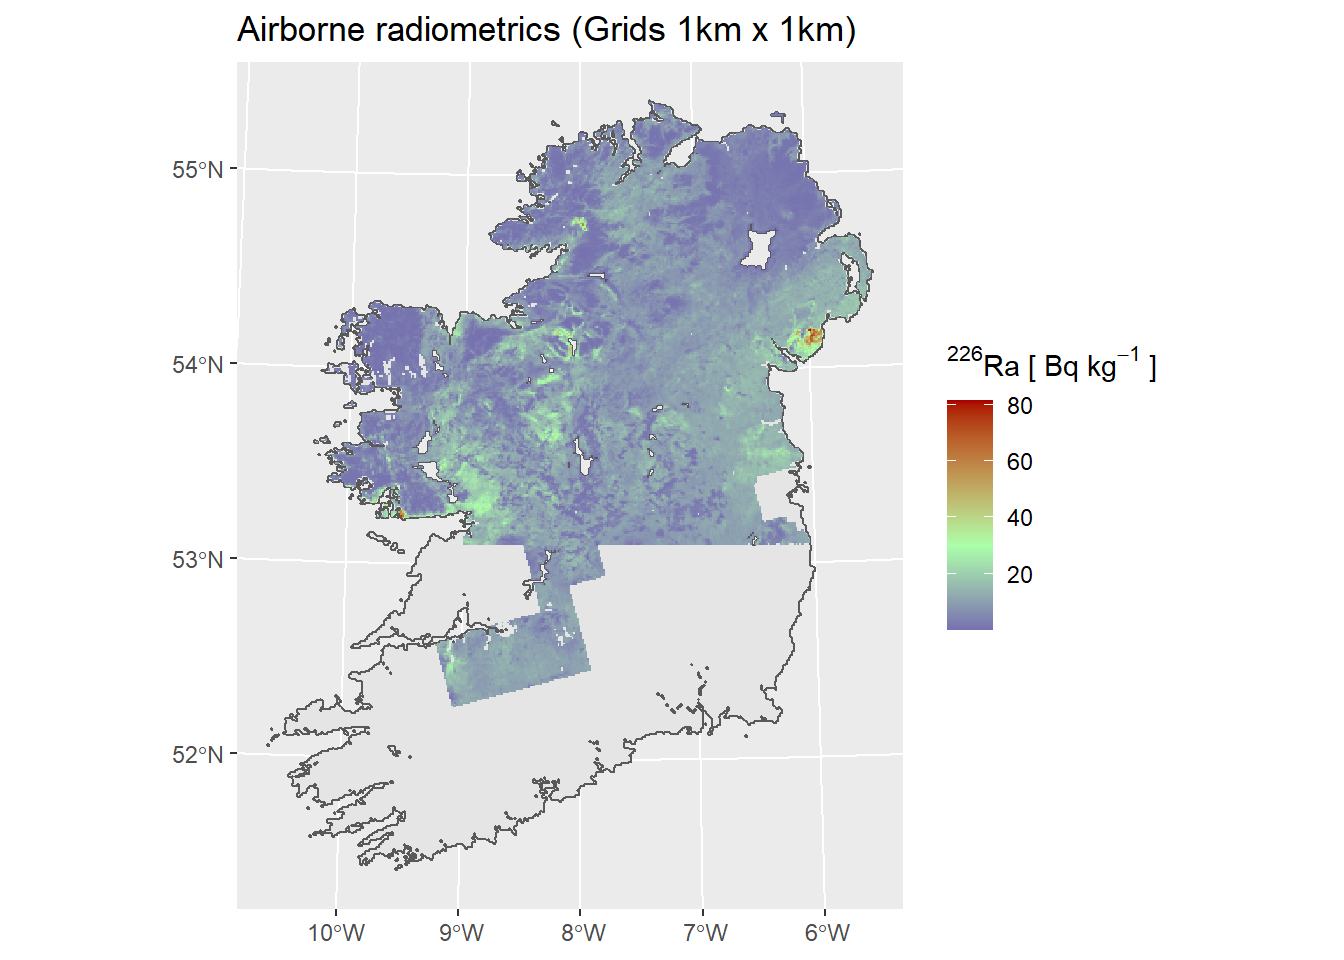
\includegraphics{Article_Code_files/figure-latex/Plot_eRa-1} \end{center}

\hypertarget{all-ireland-quaternary-map-scale-1500.000}{%
\subsection{All-Ireland Quaternary map (scale
1:500.000)}\label{all-ireland-quaternary-map-scale-1500.000}}

\begin{Shaded}
\begin{Highlighting}[]
\NormalTok{  QG \textless{}{-}}\StringTok{ }\KeywordTok{read\_sf}\NormalTok{(}\StringTok{"Rdata/GSI\_Quaternary\_500k/QG\_500k.shp"}\NormalTok{) }\OperatorTok{\%\textgreater{}\%}\StringTok{ }
\StringTok{    }\KeywordTok{mutate}\NormalTok{(}\DataTypeTok{Sediment\_5 =} \KeywordTok{as\_factor}\NormalTok{(Sediment\_}\DecValTok{5}\NormalTok{)) }\OperatorTok{\%\textgreater{}\%}
\StringTok{    }\KeywordTok{group\_by}\NormalTok{(Sediment\_}\DecValTok{5}\NormalTok{) }\OperatorTok{\%\textgreater{}\%}
\StringTok{    }\KeywordTok{summarise}\NormalTok{(}\DataTypeTok{N =} \KeywordTok{n}\NormalTok{(),}
              \DataTypeTok{area\_sq\_km =} \KeywordTok{sum}\NormalTok{(area\_sq\_km),}
              \DataTypeTok{label =} \KeywordTok{first}\NormalTok{(label)) }\OperatorTok{\%\textgreater{}\%}
\StringTok{    }\KeywordTok{ungroup}\NormalTok{()}
\end{Highlighting}
\end{Shaded}

\hypertarget{aquifer-type}{%
\subsection{Aquifer Type}\label{aquifer-type}}

\begin{Shaded}
\begin{Highlighting}[]
\NormalTok{AQ \textless{}{-}}\StringTok{ }\KeywordTok{read\_sf}\NormalTok{(}\StringTok{"Rdata/Groundwater/IRL\_AQUIFER\_BEDROCK\_ITM.shp"}\NormalTok{) }\OperatorTok{\%\textgreater{}\%}
\StringTok{    }\NormalTok{rmapshaper}\OperatorTok{::}\KeywordTok{ms\_simplify}\NormalTok{(}\DataTypeTok{keep =} \FloatTok{0.01}\NormalTok{, }\DataTypeTok{keep\_shapes =} \OtherTok{TRUE}\NormalTok{) }\OperatorTok{\%\textgreater{}\%}
\StringTok{    }\KeywordTok{st\_make\_valid}\NormalTok{()}
  
\NormalTok{  Karst \textless{}{-}}\StringTok{ }\NormalTok{AQ }\OperatorTok{\%\textgreater{}\%}\StringTok{ }
\StringTok{    }\KeywordTok{group\_by}\NormalTok{(AQUIFERCAT) }\OperatorTok{\%\textgreater{}\%}
\StringTok{    }\KeywordTok{summarize}\NormalTok{(}\DataTypeTok{AQUIFER\_DE =} \KeywordTok{first}\NormalTok{(AQUIFER\_DE)) }\OperatorTok{\%\textgreater{}\%}
\StringTok{    }\KeywordTok{ungroup}\NormalTok{() }\OperatorTok{\%\textgreater{}\%}
\StringTok{    }\KeywordTok{filter}\NormalTok{(AQUIFERCAT }\OperatorTok{!=}\StringTok{ "Lake"} \OperatorTok{\&}\StringTok{ }\NormalTok{AQUIFERCAT }\OperatorTok{!=}\StringTok{ "Unclas"}\NormalTok{) }\OperatorTok{\%\textgreater{}\%}
\StringTok{    }\KeywordTok{mutate}\NormalTok{(}\DataTypeTok{Karst =} \KeywordTok{case\_when}\NormalTok{(}
\NormalTok{      AQUIFERCAT }\OperatorTok{==}\StringTok{ "Lk"}     \OperatorTok{\textasciitilde{}}\StringTok{ "TRUE"}\NormalTok{,}
\NormalTok{      AQUIFERCAT }\OperatorTok{==}\StringTok{ "LkNI"}   \OperatorTok{\textasciitilde{}}\StringTok{ "TRUE"}\NormalTok{,}
\NormalTok{      AQUIFERCAT }\OperatorTok{==}\StringTok{ "Ll"}     \OperatorTok{\textasciitilde{}}\StringTok{ "FALSE"}\NormalTok{,                         }
\NormalTok{      AQUIFERCAT }\OperatorTok{==}\StringTok{ "LlNI"}   \OperatorTok{\textasciitilde{}}\StringTok{ "FALSE"}\NormalTok{,                 }
\NormalTok{      AQUIFERCAT }\OperatorTok{==}\StringTok{ "Lm"}     \OperatorTok{\textasciitilde{}}\StringTok{ "FALSE"}\NormalTok{,                }
\NormalTok{      AQUIFERCAT }\OperatorTok{==}\StringTok{ "LmNI"}   \OperatorTok{\textasciitilde{}}\StringTok{ "FALSE"}\NormalTok{,              }
\NormalTok{      AQUIFERCAT }\OperatorTok{==}\StringTok{ "NI\_Un*"} \OperatorTok{\textasciitilde{}}\StringTok{ "FALSE"}\NormalTok{,                  }
\NormalTok{      AQUIFERCAT }\OperatorTok{==}\StringTok{ "PINIl"}  \OperatorTok{\textasciitilde{}}\StringTok{ "FALSE"}\NormalTok{,       }
\NormalTok{      AQUIFERCAT }\OperatorTok{==}\StringTok{ "Pl"}     \OperatorTok{\textasciitilde{}}\StringTok{ "FALSE"}\NormalTok{,      }
\NormalTok{      AQUIFERCAT }\OperatorTok{==}\StringTok{ "PlNI"}   \OperatorTok{\textasciitilde{}}\StringTok{ "FALSE"}\NormalTok{,     }
\NormalTok{      AQUIFERCAT }\OperatorTok{==}\StringTok{ "Pu"}     \OperatorTok{\textasciitilde{}}\StringTok{ "FALSE"}\NormalTok{,    }
\NormalTok{      AQUIFERCAT }\OperatorTok{==}\StringTok{ "PuNI"}   \OperatorTok{\textasciitilde{}}\StringTok{ "FALSE"}\NormalTok{,   }
\NormalTok{      AQUIFERCAT }\OperatorTok{==}\StringTok{ "Rf"}     \OperatorTok{\textasciitilde{}}\StringTok{ "FALSE"}\NormalTok{,  }
\NormalTok{      AQUIFERCAT }\OperatorTok{==}\StringTok{ "Rf/Rk"}  \OperatorTok{\textasciitilde{}}\StringTok{ "TRUE"}\NormalTok{ , }
\NormalTok{      AQUIFERCAT }\OperatorTok{==}\StringTok{ "RfNI"}   \OperatorTok{\textasciitilde{}}\StringTok{ "FALSE"}\NormalTok{,}
\NormalTok{      AQUIFERCAT }\OperatorTok{==}\StringTok{ "Rk"}     \OperatorTok{\textasciitilde{}}\StringTok{ "TRUE"}\NormalTok{,}
\NormalTok{      AQUIFERCAT }\OperatorTok{==}\StringTok{ "Rkc"}    \OperatorTok{\textasciitilde{}}\StringTok{ "TRUE"}\NormalTok{,}
\NormalTok{      AQUIFERCAT }\OperatorTok{==}\StringTok{ "RkcNI"}  \OperatorTok{\textasciitilde{}}\StringTok{ "TRUE"}\NormalTok{,}
\NormalTok{      AQUIFERCAT }\OperatorTok{==}\StringTok{ "Rkd"}    \OperatorTok{\textasciitilde{}}\StringTok{ "TRUE"}\NormalTok{,}
\NormalTok{      AQUIFERCAT }\OperatorTok{==}\StringTok{ "RkNI"}   \OperatorTok{\textasciitilde{}}\StringTok{ "TRUE"}\NormalTok{,}
      \OtherTok{TRUE} \OperatorTok{\textasciitilde{}}\StringTok{ }\KeywordTok{as.character}\NormalTok{(AQUIFERCAT))}
\NormalTok{    ) }\OperatorTok{\%\textgreater{}\%}
\StringTok{    }\KeywordTok{group\_by}\NormalTok{(Karst) }\OperatorTok{\%\textgreater{}\%}
\StringTok{    }\KeywordTok{summarise}\NormalTok{(}\DataTypeTok{N =} \KeywordTok{n}\NormalTok{()) }\OperatorTok{\%\textgreater{}\%}
\StringTok{    }\KeywordTok{ungroup}\NormalTok{()}
\end{Highlighting}
\end{Shaded}

\hypertarget{subsoil-permeability}{%
\subsection{Subsoil permeability}\label{subsoil-permeability}}

Load \emph{SP\_GW\_naQG.shp} file; output of the R-script:
\emph{SP\_Groundwater\_recharge.R}.

\begin{Shaded}
\begin{Highlighting}[]
\NormalTok{  SP \textless{}{-}}\StringTok{ }\KeywordTok{read\_sf}\NormalTok{(}\StringTok{"Rresults/Soil\_Permeability/SP\_GW\_naQG.shp"}\NormalTok{) }\OperatorTok{\%\textgreater{}\%}
\StringTok{    }\KeywordTok{rename}\NormalTok{(}\DataTypeTok{Perm =}\NormalTok{ PERM) }\OperatorTok{\%\textgreater{}\%}
\StringTok{    }\KeywordTok{mutate}\NormalTok{(}\DataTypeTok{Perm =} \KeywordTok{factor}\NormalTok{(Perm,}
                         \DataTypeTok{levels =} \KeywordTok{c}\NormalTok{(}\StringTok{"H"}\NormalTok{, }\StringTok{"M"}\NormalTok{, }\StringTok{"L"}\NormalTok{),}
                         \DataTypeTok{ordered =} \OtherTok{TRUE}\NormalTok{)) }
\end{Highlighting}
\end{Shaded}

Rasterize: convert Subsoil Permeability shapefile (SP) to a raster file
with a resolution of 1km x 1 km).

\begin{enumerate}
\def\labelenumi{\alph{enumi})}
\tightlist
\item
  Make grids equal to the cell grids of eU data (1km x 1km)
\end{enumerate}

\begin{Shaded}
\begin{Highlighting}[]
\NormalTok{  grd\_res\_x \textless{}{-}}\StringTok{ }\DecValTok{1000} \CommentTok{\# m}
\NormalTok{  grd\_res\_y \textless{}{-}}\StringTok{ }\DecValTok{1000} \CommentTok{\# m}
\NormalTok{  grd \textless{}{-}}\StringTok{ }\KeywordTok{st\_as\_stars}\NormalTok{(}\KeywordTok{st\_bbox}\NormalTok{(eU\_Grids1km),}
     \DataTypeTok{nx =}\NormalTok{ (}\KeywordTok{st\_bbox}\NormalTok{(eU\_Grids1km)[}\DecValTok{3}\NormalTok{] }\OperatorTok{{-}}\StringTok{ }\KeywordTok{st\_bbox}\NormalTok{(eU\_Grids1km)[}\DecValTok{1}\NormalTok{]) }\OperatorTok{/}\StringTok{ }\NormalTok{grd\_res\_x,}
     \DataTypeTok{ny =}\NormalTok{ (}\KeywordTok{st\_bbox}\NormalTok{(eU\_Grids1km)[}\DecValTok{4}\NormalTok{] }\OperatorTok{{-}}\StringTok{ }\KeywordTok{st\_bbox}\NormalTok{(eU\_Grids1km)[}\DecValTok{2}\NormalTok{]) }\OperatorTok{/}\StringTok{ }\NormalTok{grd\_res\_y,}
     \DataTypeTok{xlim =} \KeywordTok{c}\NormalTok{(}\KeywordTok{st\_bbox}\NormalTok{(eU\_Grids1km)[}\DecValTok{1}\NormalTok{], }\KeywordTok{st\_bbox}\NormalTok{(eU\_Grids1km)[}\DecValTok{3}\NormalTok{]),}
     \DataTypeTok{ylim =} \KeywordTok{c}\NormalTok{(}\KeywordTok{st\_bbox}\NormalTok{(eU\_Grids1km)[}\DecValTok{2}\NormalTok{], }\KeywordTok{st\_bbox}\NormalTok{(eU\_Grids1km)[}\DecValTok{4}\NormalTok{]),}
     \DataTypeTok{values =} \OtherTok{NA\_real\_}\NormalTok{)}
\end{Highlighting}
\end{Shaded}

\begin{enumerate}
\def\labelenumi{\alph{enumi})}
\setcounter{enumi}{1}
\tightlist
\item
  Rasterize
\end{enumerate}

\begin{Shaded}
\begin{Highlighting}[]
\NormalTok{  SP\_Raster \textless{}{-}}\StringTok{ }\NormalTok{stars}\OperatorTok{::}\KeywordTok{st\_rasterize}\NormalTok{(SP[}\StringTok{"Perm"}\NormalTok{], grd) }\OperatorTok{\%\textgreater{}\%}
\StringTok{    }\KeywordTok{mutate}\NormalTok{(}\DataTypeTok{Perm\_class =} \KeywordTok{case\_when}\NormalTok{(}
\NormalTok{      ID }\OperatorTok{==}\StringTok{ }\DecValTok{1}   \OperatorTok{\textasciitilde{}}\StringTok{ "H"}\NormalTok{,}
\NormalTok{      ID }\OperatorTok{==}\StringTok{ }\DecValTok{2}   \OperatorTok{\textasciitilde{}}\StringTok{ "H"}\NormalTok{,}
\NormalTok{      ID }\OperatorTok{==}\StringTok{ }\DecValTok{3}   \OperatorTok{\textasciitilde{}}\StringTok{ "H"}\NormalTok{,}
\NormalTok{      ID }\OperatorTok{==}\StringTok{ }\DecValTok{4}   \OperatorTok{\textasciitilde{}}\StringTok{ "H"}\NormalTok{,}
\NormalTok{      ID }\OperatorTok{==}\StringTok{ }\DecValTok{5}   \OperatorTok{\textasciitilde{}}\StringTok{ "H"}\NormalTok{,}
\NormalTok{      ID }\OperatorTok{==}\StringTok{ }\DecValTok{6}   \OperatorTok{\textasciitilde{}}\StringTok{ "M"}\NormalTok{,}
\NormalTok{      ID }\OperatorTok{==}\StringTok{ }\DecValTok{7}   \OperatorTok{\textasciitilde{}}\StringTok{ "M"}\NormalTok{,}
\NormalTok{      ID }\OperatorTok{==}\StringTok{ }\DecValTok{8}   \OperatorTok{\textasciitilde{}}\StringTok{ "M"}\NormalTok{,}
\NormalTok{      ID }\OperatorTok{==}\StringTok{ }\DecValTok{9}   \OperatorTok{\textasciitilde{}}\StringTok{ "M"}\NormalTok{,}
\NormalTok{      ID }\OperatorTok{==}\StringTok{ }\DecValTok{10}  \OperatorTok{\textasciitilde{}}\StringTok{ "M"}\NormalTok{,}
\NormalTok{      ID }\OperatorTok{==}\StringTok{ }\DecValTok{11}  \OperatorTok{\textasciitilde{}}\StringTok{ "M"}\NormalTok{,}
\NormalTok{      ID }\OperatorTok{==}\StringTok{ }\DecValTok{12}  \OperatorTok{\textasciitilde{}}\StringTok{ "L"}\NormalTok{,}
\NormalTok{      ID }\OperatorTok{==}\StringTok{ }\DecValTok{13}  \OperatorTok{\textasciitilde{}}\StringTok{ "L"}\NormalTok{,}
\NormalTok{      ID }\OperatorTok{==}\StringTok{ }\DecValTok{14}  \OperatorTok{\textasciitilde{}}\StringTok{ "L"}\NormalTok{,}
\NormalTok{      ID }\OperatorTok{==}\StringTok{ }\DecValTok{15}  \OperatorTok{\textasciitilde{}}\StringTok{ "L"}\NormalTok{,}
      \KeywordTok{is.na}\NormalTok{(ID) }\OperatorTok{\textasciitilde{}}\StringTok{ "NA"}\NormalTok{ )) }\OperatorTok{\%\textgreater{}\%}
\StringTok{    }\KeywordTok{mutate}\NormalTok{(}\DataTypeTok{Perm\_class =} \KeywordTok{factor}\NormalTok{(Perm\_class, }
                               \DataTypeTok{levels =} \KeywordTok{c}\NormalTok{(}\StringTok{"H"}\NormalTok{, }\StringTok{"M"}\NormalTok{, }\StringTok{"L"}\NormalTok{, }\StringTok{"NA"}\NormalTok{),}
                               \DataTypeTok{ordered =} \OtherTok{TRUE}\NormalTok{)) }\OperatorTok{\%\textgreater{}\%}
\StringTok{    }\KeywordTok{st\_crop}\NormalTok{(eU\_Grids1km)}
\end{Highlighting}
\end{Shaded}

\hypertarget{results}{%
\section{Results}\label{results}}

\hypertarget{soil-gas-radon-predictions-based-on-airborne-radiometrics-eu}{%
\subsection{Soil-gas radon predictions based on airborne radiometrics
(eU)}\label{soil-gas-radon-predictions-based-on-airborne-radiometrics-eu}}

\begin{enumerate}
\def\labelenumi{\alph{enumi})}
\tightlist
\item
  Soil Parameters:
\end{enumerate}

\begin{itemize}
\tightlist
\item
  e \textasciitilde{} N(0.29, 0.03); Yu et al 1993: Range approx. from
  0.13 to 0.37
\item
  d \textasciitilde{} N(1.35, 0.06); Yu et al 1993: Range dry density
  1.1 - 1.6; Creamer et al 2016 (Irish soils) bulk density mainly
  1.1-1.3 and \textgreater1.4 g m-3
\item
  n \textasciitilde{} N(0.30, 0.07); Yu et al 1993: Effective Porosity
  range approx. from 0.02 to 0.53
\item
  Water influence (SF) \textasciitilde{} uniform distribution on the
  interval from min (0.4) to max (0.6)
\end{itemize}

\begin{Shaded}
\begin{Highlighting}[]
  \KeywordTok{set.seed}\NormalTok{(}\DecValTok{1}\NormalTok{) }\CommentTok{\# Make the analysis reproducible}
  
\NormalTok{  e  \textless{}{-}}\StringTok{ }\KeywordTok{rnorm}\NormalTok{(}\DecValTok{1000}\NormalTok{, }\DataTypeTok{mean =} \FloatTok{0.29}\NormalTok{, }\DataTypeTok{sd =} \FloatTok{0.03}\NormalTok{)}
\NormalTok{  d  \textless{}{-}}\StringTok{ }\KeywordTok{rnorm}\NormalTok{(}\DecValTok{1000}\NormalTok{, }\DataTypeTok{mean =} \FloatTok{1.35}\NormalTok{, }\DataTypeTok{sd =} \FloatTok{0.06}\NormalTok{)}
\NormalTok{  n  \textless{}{-}}\StringTok{ }\KeywordTok{rnorm}\NormalTok{(}\DecValTok{1000}\NormalTok{, }\DataTypeTok{mean =} \FloatTok{0.30}\NormalTok{, }\DataTypeTok{sd =} \FloatTok{0.07}\NormalTok{)}
\NormalTok{  SF \textless{}{-}}\StringTok{ }\KeywordTok{runif}\NormalTok{(}\DecValTok{1000}\NormalTok{, }\DataTypeTok{min =} \FloatTok{0.4}\NormalTok{, }\DataTypeTok{max =} \FloatTok{0.6}\NormalTok{)}
\NormalTok{  id \textless{}{-}}\StringTok{ "g90164"} 
\NormalTok{  Ra \textless{}{-}}\StringTok{ }\KeywordTok{rnorm}\NormalTok{(}\DecValTok{1000}\NormalTok{,}
              \DataTypeTok{mean =}\NormalTok{ eU\_Grids1km[eU\_Grids1km}\OperatorTok{$}\NormalTok{SP\_ID }\OperatorTok{==}\StringTok{ }\NormalTok{id, ]}\OperatorTok{$}\NormalTok{AM\_Ra226,}
              \DataTypeTok{sd   =}\NormalTok{ eU\_Grids1km[eU\_Grids1km}\OperatorTok{$}\NormalTok{SP\_ID }\OperatorTok{==}\StringTok{ }\NormalTok{id, ]}\OperatorTok{$}\NormalTok{SD\_Ra226}
\NormalTok{              )}
  
  \KeywordTok{par}\NormalTok{(}\DataTypeTok{mfrow =} \KeywordTok{c}\NormalTok{(}\DecValTok{2}\NormalTok{,}\DecValTok{3}\NormalTok{))}
  \KeywordTok{hist}\NormalTok{(e, }\DataTypeTok{col =} \DecValTok{2}\NormalTok{, }\DataTypeTok{breaks =} \DecValTok{15}\NormalTok{, }\DataTypeTok{main =} \StringTok{"Emanation coefficient"}\NormalTok{)}
  \KeywordTok{hist}\NormalTok{(d, }\DataTypeTok{col =} \DecValTok{2}\NormalTok{, }\DataTypeTok{breaks =} \DecValTok{15}\NormalTok{, }\DataTypeTok{main =} \StringTok{"Soil density"}\NormalTok{,}
       \DataTypeTok{xlab =} \KeywordTok{expression}\NormalTok{(d }\OperatorTok{*}\StringTok{ " ["} \OperatorTok{*}\NormalTok{g }\OperatorTok{*}\StringTok{" "}\OperatorTok{*}\StringTok{ }\NormalTok{cm}\OperatorTok{\^{}{-}}\DecValTok{3} \OperatorTok{*}\StringTok{ "]"}\NormalTok{))}
  \KeywordTok{hist}\NormalTok{(n, }\DataTypeTok{col =} \DecValTok{2}\NormalTok{, }\DataTypeTok{breaks =} \DecValTok{15}\NormalTok{, }\DataTypeTok{main =} \StringTok{"Effective porosity"}\NormalTok{)}
  \KeywordTok{hist}\NormalTok{(SF, }\DataTypeTok{col =} \DecValTok{2}\NormalTok{, }\DataTypeTok{breaks =} \DecValTok{15}\NormalTok{, }\DataTypeTok{main =} \StringTok{"Water saturation"}\NormalTok{)}
  \KeywordTok{hist}\NormalTok{(Ra, }\DataTypeTok{col =} \DecValTok{2}\NormalTok{, }\DataTypeTok{breaks =} \DecValTok{15}\NormalTok{, }\DataTypeTok{main =} \StringTok{"Ra{-}226"}\NormalTok{)}
\end{Highlighting}
\end{Shaded}

\begin{center}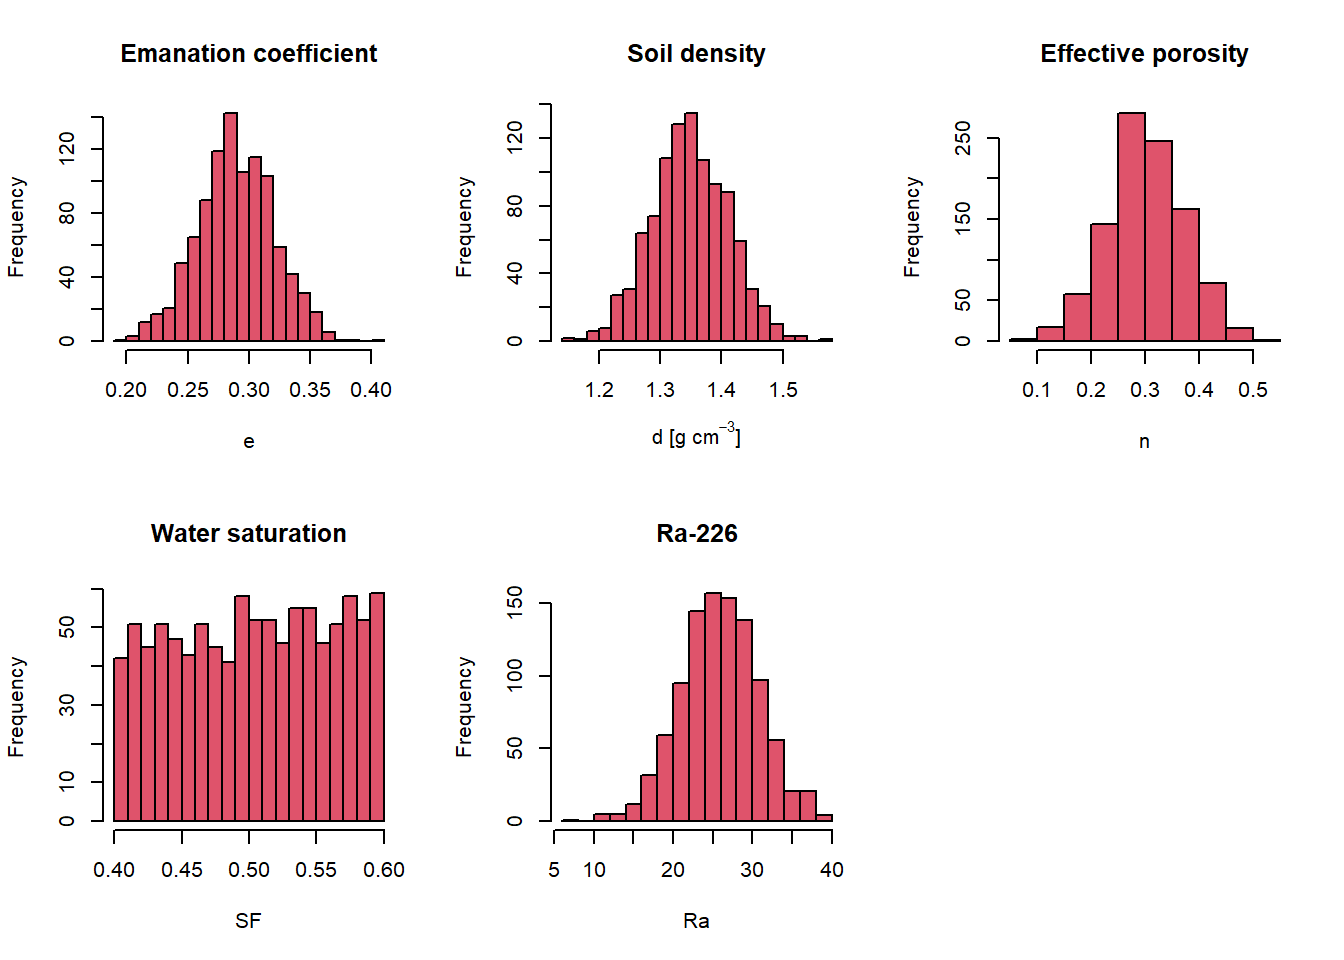
\includegraphics{Article_Code_files/figure-latex/Parameters-1} \end{center}

\begin{enumerate}
\def\labelenumi{\alph{enumi})}
\setcounter{enumi}{1}
\tightlist
\item
  Simulations
\end{enumerate}

Radon concentration in soil-gas:

\[C_{Rn} [kBq m^{-3}] = \frac{C_{Ra} [Bq kg^{-1}] \times e \times \rho [g m^{-3}]}{n} \times \frac{1}{1 - S_F + S_FK_{W/Air}}\]

\begin{Shaded}
\begin{Highlighting}[]
  \KeywordTok{set.seed}\NormalTok{(}\DecValTok{1}\NormalTok{) }\CommentTok{\# Make the analysis reproducible}

\NormalTok{  rep \textless{}{-}}\StringTok{ }\DecValTok{1000}
\NormalTok{  SG\_MCS \textless{}{-}}\StringTok{ }\KeywordTok{matrix}\NormalTok{(}\OtherTok{NA}\NormalTok{, }\DataTypeTok{nrow =} \KeywordTok{dim}\NormalTok{(eU\_Grids1km)[}\DecValTok{1}\NormalTok{], }\DataTypeTok{ncol =}\NormalTok{ rep}\OperatorTok{+}\DecValTok{1}\NormalTok{)}
  \ControlFlowTok{for}\NormalTok{ (i }\ControlFlowTok{in} \DecValTok{1}\OperatorTok{:}\NormalTok{rep) \{}
\NormalTok{    Ra \textless{}{-}}\StringTok{ }\KeywordTok{rnorm}\NormalTok{(}\KeywordTok{dim}\NormalTok{(eU\_Grids1km)[}\DecValTok{1}\NormalTok{],}
\NormalTok{                eU\_Grids1km}\OperatorTok{$}\NormalTok{AM\_Ra226,}
\NormalTok{                eU\_Grids1km}\OperatorTok{$}\NormalTok{SD\_Ra226)}
\NormalTok{    e  \textless{}{-}}\StringTok{ }\KeywordTok{rnorm}\NormalTok{(}\KeywordTok{dim}\NormalTok{(eU\_Grids1km)[}\DecValTok{1}\NormalTok{], }\FloatTok{0.29}\NormalTok{, }\FloatTok{0.03}\NormalTok{)}
\NormalTok{    d  \textless{}{-}}\StringTok{ }\KeywordTok{rnorm}\NormalTok{(}\KeywordTok{dim}\NormalTok{(eU\_Grids1km)[}\DecValTok{1}\NormalTok{], }\FloatTok{1.35}\NormalTok{, }\FloatTok{0.06}\NormalTok{)}
\NormalTok{    n  \textless{}{-}}\StringTok{ }\KeywordTok{rnorm}\NormalTok{(}\KeywordTok{dim}\NormalTok{(eU\_Grids1km)[}\DecValTok{1}\NormalTok{], }\FloatTok{0.30}\NormalTok{, }\FloatTok{0.07}\NormalTok{)}
\NormalTok{    SF \textless{}{-}}\StringTok{ }\KeywordTok{runif}\NormalTok{(}\KeywordTok{dim}\NormalTok{(eU\_Grids1km)[}\DecValTok{1}\NormalTok{], }\FloatTok{0.40}\NormalTok{, }\FloatTok{0.60}\NormalTok{)}
\NormalTok{    SG\_MCS[ ,i}\OperatorTok{+}\DecValTok{1}\NormalTok{] \textless{}{-}}\StringTok{ }\NormalTok{(Ra}\OperatorTok{*}\NormalTok{e}\OperatorTok{*}\NormalTok{d}\OperatorTok{/}\NormalTok{n)}\OperatorTok{*}\NormalTok{(}\DecValTok{1}\OperatorTok{/}\NormalTok{(}\DecValTok{1}\OperatorTok{{-}}\NormalTok{SF}\OperatorTok{+}\NormalTok{(}\FloatTok{0.25}\OperatorTok{*}\NormalTok{SF)))}
\NormalTok{  \}}
\NormalTok{  SG\_MCS \textless{}{-}}\StringTok{ }\KeywordTok{as.data.frame}\NormalTok{(SG\_MCS)}
  \KeywordTok{names}\NormalTok{(SG\_MCS) \textless{}{-}}\StringTok{ }\KeywordTok{c}\NormalTok{(}\StringTok{"SP\_ID"}\NormalTok{, }\KeywordTok{c}\NormalTok{(}\DecValTok{1}\OperatorTok{:}\NormalTok{rep))}
\NormalTok{  SG\_MCS}\OperatorTok{$}\NormalTok{SP\_ID \textless{}{-}}\StringTok{ }\NormalTok{eU\_Grids1km}\OperatorTok{$}\NormalTok{SP\_ID}
   
\NormalTok{  SG\_MCS \textless{}{-}}\StringTok{ }\KeywordTok{as\_tibble}\NormalTok{(SG\_MCS)}
\NormalTok{  SG\_MCS}
\end{Highlighting}
\end{Shaded}

\begin{enumerate}
\def\labelenumi{\alph{enumi})}
\setcounter{enumi}{2}
\tightlist
\item
  Percentiles:
\end{enumerate}

\begin{Shaded}
\begin{Highlighting}[]
\NormalTok{  SG\_MCS\_T \textless{}{-}}\StringTok{ }\KeywordTok{t}\NormalTok{(SG\_MCS[,}\DecValTok{2}\OperatorTok{:}\NormalTok{rep])}
  
\NormalTok{  SG\_MCS\_P95 \textless{}{-}}\StringTok{ }\KeywordTok{matrix}\NormalTok{(}\OtherTok{NA}\NormalTok{, }\DataTypeTok{nrow =} \KeywordTok{dim}\NormalTok{(eU\_Grids1km)[}\DecValTok{1}\NormalTok{], }\DataTypeTok{ncol =} \DecValTok{8}\NormalTok{)  }
  \ControlFlowTok{for}\NormalTok{ (i }\ControlFlowTok{in} \DecValTok{1}\OperatorTok{:}\KeywordTok{dim}\NormalTok{(eU\_Grids1km)[}\DecValTok{1}\NormalTok{]) \{}
\NormalTok{    SG\_MCS\_P95[i,}\DecValTok{2}\NormalTok{] \textless{}{-}}\StringTok{ }\KeywordTok{quantile}\NormalTok{(SG\_MCS\_T[,i], }\FloatTok{0.025}\NormalTok{)}
\NormalTok{    SG\_MCS\_P95[i,}\DecValTok{3}\NormalTok{] \textless{}{-}}\StringTok{ }\KeywordTok{quantile}\NormalTok{(SG\_MCS\_T[,i], }\FloatTok{0.05}\NormalTok{)}
\NormalTok{    SG\_MCS\_P95[i,}\DecValTok{4}\NormalTok{] \textless{}{-}}\StringTok{ }\KeywordTok{quantile}\NormalTok{(SG\_MCS\_T[,i], }\FloatTok{0.25}\NormalTok{)}
\NormalTok{    SG\_MCS\_P95[i,}\DecValTok{5}\NormalTok{] \textless{}{-}}\StringTok{ }\KeywordTok{quantile}\NormalTok{(SG\_MCS\_T[,i], }\FloatTok{0.50}\NormalTok{)}
\NormalTok{    SG\_MCS\_P95[i,}\DecValTok{6}\NormalTok{] \textless{}{-}}\StringTok{ }\KeywordTok{quantile}\NormalTok{(SG\_MCS\_T[,i], }\FloatTok{0.75}\NormalTok{)}
\NormalTok{    SG\_MCS\_P95[i,}\DecValTok{7}\NormalTok{] \textless{}{-}}\StringTok{ }\KeywordTok{quantile}\NormalTok{(SG\_MCS\_T[,i], }\FloatTok{0.95}\NormalTok{)}
\NormalTok{    SG\_MCS\_P95[i,}\DecValTok{8}\NormalTok{] \textless{}{-}}\StringTok{ }\KeywordTok{quantile}\NormalTok{(SG\_MCS\_T[,i], }\FloatTok{0.975}\NormalTok{)}
\NormalTok{  \}}
  
\NormalTok{  SG\_MCS\_P95 \textless{}{-}}\StringTok{ }\KeywordTok{as.data.frame}\NormalTok{(SG\_MCS\_P95)}
  \KeywordTok{names}\NormalTok{(SG\_MCS\_P95) \textless{}{-}}\StringTok{ }\KeywordTok{c}\NormalTok{(}\StringTok{"SP\_ID"}\NormalTok{,}\StringTok{"Rn\_P025"}\NormalTok{,}\StringTok{"Rn\_P05"}\NormalTok{,}\StringTok{"Rn\_P25"}\NormalTok{,}
                         \StringTok{"Rn\_P50"}\NormalTok{,}\StringTok{"Rn\_P75"}\NormalTok{,}\StringTok{"Rn\_P95"}\NormalTok{,}\StringTok{"Rn\_P975"}\NormalTok{)}
\NormalTok{  SG\_MCS\_P95}\OperatorTok{$}\NormalTok{SP\_ID \textless{}{-}}\StringTok{ }\NormalTok{SG\_MCS}\OperatorTok{$}\NormalTok{SP\_ID}
\NormalTok{  SG\_MCS\_P95 \textless{}{-}}\StringTok{ }\KeywordTok{as\_tibble}\NormalTok{(SG\_MCS\_P95)}
  
\NormalTok{  eU\_Grids1km \textless{}{-}}\StringTok{ }\KeywordTok{left\_join}\NormalTok{(eU\_Grids1km, SG\_MCS\_P95, }\DataTypeTok{by =} \StringTok{"SP\_ID"}\NormalTok{)}
\NormalTok{  eU\_Grids1km}
\end{Highlighting}
\end{Shaded}

\begin{enumerate}
\def\labelenumi{\alph{enumi})}
\setcounter{enumi}{3}
\tightlist
\item
  Soil gas radon classification based on eU (Rn predictions - percentile
  75\%):
\end{enumerate}

\begin{itemize}
\tightlist
\item
  Extremely High: \textgreater= 100
\item
  Very High: 70 - 100
\item
  High: 50 - 70
\item
  Moderate: 30 - 50
\item
  Low: 10 - 30
\item
  Very Low: \textless{} 10
\end{itemize}

\begin{Shaded}
\begin{Highlighting}[]
\NormalTok{  eU\_Grids1km \textless{}{-}}\StringTok{ }\NormalTok{eU\_Grids1km }\OperatorTok{\%\textgreater{}\%}
\StringTok{    }\KeywordTok{mutate}\NormalTok{(}\DataTypeTok{Rn\_class =} \KeywordTok{case\_when}\NormalTok{(}
\NormalTok{      Rn\_P75 }\OperatorTok{\textgreater{}=}\StringTok{ }\DecValTok{100}              \OperatorTok{\textasciitilde{}}\StringTok{ "EH"}\NormalTok{,}
\NormalTok{      Rn\_P75 }\OperatorTok{\textgreater{}=}\StringTok{ }\DecValTok{70} \OperatorTok{\&}\StringTok{ }\NormalTok{Rn\_P75 }\OperatorTok{\textless{}}\StringTok{ }\DecValTok{100} \OperatorTok{\textasciitilde{}}\StringTok{ "VH"}\NormalTok{,}
\NormalTok{      Rn\_P75 }\OperatorTok{\textgreater{}=}\StringTok{ }\DecValTok{50} \OperatorTok{\&}\StringTok{ }\NormalTok{Rn\_P75 }\OperatorTok{\textless{}}\StringTok{  }\DecValTok{70} \OperatorTok{\textasciitilde{}}\StringTok{  "H"}\NormalTok{,}
\NormalTok{      Rn\_P75 }\OperatorTok{\textgreater{}=}\StringTok{ }\DecValTok{30} \OperatorTok{\&}\StringTok{ }\NormalTok{Rn\_P75 }\OperatorTok{\textless{}}\StringTok{  }\DecValTok{50} \OperatorTok{\textasciitilde{}}\StringTok{  "M"}\NormalTok{,                 }
\NormalTok{      Rn\_P75 }\OperatorTok{\textgreater{}=}\StringTok{ }\DecValTok{10} \OperatorTok{\&}\StringTok{ }\NormalTok{Rn\_P75 }\OperatorTok{\textless{}}\StringTok{  }\DecValTok{30} \OperatorTok{\textasciitilde{}}\StringTok{  "L"}\NormalTok{,                }
\NormalTok{      Rn\_P75 }\OperatorTok{\textless{}}\StringTok{  }\DecValTok{10}                \OperatorTok{\textasciitilde{}}\StringTok{ "VL"}\NormalTok{,}
      \OtherTok{TRUE} \OperatorTok{\textasciitilde{}}\StringTok{ }\KeywordTok{as.character}\NormalTok{(Rn\_P75)}
\NormalTok{    )}
\NormalTok{    ) }\OperatorTok{\%\textgreater{}\%}
\StringTok{    }\KeywordTok{mutate}\NormalTok{(}\DataTypeTok{Rn\_class =} \KeywordTok{factor}\NormalTok{(Rn\_class, }
                             \DataTypeTok{levels =} \KeywordTok{c}\NormalTok{(}\StringTok{"EH"}\NormalTok{, }\StringTok{"VH"}\NormalTok{, }\StringTok{"H"}\NormalTok{, }\StringTok{"M"}\NormalTok{, }\StringTok{"L"}\NormalTok{, }\StringTok{"VL"}\NormalTok{),}
                             \DataTypeTok{ordered =} \OtherTok{TRUE}
\NormalTok{    )}
\NormalTok{    )}
\end{Highlighting}
\end{Shaded}

\hypertarget{radon-potential-map}{%
\subsection{Radon Potential map}\label{radon-potential-map}}

\begin{enumerate}
\def\labelenumi{\alph{enumi})}
\tightlist
\item
  Merge Rn\_class and SP in one dataset (by grids of 1km x 1km):
\end{enumerate}

\begin{itemize}
\tightlist
\item
  Create a dataframe with \emph{Rn} values (Rn\_class)
\item
  Transform SP\_Raster to points (\emph{Perm} value at the centroid)
\item
  Add points to the Grids1km (st\_join - inner join)
\end{itemize}

\begin{enumerate}
\def\labelenumi{\alph{enumi})}
\setcounter{enumi}{1}
\tightlist
\item
  Assign values of Rn and Perm
\item
  Estimate RP
\end{enumerate}

\[ RP = \frac{C_Rn}{(-log_{10}(k) - 10)}\]

\begin{enumerate}
\def\labelenumi{\alph{enumi})}
\setcounter{enumi}{3}
\tightlist
\item
  RP classification (RP\_class)
\end{enumerate}

\begin{itemize}
\tightlist
\item
  High: RP ≥ 30
\item
  Moderate-High: 22.5 \textless= RP \textless{} 30
\item
  Moderate-Low: 10 \textless= RP \textless{} 22.5
\item
  Low: RP \textless{} 10
\end{itemize}

\begin{Shaded}
\begin{Highlighting}[]
\NormalTok{  RP\_Grids \textless{}{-}}\StringTok{ }\NormalTok{eU\_Grids1km }\OperatorTok{\%\textgreater{}\%}
\StringTok{    }\KeywordTok{select}\NormalTok{(Rn\_class)}
  
\NormalTok{  SP\_Points \textless{}{-}}\StringTok{ }\KeywordTok{st\_as\_sf}\NormalTok{(SP\_Raster, }\DataTypeTok{as\_points =} \OtherTok{TRUE}\NormalTok{, }\DataTypeTok{merge =} \OtherTok{FALSE}\NormalTok{) }\OperatorTok{\%\textgreater{}\%}
\StringTok{    }\KeywordTok{drop\_na}\NormalTok{() }\OperatorTok{\%\textgreater{}\%}
\StringTok{    }\KeywordTok{select}\NormalTok{(Perm\_class) }\OperatorTok{\%\textgreater{}\%}
\StringTok{    }\KeywordTok{rename}\NormalTok{(}\DataTypeTok{Perm =}\NormalTok{ Perm\_class)}
  
\NormalTok{  RP\_Grids \textless{}{-}}\StringTok{ }\KeywordTok{st\_join}\NormalTok{(RP\_Grids, SP\_Points,}
                      \DataTypeTok{join =}\NormalTok{ st\_intersects,}
                      \DataTypeTok{left =} \OtherTok{FALSE}
\NormalTok{  )}

\NormalTok{  RP\_Grids  \textless{}{-}}\StringTok{  }\NormalTok{RP\_Grids }\OperatorTok{\%\textgreater{}\%}
\StringTok{    }\KeywordTok{mutate}\NormalTok{(}\DataTypeTok{Rn =} \KeywordTok{case\_when}\NormalTok{(}
\NormalTok{      Rn\_class }\OperatorTok{==}\StringTok{ "EH"} \OperatorTok{\textasciitilde{}}\StringTok{ }\DecValTok{110}\NormalTok{,}
\NormalTok{      Rn\_class }\OperatorTok{==}\StringTok{ "VH"} \OperatorTok{\textasciitilde{}}\StringTok{  }\DecValTok{85}\NormalTok{,}
\NormalTok{      Rn\_class }\OperatorTok{==}\StringTok{ "H"}  \OperatorTok{\textasciitilde{}}\StringTok{  }\DecValTok{65}\NormalTok{,}
\NormalTok{      Rn\_class }\OperatorTok{==}\StringTok{ "M"}  \OperatorTok{\textasciitilde{}}\StringTok{  }\DecValTok{50}\NormalTok{,}
\NormalTok{      Rn\_class }\OperatorTok{==}\StringTok{ "L"}  \OperatorTok{\textasciitilde{}}\StringTok{  }\DecValTok{25}\NormalTok{,}
\NormalTok{      Rn\_class }\OperatorTok{==}\StringTok{ "VL"} \OperatorTok{\textasciitilde{}}\StringTok{   }\DecValTok{5}
\NormalTok{    )) }\OperatorTok{\%\textgreater{}\%}
\StringTok{    }\KeywordTok{mutate}\NormalTok{(}\DataTypeTok{logk =} \KeywordTok{case\_when}\NormalTok{(}
\NormalTok{      Perm }\OperatorTok{==}\StringTok{ "H"} \OperatorTok{\textasciitilde{}}\StringTok{ }\DecValTok{11}\NormalTok{,}
\NormalTok{      Perm }\OperatorTok{==}\StringTok{ "M"} \OperatorTok{\textasciitilde{}}\StringTok{ }\DecValTok{12}\NormalTok{,}
\NormalTok{      Perm }\OperatorTok{==}\StringTok{ "L"} \OperatorTok{\textasciitilde{}}\StringTok{ }\DecValTok{13}
\NormalTok{    )) }\OperatorTok{\%\textgreater{}\%}
\StringTok{    }\KeywordTok{mutate}\NormalTok{(}\DataTypeTok{RP =}\NormalTok{ (Rn}\OperatorTok{/}\NormalTok{(logk }\OperatorTok{{-}}\StringTok{ }\DecValTok{10}\NormalTok{))) }\OperatorTok{\%\textgreater{}\%}
\StringTok{    }\KeywordTok{mutate}\NormalTok{(}\DataTypeTok{RP\_class =} \KeywordTok{case\_when}\NormalTok{(}
\NormalTok{      RP }\OperatorTok{\textgreater{}=}\StringTok{ }\DecValTok{30}                 \OperatorTok{\textasciitilde{}}\StringTok{  "H"}\NormalTok{,}
\NormalTok{      RP }\OperatorTok{\textgreater{}=}\StringTok{ }\FloatTok{22.5} \OperatorTok{\&}\StringTok{  }\NormalTok{RP }\OperatorTok{\textless{}}\StringTok{  }\DecValTok{30}   \OperatorTok{\textasciitilde{}}\StringTok{ "MH"}\NormalTok{,}
\NormalTok{      RP }\OperatorTok{\textgreater{}=}\StringTok{ }\DecValTok{10}   \OperatorTok{\&}\StringTok{  }\NormalTok{RP }\OperatorTok{\textless{}}\StringTok{  }\FloatTok{22.5} \OperatorTok{\textasciitilde{}}\StringTok{ "ML"}\NormalTok{,                 }
\NormalTok{      RP }\OperatorTok{\textless{}}\StringTok{  }\DecValTok{10}                 \OperatorTok{\textasciitilde{}}\StringTok{  "L"}
\NormalTok{      )) }\OperatorTok{\%\textgreater{}\%}
\StringTok{    }\KeywordTok{mutate}\NormalTok{(}\DataTypeTok{RP\_class =} \KeywordTok{factor}\NormalTok{(RP\_class, }
                             \DataTypeTok{levels =} \KeywordTok{c}\NormalTok{(}\StringTok{"H"}\NormalTok{, }\StringTok{"MH"}\NormalTok{, }\StringTok{"ML"}\NormalTok{, }\StringTok{"L"}\NormalTok{),}
                             \DataTypeTok{ordered =} \OtherTok{TRUE}\NormalTok{)}
\NormalTok{    )}

    
  \KeywordTok{write\_sf}\NormalTok{(RP\_Grids, }\StringTok{"Rresults/RP\_Grids1km.shp"}\NormalTok{)}
\end{Highlighting}
\end{Shaded}

\hypertarget{in-situ-soil-gas-measurements}{%
\section{In-situ soil-gas
measurements}\label{in-situ-soil-gas-measurements}}

\begin{Shaded}
\begin{Highlighting}[]
\NormalTok{  Soil\_Rn \textless{}{-}}\StringTok{ }\NormalTok{readxl}\OperatorTok{::}\KeywordTok{read\_xlsx}\NormalTok{(}\StringTok{"Rdata/data.xlsx"}\NormalTok{,}
                               \DataTypeTok{sheet =} \StringTok{"DATA (MeanReplica\_NoNA)"}\NormalTok{) }\OperatorTok{\%\textgreater{}\%}
\StringTok{    }\KeywordTok{rename}\NormalTok{(}\DataTypeTok{SoilRn =} \StringTok{"Rn{-}222"}\NormalTok{) }\OperatorTok{\%\textgreater{}\%}
\StringTok{    }\KeywordTok{select}\NormalTok{(Grid, Point, Day, X\_ITM, Y\_ITM, SoilRn) }\OperatorTok{\%\textgreater{}\%}
\StringTok{    }\KeywordTok{st\_as\_sf}\NormalTok{(}\DataTypeTok{coords =} \KeywordTok{c}\NormalTok{(}\StringTok{"X\_ITM"}\NormalTok{, }\StringTok{"Y\_ITM"}\NormalTok{)) }\OperatorTok{\%\textgreater{}\%}
\StringTok{    }\KeywordTok{st\_set\_crs}\NormalTok{(}\KeywordTok{st\_crs}\NormalTok{(eU\_Grids1km)) }\OperatorTok{\%\textgreater{}\%}
\StringTok{    }\KeywordTok{st\_intersection}\NormalTok{(eU\_Grids1km)}
\end{Highlighting}
\end{Shaded}

Summary

\begin{Shaded}
\begin{Highlighting}[]
\NormalTok{  SG\_Sum \textless{}{-}}\StringTok{ }\NormalTok{Soil\_Rn }\OperatorTok{\%\textgreater{}\%}\StringTok{ }
\StringTok{    }\KeywordTok{group\_by}\NormalTok{(Grid) }\OperatorTok{\%\textgreater{}\%}
\StringTok{    }\KeywordTok{summarize}\NormalTok{(}\DataTypeTok{N =} \KeywordTok{n}\NormalTok{(),}
              \DataTypeTok{Rn\_Min =} \KeywordTok{min}\NormalTok{(SoilRn),}
              \DataTypeTok{Rn\_GM =} \KeywordTok{exp}\NormalTok{(}\KeywordTok{mean}\NormalTok{(}\KeywordTok{log}\NormalTok{(SoilRn))),}
              \DataTypeTok{Rn\_AM =} \KeywordTok{mean}\NormalTok{(SoilRn),}
              \DataTypeTok{Rn\_Max =} \KeywordTok{max}\NormalTok{(SoilRn),}
              \DataTypeTok{Rn\_RMD =} \DecValTok{100} \OperatorTok{*}\StringTok{ }\KeywordTok{mean}\NormalTok{(}\KeywordTok{abs}\NormalTok{(SoilRn }\OperatorTok{{-}}\StringTok{ }\KeywordTok{mean}\NormalTok{(SoilRn)))}\OperatorTok{/}\KeywordTok{mean}\NormalTok{(SoilRn),}
              \DataTypeTok{Ra\_AM =} \KeywordTok{mean}\NormalTok{(AM\_Ra226),}
              \DataTypeTok{Ra\_SD =} \KeywordTok{mean}\NormalTok{(SD\_Ra226),}
              \DataTypeTok{Rn\_P025 =} \KeywordTok{mean}\NormalTok{(Rn\_P025),}
              \DataTypeTok{Rn\_P50 =} \KeywordTok{mean}\NormalTok{(Rn\_P50),}
              \DataTypeTok{Rn\_P75 =} \KeywordTok{mean}\NormalTok{(Rn\_P75),}
              \DataTypeTok{Rn\_P975 =} \KeywordTok{mean}\NormalTok{(Rn\_P975)}
\NormalTok{              ) }\OperatorTok{\%\textgreater{}\%}
\StringTok{    }\KeywordTok{ungroup}\NormalTok{()}

\NormalTok{  SG\_Sum }\OperatorTok{\%\textgreater{}\%}
\StringTok{    }\KeywordTok{mutate\_if}\NormalTok{(is.numeric, }\OperatorTok{\textasciitilde{}}\KeywordTok{round}\NormalTok{(., }\DecValTok{0}\NormalTok{)) }\OperatorTok{\%\textgreater{}\%}
\StringTok{    }\KeywordTok{as\_tibble}\NormalTok{() }\OperatorTok{\%\textgreater{}\%}
\StringTok{    }\KeywordTok{select}\NormalTok{(}\OperatorTok{{-}}\NormalTok{geometry) }\OperatorTok{\%\textgreater{}\%}\StringTok{ }
\StringTok{    }\NormalTok{knitr}\OperatorTok{::}\KeywordTok{kable}\NormalTok{(}\DataTypeTok{format =} \StringTok{"latex"}\NormalTok{, }\DataTypeTok{booktabs=}\OtherTok{TRUE}\NormalTok{) }\OperatorTok{\%\textgreater{}\%}\StringTok{ }
\StringTok{    }\NormalTok{kableExtra}\OperatorTok{::}\KeywordTok{kable\_styling}\NormalTok{(}\DataTypeTok{latex\_options =} \StringTok{"scale\_down"}\NormalTok{)}
\end{Highlighting}
\end{Shaded}

\begin{table}[H]
\centering
\resizebox{\linewidth}{!}{
\begin{tabular}{lrrrrrrrrrrrr}
\toprule
Grid & N & Rn\_Min & Rn\_GM & Rn\_AM & Rn\_Max & Rn\_RMD & Ra\_AM & Ra\_SD & Rn\_P025 & Rn\_P50 & Rn\_P75 & Rn\_P975\\
\midrule
G56114 & 9 & 16 & 67 & 80 & 125 & 43 & 6 & 3 & 0 & 12 & 17 & 30\\
G57626 & 10 & 49 & 108 & 113 & 170 & 23 & 14 & 1 & 17 & 29 & 35 & 58\\
G64863 & 11 & 85 & 145 & 155 & 310 & 30 & 19 & 2 & 23 & 39 & 48 & 77\\
G69054 & 9 & 20 & 37 & 40 & 69 & 33 & 14 & 1 & 18 & 29 & 35 & 52\\
G70565 & 9 & 13 & 33 & 37 & 65 & 38 & 9 & 1 & 12 & 19 & 23 & 38\\
\addlinespace
G70947 & 9 & 13 & 36 & 39 & 59 & 32 & 13 & 2 & 16 & 27 & 33 & 54\\
G72081 & 9 & 17 & 51 & 60 & 114 & 46 & 12 & 1 & 15 & 24 & 30 & 50\\
G73606 & 8 & 76 & 179 & 196 & 264 & 33 & 27 & 4 & 30 & 55 & 69 & 111\\
G78164 & 10 & 79 & 122 & 128 & 191 & 29 & 19 & 2 & 23 & 39 & 48 & 76\\
G78544 & 10 & 42 & 102 & 120 & 256 & 50 & 23 & 3 & 29 & 47 & 58 & 89\\
\addlinespace
G90163 & 9 & 31 & 111 & 138 & 335 & 51 & 40 & 4 & 50 & 84 & 103 & 164\\
G98159 & 10 & 16 & 94 & 121 & 260 & 55 & 30 & 4 & 37 & 63 & 79 & 129\\
G98929 & 10 & 60 & 142 & 163 & 280 & 43 & 36 & 4 & 45 & 77 & 93 & 153\\
\bottomrule
\end{tabular}}
\end{table}

\hypertarget{indoor-radon-concentration}{%
\section{Indoor radon concentration}\label{indoor-radon-concentration}}

\begin{Shaded}
\begin{Highlighting}[]
\NormalTok{  InRn \textless{}{-}}\StringTok{ }\NormalTok{readxl}\OperatorTok{::}\KeywordTok{read\_xls}\NormalTok{(}\StringTok{"Rdata/EPA/XY\_InRn\_EPA\_Old\_New.xls"}\NormalTok{) }\OperatorTok{\%\textgreater{}\%}
\StringTok{    }\KeywordTok{st\_as\_sf}\NormalTok{(}\DataTypeTok{coords =} \KeywordTok{c}\NormalTok{(}\StringTok{"X\_ITM"}\NormalTok{, }\StringTok{"Y\_ITM"}\NormalTok{)) }\OperatorTok{\%\textgreater{}\%}
\StringTok{    }\KeywordTok{st\_set\_crs}\NormalTok{(}\KeywordTok{st\_crs}\NormalTok{(RP\_Grids)) }\OperatorTok{\%\textgreater{}\%}\StringTok{ }\CommentTok{\#IRENET95/Irish Transverse Mercator}
\StringTok{    }\KeywordTok{mutate}\NormalTok{(}\DataTypeTok{Case =} \KeywordTok{if\_else}\NormalTok{(Rn }\OperatorTok{\textgreater{}}\StringTok{ }\DecValTok{200}\NormalTok{, }\OtherTok{TRUE}\NormalTok{, }\OtherTok{FALSE}\NormalTok{)) }\OperatorTok{\%\textgreater{}\%}
\StringTok{    }\KeywordTok{rename}\NormalTok{(}\DataTypeTok{InRn   =}\NormalTok{ Rn)}
\end{Highlighting}
\end{Shaded}

\begin{Shaded}
\begin{Highlighting}[]
\NormalTok{  Sum\_New \textless{}{-}}\StringTok{ }\KeywordTok{tibble}\NormalTok{(}\DataTypeTok{N =} \KeywordTok{length}\NormalTok{(InRn[InRn}\OperatorTok{$}\NormalTok{Survey}\OperatorTok{==}\StringTok{"New"}\NormalTok{,]}\OperatorTok{$}\NormalTok{InRn),}
                  \DataTypeTok{Prop =} \DecValTok{100}\OperatorTok{*}\KeywordTok{mean}\NormalTok{(InRn[InRn}\OperatorTok{$}\NormalTok{Survey}\OperatorTok{==}\StringTok{"New"}\NormalTok{,]}\OperatorTok{$}\NormalTok{Case),}
                  \DataTypeTok{Min =} \KeywordTok{min}\NormalTok{(InRn[InRn}\OperatorTok{$}\NormalTok{Survey}\OperatorTok{==}\StringTok{"New"}\NormalTok{,]}\OperatorTok{$}\NormalTok{InRn),}
                  \DataTypeTok{Q1 =} \KeywordTok{quantile}\NormalTok{(InRn[InRn}\OperatorTok{$}\NormalTok{Survey}\OperatorTok{==}\StringTok{"New"}\NormalTok{,]}\OperatorTok{$}\NormalTok{InRn, }\DataTypeTok{prob =} \FloatTok{0.25}\NormalTok{),}
                  \DataTypeTok{Median =} \KeywordTok{median}\NormalTok{(InRn[InRn}\OperatorTok{$}\NormalTok{Survey}\OperatorTok{==}\StringTok{"New"}\NormalTok{,]}\OperatorTok{$}\NormalTok{InRn),}
                  \DataTypeTok{Mean =} \KeywordTok{mean}\NormalTok{(InRn[InRn}\OperatorTok{$}\NormalTok{Survey}\OperatorTok{==}\StringTok{"New"}\NormalTok{,]}\OperatorTok{$}\NormalTok{InRn),}
                  \DataTypeTok{Q3 =} \KeywordTok{quantile}\NormalTok{(InRn[InRn}\OperatorTok{$}\NormalTok{Survey}\OperatorTok{==}\StringTok{"New"}\NormalTok{,]}\OperatorTok{$}\NormalTok{InRn, }\DataTypeTok{prob =} \FloatTok{0.75}\NormalTok{),}
                  \DataTypeTok{Max =} \KeywordTok{max}\NormalTok{(InRn[InRn}\OperatorTok{$}\NormalTok{Survey}\OperatorTok{==}\StringTok{"New"}\NormalTok{,]}\OperatorTok{$}\NormalTok{InRn),}
                  \DataTypeTok{SD =} \KeywordTok{sd}\NormalTok{(InRn[InRn}\OperatorTok{$}\NormalTok{Survey}\OperatorTok{==}\StringTok{"New"}\NormalTok{,]}\OperatorTok{$}\NormalTok{InRn),}
                  \DataTypeTok{GM =} \KeywordTok{exp}\NormalTok{(}\KeywordTok{mean}\NormalTok{(}\KeywordTok{log}\NormalTok{(InRn[InRn}\OperatorTok{$}\NormalTok{Survey}\OperatorTok{==}\StringTok{"New"}\NormalTok{,]}\OperatorTok{$}\NormalTok{InRn))),}
                  \DataTypeTok{GSD =} \KeywordTok{exp}\NormalTok{(}\KeywordTok{sd}\NormalTok{(}\KeywordTok{log}\NormalTok{(InRn[InRn}\OperatorTok{$}\NormalTok{Survey}\OperatorTok{==}\StringTok{"New"}\NormalTok{,]}\OperatorTok{$}\NormalTok{InRn)))}
\NormalTok{  )}
  
\NormalTok{  Sum\_Old \textless{}{-}}\StringTok{ }\KeywordTok{tibble}\NormalTok{(}\DataTypeTok{N =} \KeywordTok{length}\NormalTok{(InRn[InRn}\OperatorTok{$}\NormalTok{Survey}\OperatorTok{==}\StringTok{"Old"}\NormalTok{,]}\OperatorTok{$}\NormalTok{InRn),}
                  \DataTypeTok{Prop =} \DecValTok{100}\OperatorTok{*}\KeywordTok{mean}\NormalTok{(InRn[InRn}\OperatorTok{$}\NormalTok{Survey}\OperatorTok{==}\StringTok{"Old"}\NormalTok{,]}\OperatorTok{$}\NormalTok{Case),}
                  \DataTypeTok{Min =} \KeywordTok{min}\NormalTok{(InRn[InRn}\OperatorTok{$}\NormalTok{Survey}\OperatorTok{==}\StringTok{"Old"}\NormalTok{,]}\OperatorTok{$}\NormalTok{InRn),}
                  \DataTypeTok{Q1 =} \KeywordTok{quantile}\NormalTok{(InRn[InRn}\OperatorTok{$}\NormalTok{Survey}\OperatorTok{==}\StringTok{"Old"}\NormalTok{,]}\OperatorTok{$}\NormalTok{InRn, }\DataTypeTok{prob =} \FloatTok{0.25}\NormalTok{),}
                  \DataTypeTok{Median =} \KeywordTok{median}\NormalTok{(InRn[InRn}\OperatorTok{$}\NormalTok{Survey}\OperatorTok{==}\StringTok{"Old"}\NormalTok{,]}\OperatorTok{$}\NormalTok{InRn),}
                  \DataTypeTok{Mean =} \KeywordTok{mean}\NormalTok{(InRn[InRn}\OperatorTok{$}\NormalTok{Survey}\OperatorTok{==}\StringTok{"Old"}\NormalTok{,]}\OperatorTok{$}\NormalTok{InRn),}
                  \DataTypeTok{Q3 =} \KeywordTok{quantile}\NormalTok{(InRn[InRn}\OperatorTok{$}\NormalTok{Survey}\OperatorTok{==}\StringTok{"Old"}\NormalTok{,]}\OperatorTok{$}\NormalTok{InRn, }\DataTypeTok{prob =} \FloatTok{0.75}\NormalTok{),}
                  \DataTypeTok{Max =} \KeywordTok{max}\NormalTok{(InRn[InRn}\OperatorTok{$}\NormalTok{Survey}\OperatorTok{==}\StringTok{"Old"}\NormalTok{,]}\OperatorTok{$}\NormalTok{InRn),}
                  \DataTypeTok{SD =} \KeywordTok{sd}\NormalTok{(InRn[InRn}\OperatorTok{$}\NormalTok{Survey}\OperatorTok{==}\StringTok{"Old"}\NormalTok{,]}\OperatorTok{$}\NormalTok{InRn),}
                  \DataTypeTok{GM =} \KeywordTok{exp}\NormalTok{(}\KeywordTok{mean}\NormalTok{(}\KeywordTok{log}\NormalTok{(InRn[InRn}\OperatorTok{$}\NormalTok{Survey}\OperatorTok{==}\StringTok{"Old"}\NormalTok{,]}\OperatorTok{$}\NormalTok{InRn))),}
                  \DataTypeTok{GSD =} \KeywordTok{exp}\NormalTok{(}\KeywordTok{sd}\NormalTok{(}\KeywordTok{log}\NormalTok{(InRn[InRn}\OperatorTok{$}\NormalTok{Survey}\OperatorTok{==}\StringTok{"Old"}\NormalTok{,]}\OperatorTok{$}\NormalTok{InRn)))}
\NormalTok{  )}
  
\NormalTok{  Sum \textless{}{-}}\StringTok{ }\KeywordTok{rbind}\NormalTok{(Sum\_New, Sum\_Old)}
  
\NormalTok{  Sum }\OperatorTok{\%\textgreater{}\%}
\StringTok{    }\KeywordTok{mutate\_if}\NormalTok{(is.numeric, }\OperatorTok{\textasciitilde{}}\KeywordTok{round}\NormalTok{(., }\DecValTok{2}\NormalTok{)) }\OperatorTok{\%\textgreater{}\%}
\StringTok{    }\NormalTok{knitr}\OperatorTok{::}\KeywordTok{kable}\NormalTok{(}\DataTypeTok{format =} \StringTok{"latex"}\NormalTok{, }\DataTypeTok{booktabs=}\OtherTok{TRUE}\NormalTok{) }\OperatorTok{\%\textgreater{}\%}
\StringTok{    }\NormalTok{kableExtra}\OperatorTok{::}\KeywordTok{kable\_styling}\NormalTok{(}\DataTypeTok{position =} \StringTok{"center"}\NormalTok{)}
\end{Highlighting}
\end{Shaded}

\begin{table}[H]
\centering
\begin{tabular}{rrrrrrrrrrr}
\toprule
N & Prop & Min & Q1 & Median & Mean & Q3 & Max & SD & GM & GSD\\
\midrule
6859 & 11.90 & 5.0 & 31.00 & 55 & 109.71 & 110.00 & 6240 & 204.47 & 62.68 & 2.58\\
31910 & 12.46 & 5.7 & 33.19 & 59 & 115.32 & 115.68 & 9714 & 219.72 & 65.76 & 2.59\\
\bottomrule
\end{tabular}
\end{table}

\hypertarget{t-test}{%
\subsection{t-test}\label{t-test}}

\begin{Shaded}
\begin{Highlighting}[]
  \KeywordTok{t.test}\NormalTok{(InRn[InRn}\OperatorTok{$}\NormalTok{Survey }\OperatorTok{==}\StringTok{ "New"}\NormalTok{,]}\OperatorTok{$}\NormalTok{InRn,}
\NormalTok{         InRn[InRn}\OperatorTok{$}\NormalTok{Survey }\OperatorTok{==}\StringTok{ "Old"}\NormalTok{,]}\OperatorTok{$}\NormalTok{InRn)}

  \KeywordTok{t.test}\NormalTok{(}\KeywordTok{log10}\NormalTok{(InRn[InRn}\OperatorTok{$}\NormalTok{Survey }\OperatorTok{==}\StringTok{ "New"}\NormalTok{,]}\OperatorTok{$}\NormalTok{InRn),}
         \KeywordTok{log10}\NormalTok{(InRn[InRn}\OperatorTok{$}\NormalTok{Survey }\OperatorTok{==}\StringTok{ "Old"}\NormalTok{,]}\OperatorTok{$}\NormalTok{InRn))}
\end{Highlighting}
\end{Shaded}

\hypertarget{binomial}{%
\subsection{Binomial}\label{binomial}}

\begin{Shaded}
\begin{Highlighting}[]
  \KeywordTok{xtabs}\NormalTok{(}\OperatorTok{\textasciitilde{}}\StringTok{ }\NormalTok{Case , }\DataTypeTok{data =}\NormalTok{ InRn[InRn}\OperatorTok{$}\NormalTok{Survey }\OperatorTok{==}\StringTok{ "New"}\NormalTok{, ])}
    \KeywordTok{binom.test}\NormalTok{(}\KeywordTok{c}\NormalTok{(}\DecValTok{816}\NormalTok{,}\DecValTok{6043}\NormalTok{))           }\CommentTok{\# Prob 11.89\% (11.14\% {-} 12.69\%)}
    
  \KeywordTok{xtabs}\NormalTok{(}\OperatorTok{\textasciitilde{}}\StringTok{ }\NormalTok{Case , }\DataTypeTok{data =}\NormalTok{ InRn[InRn}\OperatorTok{$}\NormalTok{Survey}\OperatorTok{==}\StringTok{"Old"}\NormalTok{,])}
    \KeywordTok{binom.test}\NormalTok{(}\KeywordTok{c}\NormalTok{(}\DecValTok{3975}\NormalTok{,}\DecValTok{27935}\NormalTok{))           }\CommentTok{\# Prob 12.45\% (12.10\% {-} 12.82\%)}
    
  \KeywordTok{prop.test}\NormalTok{(}\KeywordTok{c}\NormalTok{(}\DecValTok{816}\NormalTok{,}\DecValTok{3975}\NormalTok{),}\KeywordTok{c}\NormalTok{(}\DecValTok{816}\OperatorTok{+}\DecValTok{6043}\NormalTok{,}\DecValTok{3975}\OperatorTok{+}\DecValTok{27935}\NormalTok{))}
  \KeywordTok{fisher.test}\NormalTok{(}\KeywordTok{rbind}\NormalTok{(}\KeywordTok{c}\NormalTok{(}\DecValTok{816}\NormalTok{,}\DecValTok{6043}\NormalTok{), }\KeywordTok{c}\NormalTok{(}\DecValTok{3975}\NormalTok{,}\DecValTok{27935}\NormalTok{)), }\DataTypeTok{alternative=}\StringTok{"less"}\NormalTok{)}
\end{Highlighting}
\end{Shaded}

\hypertarget{indoor-radon-vs.-rp-map}{%
\subsection{Indoor radon vs.~RP map}\label{indoor-radon-vs.-rp-map}}

\begin{Shaded}
\begin{Highlighting}[]
\NormalTok{  InRn\_RP \textless{}{-}}\StringTok{ }\KeywordTok{st\_join}\NormalTok{(InRn, RP\_Grids, }\DataTypeTok{join =}\NormalTok{ st\_intersects) }\OperatorTok{\%\textgreater{}\%}
\StringTok{    }\KeywordTok{drop\_na}\NormalTok{() }\OperatorTok{\%\textgreater{}\%}
\StringTok{    }\KeywordTok{mutate}\NormalTok{(}\DataTypeTok{RP\_class =} \KeywordTok{factor}\NormalTok{(RP\_class, }\DataTypeTok{ordered =} \OtherTok{TRUE}\NormalTok{, }
                             \DataTypeTok{levels =} \KeywordTok{c}\NormalTok{(}\StringTok{"L"}\NormalTok{, }\StringTok{"ML"}\NormalTok{, }\StringTok{"MH"}\NormalTok{, }\StringTok{"H"}\NormalTok{)))}

\CommentTok{\# Intersection with 30m tolerance}
  \CommentTok{\# InRn\_RP \textless{}{-} st\_join(InRn, RP\_Grids, join = st\_nn, maxdist = 30) \%\textgreater{}\%}
  \CommentTok{\#   drop\_na() \%\textgreater{}\%}
  \CommentTok{\#   mutate(RP\_class = factor(RP\_class, ordered = TRUE, }
  \CommentTok{\#                            levels = c("L", "ML", "MH", "H")))}
\end{Highlighting}
\end{Shaded}

\begin{Shaded}
\begin{Highlighting}[]
\CommentTok{\# GM and GSD for each RP classification}
\NormalTok{  SM \textless{}{-}}\StringTok{ }\NormalTok{InRn\_RP }\OperatorTok{\%\textgreater{}\%}
\StringTok{    }\KeywordTok{group\_by}\NormalTok{(RP\_class) }\OperatorTok{\%\textgreater{}\%}
\StringTok{    }\KeywordTok{summarize}\NormalTok{(}\DataTypeTok{GM  =} \KeywordTok{exp}\NormalTok{(}\KeywordTok{mean}\NormalTok{(}\KeywordTok{log}\NormalTok{(InRn))),}
              \DataTypeTok{GSD =} \KeywordTok{exp}\NormalTok{(}\KeywordTok{sd}\NormalTok{(}\KeywordTok{log}\NormalTok{(InRn))) }
\NormalTok{              ) }\OperatorTok{\%\textgreater{}\%}
\StringTok{    }\KeywordTok{ungroup}\NormalTok{() }\OperatorTok{\%\textgreater{}\%}
\StringTok{    }\KeywordTok{as\_tibble}\NormalTok{() }\OperatorTok{\%\textgreater{}\%}
\StringTok{    }\KeywordTok{mutate}\NormalTok{(}\DataTypeTok{RP\_class =} \KeywordTok{factor}\NormalTok{(RP\_class, }\DataTypeTok{ordered =} \OtherTok{TRUE}\NormalTok{, }
                             \DataTypeTok{levels =} \KeywordTok{c}\NormalTok{(}\StringTok{"L"}\NormalTok{, }\StringTok{"ML"}\NormalTok{, }\StringTok{"MH"}\NormalTok{, }\StringTok{"H"}\NormalTok{))) }\OperatorTok{\%\textgreater{}\%}
\StringTok{    }\KeywordTok{arrange}\NormalTok{(RP\_class) }\OperatorTok{\%\textgreater{}\%}
\StringTok{    }\KeywordTok{select}\NormalTok{(RP\_class, GM, GSD)}
  
\CommentTok{\# Cases (InRn \textgreater{} 200 Bq/m3)}
\NormalTok{  CM \textless{}{-}}\StringTok{ }\KeywordTok{xtabs}\NormalTok{(}\OperatorTok{\textasciitilde{}}\StringTok{ }\NormalTok{Case }\OperatorTok{+}\StringTok{ }\NormalTok{RP\_class , }\DataTypeTok{data =}\NormalTok{ InRn\_RP) }\OperatorTok{\%\textgreater{}\%}
\StringTok{    }\KeywordTok{as\_tibble}\NormalTok{() }\OperatorTok{\%\textgreater{}\%}
\StringTok{    }\KeywordTok{spread}\NormalTok{(}\DataTypeTok{key =}\NormalTok{ Case, }\DataTypeTok{value =}\NormalTok{ n) }\OperatorTok{\%\textgreater{}\%}
\StringTok{    }\KeywordTok{mutate}\NormalTok{(}\DataTypeTok{RP\_class =} \KeywordTok{factor}\NormalTok{(RP\_class, }\DataTypeTok{ordered =} \OtherTok{TRUE}\NormalTok{, }
                             \DataTypeTok{levels =} \KeywordTok{c}\NormalTok{(}\StringTok{"L"}\NormalTok{, }\StringTok{"ML"}\NormalTok{, }\StringTok{"MH"}\NormalTok{, }\StringTok{"H"}\NormalTok{))) }\OperatorTok{\%\textgreater{}\%}
\StringTok{    }\KeywordTok{arrange}\NormalTok{(RP\_class) }\OperatorTok{\%\textgreater{}\%}
\StringTok{    }\KeywordTok{rename}\NormalTok{(}\DataTypeTok{No\_Case =} \StringTok{"FALSE"}\NormalTok{, }
           \DataTypeTok{Case =}  \StringTok{"TRUE"}\NormalTok{) }\OperatorTok{\%\textgreater{}\%}
\StringTok{    }\KeywordTok{mutate}\NormalTok{(}\DataTypeTok{Total =}\NormalTok{ No\_Case }\OperatorTok{+}\StringTok{ }\NormalTok{Case)}

\CommentTok{\# Binomial distribution}
\NormalTok{  BTM \textless{}{-}}\StringTok{ }\KeywordTok{matrix}\NormalTok{(}\OtherTok{NA}\NormalTok{, }\DecValTok{4}\NormalTok{, }\DecValTok{3}\NormalTok{)}
    \ControlFlowTok{for}\NormalTok{ (i }\ControlFlowTok{in} \DecValTok{1}\OperatorTok{:}\DecValTok{4}\NormalTok{) \{}
\NormalTok{      bt \textless{}{-}}\StringTok{ }\KeywordTok{binom.test}\NormalTok{(CM[i,]}\OperatorTok{$}\NormalTok{Case, CM[i,]}\OperatorTok{$}\NormalTok{Total)}
\NormalTok{      BTM[i, }\DecValTok{1}\NormalTok{] \textless{}{-}}\StringTok{ }\DecValTok{100} \OperatorTok{*}\StringTok{ }\NormalTok{bt}\OperatorTok{$}\NormalTok{estimate}
\NormalTok{      BTM[i, }\DecValTok{2}\NormalTok{] \textless{}{-}}\StringTok{ }\DecValTok{100} \OperatorTok{*}\StringTok{ }\NormalTok{bt}\OperatorTok{$}\NormalTok{conf.int[}\DecValTok{1}\NormalTok{]}
\NormalTok{      BTM[i, }\DecValTok{3}\NormalTok{] \textless{}{-}}\StringTok{ }\DecValTok{100} \OperatorTok{*}\StringTok{ }\NormalTok{bt}\OperatorTok{$}\NormalTok{conf.int[}\DecValTok{2}\NormalTok{]}
\NormalTok{    \}}
\NormalTok{  BTM \textless{}{-}}\StringTok{ }\NormalTok{BTM }\OperatorTok{\%\textgreater{}\%}
\StringTok{    }\KeywordTok{as\_data\_frame}\NormalTok{() }\OperatorTok{\%\textgreater{}\%}
\StringTok{    }\KeywordTok{rename}\NormalTok{(}\DataTypeTok{Prob =}\NormalTok{ V1,}
           \DataTypeTok{LCI  =}\NormalTok{ V2,}
           \DataTypeTok{UCI  =}\NormalTok{ V3)}
   
\CommentTok{\# Total}
\NormalTok{  TM \textless{}{-}}\StringTok{ }\KeywordTok{tibble}\NormalTok{(}\DataTypeTok{RP\_class =} \StringTok{"Total"}\NormalTok{,}
               \DataTypeTok{GM       =} \KeywordTok{exp}\NormalTok{(}\KeywordTok{mean}\NormalTok{(}\KeywordTok{log}\NormalTok{(InRn\_RP}\OperatorTok{$}\NormalTok{InRn))),}
               \DataTypeTok{GSD      =} \KeywordTok{exp}\NormalTok{(}\KeywordTok{sd}\NormalTok{(}\KeywordTok{log}\NormalTok{(InRn\_RP}\OperatorTok{$}\NormalTok{InRn))),}
               \DataTypeTok{No\_Case  =} \KeywordTok{length}\NormalTok{(}\KeywordTok{filter}\NormalTok{(InRn\_RP, Case }\OperatorTok{==}\StringTok{ }\OtherTok{FALSE}\NormalTok{)}\OperatorTok{$}\NormalTok{Case),}
               \DataTypeTok{Case     =} \KeywordTok{length}\NormalTok{(}\KeywordTok{filter}\NormalTok{(InRn\_RP, Case }\OperatorTok{==}\StringTok{ }\OtherTok{TRUE}\NormalTok{)}\OperatorTok{$}\NormalTok{Case),}
               \DataTypeTok{Total    =} \KeywordTok{length}\NormalTok{(}\KeywordTok{filter}\NormalTok{(InRn\_RP)}\OperatorTok{$}\NormalTok{Case)}
\NormalTok{  ) }\OperatorTok{\%\textgreater{}\%}
\StringTok{    }\KeywordTok{mutate}\NormalTok{(}\DataTypeTok{Prob =} \DecValTok{100} \OperatorTok{*}\StringTok{ }\KeywordTok{binom.test}\NormalTok{(Case, Total)}\OperatorTok{$}\NormalTok{estimate,}
           \DataTypeTok{LCI  =} \DecValTok{100} \OperatorTok{*}\StringTok{ }\KeywordTok{binom.test}\NormalTok{(Case, Total)}\OperatorTok{$}\NormalTok{conf.int[}\DecValTok{1}\NormalTok{],}
           \DataTypeTok{UCI  =} \DecValTok{100} \OperatorTok{*}\StringTok{ }\KeywordTok{binom.test}\NormalTok{(Case, Total)}\OperatorTok{$}\NormalTok{conf.int[}\DecValTok{2}\NormalTok{])}

\NormalTok{Table\_}\DecValTok{6}\NormalTok{ \textless{}{-}}\StringTok{ }\KeywordTok{cbind}\NormalTok{(SM, }\KeywordTok{select}\NormalTok{(CM, }\OperatorTok{{-}}\NormalTok{RP\_class), BTM) }\OperatorTok{\%\textgreater{}\%}
\StringTok{    }\KeywordTok{rbind}\NormalTok{(TM) }\OperatorTok{\%\textgreater{}\%}
\StringTok{    }\KeywordTok{mutate\_if}\NormalTok{(is.numeric, }\OperatorTok{\textasciitilde{}}\KeywordTok{round}\NormalTok{(., }\DecValTok{2}\NormalTok{)) }

\NormalTok{Table\_}\DecValTok{6} \OperatorTok{\%\textgreater{}\%}
\StringTok{    }\NormalTok{knitr}\OperatorTok{::}\KeywordTok{kable}\NormalTok{(}\DataTypeTok{format =} \StringTok{"latex"}\NormalTok{, }\DataTypeTok{booktabs =} \OtherTok{TRUE}\NormalTok{) }\OperatorTok{\%\textgreater{}\%}
\StringTok{    }\NormalTok{kableExtra}\OperatorTok{::}\KeywordTok{kable\_styling}\NormalTok{(}\DataTypeTok{position =} \StringTok{"center"}\NormalTok{)}
\end{Highlighting}
\end{Shaded}

\begin{table}[H]
\centering
\begin{tabular}{lrrrrrrrr}
\toprule
RP\_class & GM & GSD & No\_Case & Case & Total & Prob & LCI & UCI\\
\midrule
L & 47.49 & 2.36 & 2186 & 142 & 2328 & 6.10 & 5.16 & 7.15\\
ML & 57.90 & 2.48 & 6603 & 714 & 7317 & 9.76 & 9.09 & 10.46\\
MH & 70.61 & 2.65 & 4549 & 759 & 5308 & 14.30 & 13.37 & 15.27\\
H & 98.65 & 3.01 & 1349 & 486 & 1835 & 26.49 & 24.48 & 28.57\\
Total & 63.58 & 2.63 & 14687 & 2101 & 16788 & 12.51 & 12.02 & 13.02\\
\bottomrule
\end{tabular}
\end{table}

\hypertarget{figures}{%
\section{Figures}\label{figures}}

\hypertarget{figure-1}{%
\subsection{Figure 1}\label{figure-1}}

\begin{enumerate}
\def\labelenumi{\alph{enumi})}
\tightlist
\item
  Example of the predicted soil-gas radon concentration in the grid
  G90164; b) percentiles 2.5\%, 50\%, 75\%, and 97.5\% of the simulated
  values for all grids covered by the Tellus gamma-ray spectrometry
  airborne radiometrics
\end{enumerate}

\begin{Shaded}
\begin{Highlighting}[]
\NormalTok{Row \textless{}{-}}\StringTok{ }\KeywordTok{as.numeric}\NormalTok{(}\KeywordTok{rownames}\NormalTok{(SG\_MCS\_P95[SG\_MCS\_P95}\OperatorTok{$}\NormalTok{SP\_ID }\OperatorTok{==}\StringTok{ }\NormalTok{id, ]))}
  
\NormalTok{cuts \textless{}{-}}\StringTok{ }\KeywordTok{data.frame}\NormalTok{(}\DataTypeTok{Per =} \KeywordTok{c}\NormalTok{(}\StringTok{"2.5th"}\NormalTok{, }\StringTok{"50th"}\NormalTok{, }\StringTok{"75th"}\NormalTok{, }\StringTok{"97.5th"}\NormalTok{),}
                   \DataTypeTok{vals =} \KeywordTok{c}\NormalTok{(SG\_MCS\_P95[SG\_MCS\_P95}\OperatorTok{$}\NormalTok{SP\_ID }\OperatorTok{==}\StringTok{ }\NormalTok{id, ]}\OperatorTok{$}\NormalTok{Rn\_P025,}
\NormalTok{                            SG\_MCS\_P95[SG\_MCS\_P95}\OperatorTok{$}\NormalTok{SP\_ID }\OperatorTok{==}\StringTok{ }\NormalTok{id, ]}\OperatorTok{$}\NormalTok{Rn\_P50,}
\NormalTok{                            SG\_MCS\_P95[SG\_MCS\_P95}\OperatorTok{$}\NormalTok{SP\_ID }\OperatorTok{==}\StringTok{ }\NormalTok{id, ]}\OperatorTok{$}\NormalTok{Rn\_P75,}
\NormalTok{                            SG\_MCS\_P95[SG\_MCS\_P95}\OperatorTok{$}\NormalTok{SP\_ID }\OperatorTok{==}\StringTok{ }\NormalTok{id, ]}\OperatorTok{$}\NormalTok{Rn\_P975}
\NormalTok{                   ),}
                   \DataTypeTok{stringsAsFactors =} \OtherTok{FALSE}\NormalTok{)}

\NormalTok{dat\_ex \textless{}{-}}\StringTok{ }\NormalTok{SG\_MCS[SG\_MCS}\OperatorTok{$}\NormalTok{SP\_ID }\OperatorTok{==}\StringTok{ }\NormalTok{id, ] }\OperatorTok{\%\textgreater{}\%}
\StringTok{  }\KeywordTok{select}\NormalTok{(}\OperatorTok{{-}}\DecValTok{1}\NormalTok{) }\OperatorTok{\%\textgreater{}\%}
\StringTok{  }\KeywordTok{t}\NormalTok{() }\OperatorTok{\%\textgreater{}\%}
\StringTok{  }\KeywordTok{as\_tibble}\NormalTok{()}
  
\NormalTok{p1 \textless{}{-}}\StringTok{ }\KeywordTok{ggplot}\NormalTok{(}\DataTypeTok{data =}\NormalTok{ dat\_ex, }\KeywordTok{aes}\NormalTok{(V1)) }\OperatorTok{+}
\StringTok{  }\KeywordTok{geom\_histogram}\NormalTok{(}\DataTypeTok{fill =} \StringTok{"gray"}\NormalTok{, }\DataTypeTok{color =} \StringTok{"\#e9ecef"}\NormalTok{) }\OperatorTok{+}
\StringTok{  }\KeywordTok{xlab}\NormalTok{(}\KeywordTok{expression}\NormalTok{(}\StringTok{""}\OperatorTok{\^{}}\DecValTok{222}\OperatorTok{*}\NormalTok{Rn }\OperatorTok{*}\StringTok{ " [ "} \OperatorTok{*}\StringTok{ "Bq "}\OperatorTok{*}\StringTok{ }\NormalTok{m}\OperatorTok{\^{}{-}}\DecValTok{3} \OperatorTok{*}\StringTok{ " ]"}\NormalTok{)) }\OperatorTok{+}
\StringTok{  }\KeywordTok{geom\_vline}\NormalTok{(}\DataTypeTok{data =}\NormalTok{ cuts,}
             \KeywordTok{aes}\NormalTok{(}\DataTypeTok{xintercept =}\NormalTok{ vals, }
                 \DataTypeTok{colour =}\NormalTok{ Per),}
             \DataTypeTok{linetype =} \StringTok{"longdash"}\NormalTok{,}
             \DataTypeTok{size =} \DecValTok{1}\NormalTok{, }
             \DataTypeTok{show.legend =}\NormalTok{ T,}
             \DataTypeTok{key\_glyph =}\NormalTok{ draw\_key\_smooth) }\OperatorTok{+}
\StringTok{  }\KeywordTok{scale\_color\_manual}\NormalTok{(}\DataTypeTok{name =} \StringTok{"Percentiles"}\NormalTok{,}
                     \DataTypeTok{values =} \KeywordTok{c}\NormalTok{(}\StringTok{"purple"}\NormalTok{,}
                                \StringTok{"green"}\NormalTok{,}
                                \StringTok{"blue"}\NormalTok{,}
                                \StringTok{"red"}\NormalTok{)) }\OperatorTok{+}
\StringTok{  }\KeywordTok{ggtitle}\NormalTok{(}\KeywordTok{paste0}\NormalTok{(}\StringTok{"A) "}\NormalTok{, }\StringTok{"predicted concentrations in the grid "}\NormalTok{,}
\NormalTok{                 SG\_MCS\_P95[SG\_MCS\_P95}\OperatorTok{$}\NormalTok{SP\_ID }\OperatorTok{==}\StringTok{ }\NormalTok{id, ]}\OperatorTok{$}\NormalTok{SP\_ID)) }\OperatorTok{+}
\StringTok{  }\KeywordTok{theme\_bw}\NormalTok{() }\OperatorTok{+}
\StringTok{  }\KeywordTok{theme}\NormalTok{(}\DataTypeTok{legend.key =} \KeywordTok{element\_rect}\NormalTok{(}\DataTypeTok{fill =} \OtherTok{NA}\NormalTok{),}
        \DataTypeTok{legend.background =} \KeywordTok{element\_rect}\NormalTok{(}\DataTypeTok{color =} \StringTok{"gray"}\NormalTok{,}
                                         \DataTypeTok{linetype =} \StringTok{"solid"}\NormalTok{),}
        \DataTypeTok{legend.position =} \KeywordTok{c}\NormalTok{(.}\DecValTok{95}\NormalTok{, }\FloatTok{.95}\NormalTok{),}
        \DataTypeTok{legend.justification =} \KeywordTok{c}\NormalTok{(}\StringTok{"right"}\NormalTok{, }\StringTok{"top"}\NormalTok{),}
        \DataTypeTok{legend.box.just =} \StringTok{"right"}\NormalTok{,}
        \DataTypeTok{legend.margin =} \KeywordTok{margin}\NormalTok{(}\DecValTok{6}\NormalTok{, }\DecValTok{6}\NormalTok{, }\DecValTok{6}\NormalTok{, }\DecValTok{6}\NormalTok{)) }
  

\NormalTok{breaks \textless{}{-}}\StringTok{ }\KeywordTok{c}\NormalTok{(}\DecValTok{1}\NormalTok{, }\DecValTok{10}\NormalTok{, }\DecValTok{100}\NormalTok{, }\DecValTok{1000}\NormalTok{)}
\NormalTok{minor\_breaks \textless{}{-}}\StringTok{ }\KeywordTok{rep}\NormalTok{(}\DecValTok{1}\OperatorTok{:}\DecValTok{9}\NormalTok{, }\DecValTok{21}\NormalTok{)}\OperatorTok{*}\NormalTok{(}\DecValTok{10}\OperatorTok{\^{}}\KeywordTok{rep}\NormalTok{(}\OperatorTok{{-}}\DecValTok{10}\OperatorTok{:}\DecValTok{10}\NormalTok{, }\DataTypeTok{each =} \DecValTok{9}\NormalTok{))}
\NormalTok{p2 \textless{}{-}}\StringTok{ }\KeywordTok{ggplot}\NormalTok{(eU\_Grids1km) }\OperatorTok{+}
\StringTok{  }\KeywordTok{geom\_hline}\NormalTok{(}\DataTypeTok{yintercept =} \KeywordTok{c}\NormalTok{(}\DecValTok{10}\NormalTok{, }\DecValTok{30}\NormalTok{, }\DecValTok{50}\NormalTok{, }\DecValTok{70}\NormalTok{, }\DecValTok{100}\NormalTok{),}
             \DataTypeTok{linetype =} \StringTok{"dashed"}\NormalTok{, }\DataTypeTok{color =} \StringTok{"darkgrey"}\NormalTok{, }\DataTypeTok{size =} \FloatTok{0.5}\NormalTok{) }\OperatorTok{+}
\StringTok{  }\KeywordTok{geom\_point}\NormalTok{(}\KeywordTok{aes}\NormalTok{(}\DataTypeTok{x =}\NormalTok{ AM\_Ra226, }\DataTypeTok{y =}\NormalTok{ Rn\_P025),}
             \DataTypeTok{color =} \StringTok{"purple"}\NormalTok{, }\DataTypeTok{size =} \FloatTok{0.1}\NormalTok{) }\OperatorTok{+}
\StringTok{  }\KeywordTok{geom\_point}\NormalTok{(}\KeywordTok{aes}\NormalTok{(}\DataTypeTok{x =}\NormalTok{ AM\_Ra226, }\DataTypeTok{y =}\NormalTok{ Rn\_P50),}
             \DataTypeTok{color =} \StringTok{"green"}\NormalTok{, }\DataTypeTok{size =} \FloatTok{0.1}\NormalTok{) }\OperatorTok{+}
\StringTok{  }\KeywordTok{geom\_point}\NormalTok{(}\KeywordTok{aes}\NormalTok{(}\DataTypeTok{x =}\NormalTok{ AM\_Ra226, }\DataTypeTok{y =}\NormalTok{ Rn\_P75),}
             \DataTypeTok{color =} \StringTok{"blue"}\NormalTok{, }\DataTypeTok{size =} \FloatTok{0.1}\NormalTok{) }\OperatorTok{+}
\StringTok{  }\KeywordTok{geom\_point}\NormalTok{(}\KeywordTok{aes}\NormalTok{(}\DataTypeTok{x =}\NormalTok{ AM\_Ra226, }\DataTypeTok{y =}\NormalTok{ Rn\_P975),}
             \DataTypeTok{color =} \StringTok{"red"}\NormalTok{, }\DataTypeTok{size =} \FloatTok{0.1}\NormalTok{) }\OperatorTok{+}
\StringTok{  }\KeywordTok{ggtitle}\NormalTok{(}\StringTok{"B) Rn{-}222 soil{-}gas predictions (Grids 1km x 1km)"}\NormalTok{) }\OperatorTok{+}\StringTok{ }
\StringTok{  }\KeywordTok{xlab}\NormalTok{(}\KeywordTok{expression}\NormalTok{(}\StringTok{"Mean "}\OperatorTok{*}\StringTok{""}\OperatorTok{\^{}}\DecValTok{226}\OperatorTok{*}\NormalTok{Ra }\OperatorTok{*}\StringTok{ " [ "} \OperatorTok{*}\StringTok{ "Bq "}\OperatorTok{*}\StringTok{ }\NormalTok{kg}\OperatorTok{\^{}{-}}\DecValTok{1} \OperatorTok{*}\StringTok{ " ]"}\NormalTok{)) }\OperatorTok{+}\StringTok{ }
\StringTok{  }\KeywordTok{ylab}\NormalTok{(}\KeywordTok{expression}\NormalTok{(}\StringTok{""}\OperatorTok{\^{}}\DecValTok{222}\OperatorTok{*}\NormalTok{Rn }\OperatorTok{*}\StringTok{ " [ "} \OperatorTok{*}\StringTok{ "kBq "}\OperatorTok{*}\StringTok{ }\NormalTok{m}\OperatorTok{\^{}{-}}\DecValTok{3} \OperatorTok{*}\StringTok{ " ]"}\NormalTok{)) }\OperatorTok{+}
\StringTok{  }\KeywordTok{scale\_y\_log10}\NormalTok{(}\DataTypeTok{breaks =}\NormalTok{ breaks,}
                \DataTypeTok{minor\_breaks =}\NormalTok{ minor\_breaks,}
                \DataTypeTok{limits =} \KeywordTok{c}\NormalTok{(}\DecValTok{1}\NormalTok{,}\DecValTok{1000}\NormalTok{)) }\OperatorTok{+}
\StringTok{  }\KeywordTok{theme\_bw}\NormalTok{()}

  \KeywordTok{ggsave}\NormalTok{(}\DataTypeTok{file =} \StringTok{"Rresults/Figure\_1.png"}\NormalTok{,}
\NormalTok{         gridExtra}\OperatorTok{::}\KeywordTok{arrangeGrob}\NormalTok{(p1, p2, }\DataTypeTok{nrow =} \DecValTok{1}\NormalTok{),}
       \DataTypeTok{width =} \DecValTok{30}\NormalTok{,}
       \DataTypeTok{height =} \DecValTok{10}\NormalTok{,}
       \DataTypeTok{units =} \StringTok{"cm"}\NormalTok{ )}
\end{Highlighting}
\end{Shaded}

\begin{center}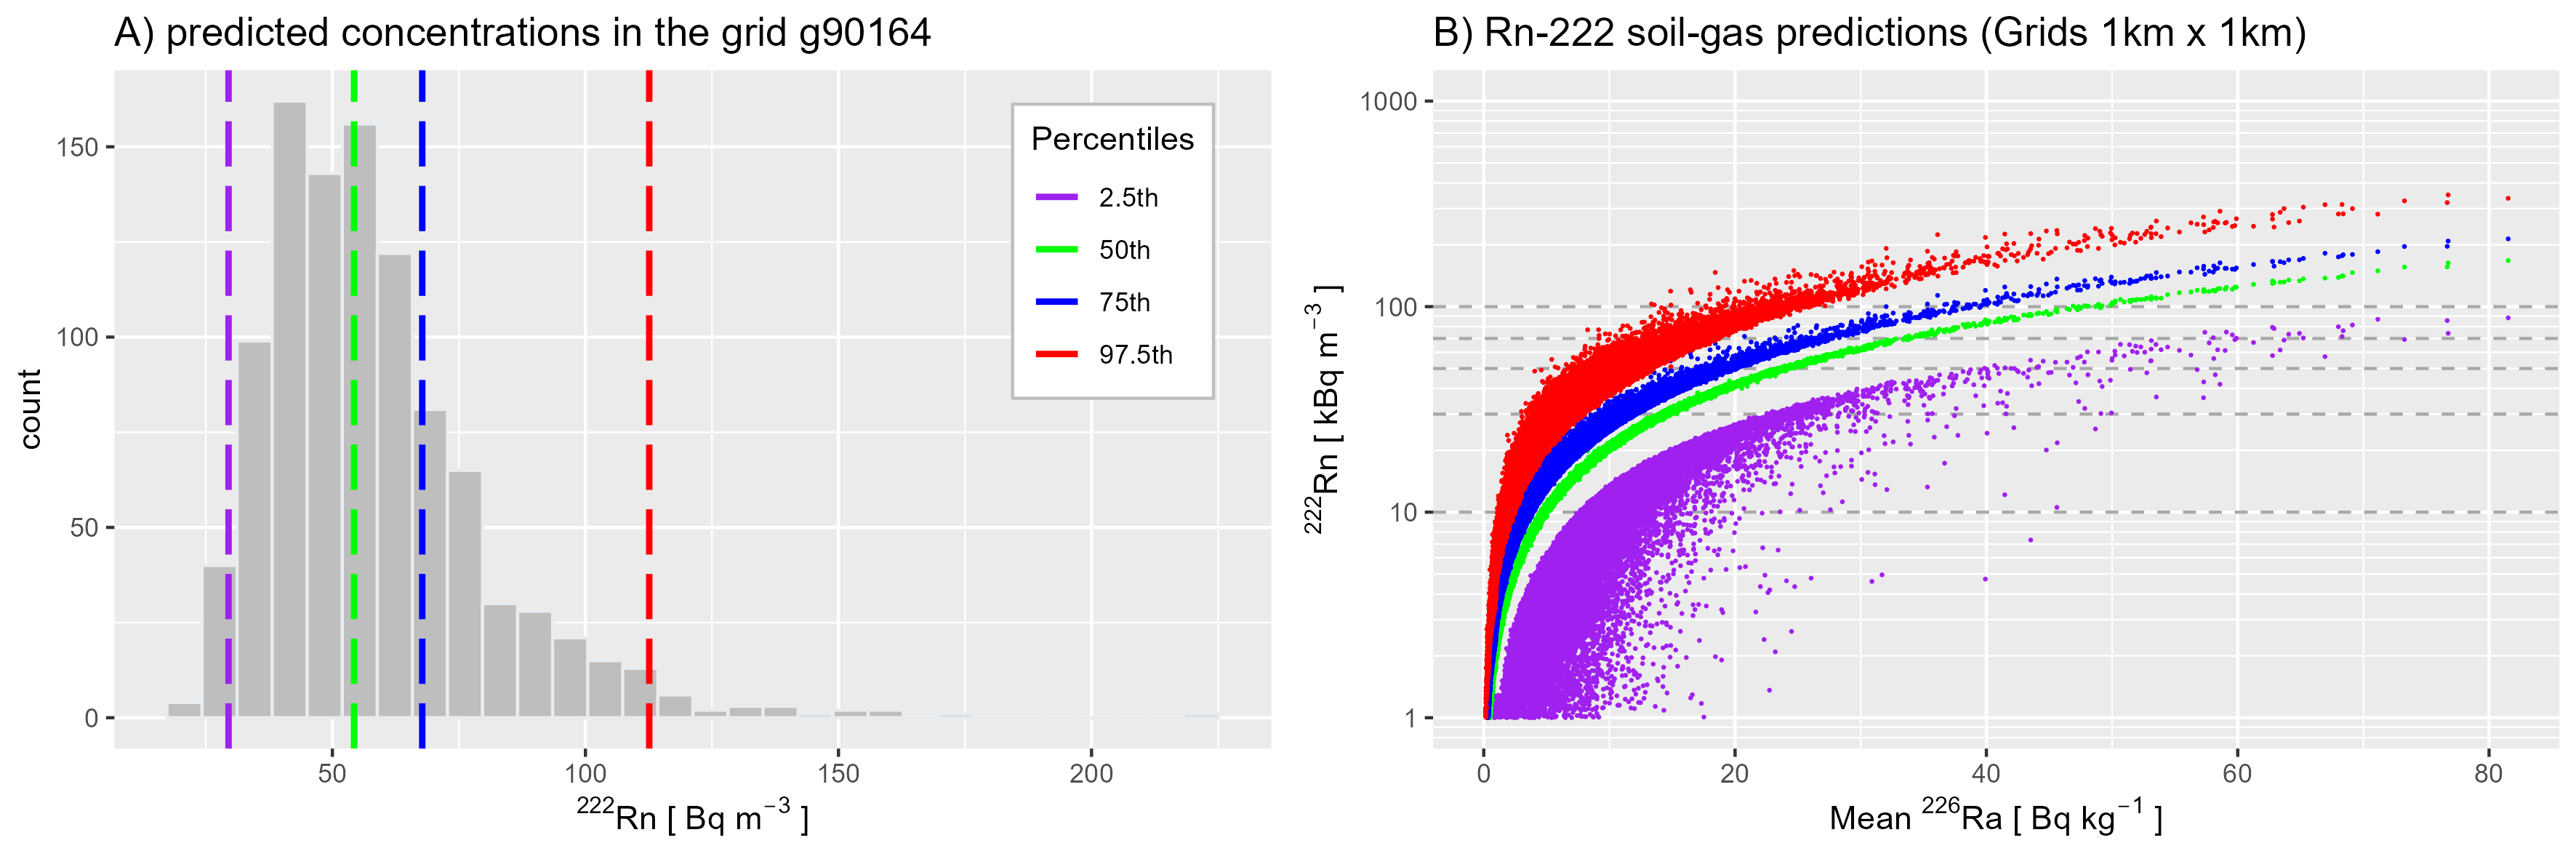
\includegraphics[width=1\linewidth]{Rresults/Figure_1} \end{center}

\hypertarget{figure-2}{%
\subsection{Figure 2}\label{figure-2}}

Equivalent uranium concentration (ppm)

\begin{Shaded}
\begin{Highlighting}[]
  \CommentTok{\#round(BAMMtools::getJenksBreaks(eU\_Grids1km$eU\_AM, 10, subset = NULL), 1)}

\NormalTok{  colpal \textless{}{-}}\StringTok{ }\NormalTok{colorRamps}\OperatorTok{::}\KeywordTok{matlab.like}\NormalTok{(}\DecValTok{9}\NormalTok{)}
  \CommentTok{\#colpal \textless{}{-} viridis::viridis(9)}
  
\NormalTok{  grDevices}\OperatorTok{::}\KeywordTok{png}\NormalTok{(}\StringTok{"Rresults/Figure\_2a.png"}\NormalTok{,}
                 \DataTypeTok{width  =} \DecValTok{550}\NormalTok{,}
                 \DataTypeTok{height =} \DecValTok{650}\NormalTok{,}
                 \DataTypeTok{unit =} \StringTok{"px"}\NormalTok{) }

\NormalTok{  nf \textless{}{-}}\StringTok{ }\KeywordTok{layout}\NormalTok{(}\KeywordTok{matrix}\NormalTok{(}\DecValTok{1}\OperatorTok{:}\DecValTok{2}\NormalTok{, }\DataTypeTok{ncol =} \DecValTok{2}\NormalTok{), }\DataTypeTok{widths =} \KeywordTok{c}\NormalTok{(}\FloatTok{0.8}\NormalTok{, }\KeywordTok{lcm}\NormalTok{(}\DecValTok{2}\NormalTok{)))}
\NormalTok{ \{brks \textless{}{-}}\StringTok{ }\KeywordTok{c}\NormalTok{(}\FloatTok{0.0}\NormalTok{, }\FloatTok{0.3}\NormalTok{, }\FloatTok{0.5}\NormalTok{, }\FloatTok{0.7}\NormalTok{, }\FloatTok{0.9}\NormalTok{, }\FloatTok{1.2}\NormalTok{, }\FloatTok{1.6}\NormalTok{, }\FloatTok{2.3}\NormalTok{, }\FloatTok{3.6}\NormalTok{, }\FloatTok{10.2}\NormalTok{)}
   \KeywordTok{plot}\NormalTok{(}\KeywordTok{st\_geometry}\NormalTok{(Ireland),}
        \DataTypeTok{reset =} \OtherTok{FALSE}\NormalTok{,}
        \DataTypeTok{main =} \StringTok{"a) eU [ppm] {-} Resolution 50m"}\NormalTok{)}
   \KeywordTok{plot}\NormalTok{(eU\_50m,}
         \DataTypeTok{main =} \StringTok{""}\NormalTok{,}
         \DataTypeTok{col =}\NormalTok{ colpal, }
         \DataTypeTok{breaks =}\NormalTok{ brks,}
         \DataTypeTok{at =}\NormalTok{ brks,}
         \DataTypeTok{add =} \OtherTok{TRUE}\NormalTok{,}
         \DataTypeTok{reset =} \OtherTok{FALSE}\NormalTok{,}
\NormalTok{         )}
   \KeywordTok{.image\_scale}\NormalTok{(brks,}
               \DataTypeTok{col =}\NormalTok{ colpal, }
               \DataTypeTok{key.length =} \KeywordTok{lcm}\NormalTok{(}\DecValTok{10}\NormalTok{),}
               \DataTypeTok{key.pos =} \DecValTok{4}\NormalTok{,}
               \DataTypeTok{breaks =}\NormalTok{ brks,}
               \DataTypeTok{at =}\NormalTok{ brks, }
               \DataTypeTok{add.axis =}\NormalTok{ F)}
  \KeywordTok{axis}\NormalTok{(}\DecValTok{4}\NormalTok{,}\DataTypeTok{at =}\NormalTok{ brks, }\DataTypeTok{las =} \DecValTok{2}\NormalTok{, }\DataTypeTok{cex.axis =} \FloatTok{0.75}\NormalTok{)}
\NormalTok{  \}}
  \KeywordTok{dev.off}\NormalTok{()}
  
\NormalTok{  grDevices}\OperatorTok{::}\KeywordTok{png}\NormalTok{(}\StringTok{"Rresults/Figure\_2b.png"}\NormalTok{,}
                 \DataTypeTok{width  =} \DecValTok{550}\NormalTok{,}
                 \DataTypeTok{height =} \DecValTok{650}\NormalTok{,}
                 \DataTypeTok{unit =} \StringTok{"px"}\NormalTok{) }
  
\NormalTok{  nf \textless{}{-}}\StringTok{ }\KeywordTok{layout}\NormalTok{(}\KeywordTok{matrix}\NormalTok{(}\DecValTok{1}\OperatorTok{:}\DecValTok{2}\NormalTok{, }\DataTypeTok{ncol =} \DecValTok{2}\NormalTok{), }\DataTypeTok{widths =} \KeywordTok{c}\NormalTok{(}\FloatTok{0.8}\NormalTok{, }\KeywordTok{lcm}\NormalTok{(}\DecValTok{2}\NormalTok{)))}
\NormalTok{  \{brks \textless{}{-}}\StringTok{ }\KeywordTok{c}\NormalTok{(}\FloatTok{0.0}\NormalTok{, }\FloatTok{0.3}\NormalTok{, }\FloatTok{0.5}\NormalTok{, }\FloatTok{0.7}\NormalTok{, }\FloatTok{0.9}\NormalTok{, }\FloatTok{1.2}\NormalTok{, }\FloatTok{1.6}\NormalTok{, }\FloatTok{2.3}\NormalTok{, }\FloatTok{3.6}\NormalTok{, }\FloatTok{6.7}\NormalTok{)}
  \KeywordTok{plot}\NormalTok{(}\KeywordTok{st\_geometry}\NormalTok{(Ireland),}
       \DataTypeTok{reset =} \OtherTok{FALSE}\NormalTok{, }
       \DataTypeTok{main =} \StringTok{"b) eU [ppm] {-} Resolution 1km"}\NormalTok{,)}
  \KeywordTok{plot}\NormalTok{(eU\_Grids1km[}\StringTok{"eU\_AM"}\NormalTok{], }\DataTypeTok{border=}\OtherTok{NA}\NormalTok{,}
       \DataTypeTok{main =} \StringTok{""}\NormalTok{,}
       \DataTypeTok{pal =}\NormalTok{ colpal, }
       \DataTypeTok{breaks =}\NormalTok{ brks,}
       \DataTypeTok{at =}\NormalTok{ brks,}
       \DataTypeTok{add =} \OtherTok{TRUE}\NormalTok{,}
       \DataTypeTok{reset =} \OtherTok{FALSE}\NormalTok{,}
\NormalTok{       )}
  \KeywordTok{.image\_scale}\NormalTok{(brks,}
               \DataTypeTok{col =}\NormalTok{ colpal, }
               \DataTypeTok{key.length =} \KeywordTok{lcm}\NormalTok{(}\DecValTok{10}\NormalTok{),}
               \DataTypeTok{key.pos =} \DecValTok{4}\NormalTok{,}
               \DataTypeTok{breaks =}\NormalTok{ brks,}
               \DataTypeTok{at =}\NormalTok{ brks, }
               \DataTypeTok{add.axis =} \OtherTok{FALSE}\NormalTok{)}
  \KeywordTok{axis}\NormalTok{(}\DecValTok{4}\NormalTok{,}\DataTypeTok{at =}\NormalTok{ brks, }\DataTypeTok{las =} \DecValTok{2}\NormalTok{, }\DataTypeTok{cex.axis =} \FloatTok{0.75}\NormalTok{)}
\NormalTok{  \}}
  \KeywordTok{dev.off}\NormalTok{()}
\end{Highlighting}
\end{Shaded}

\begin{center}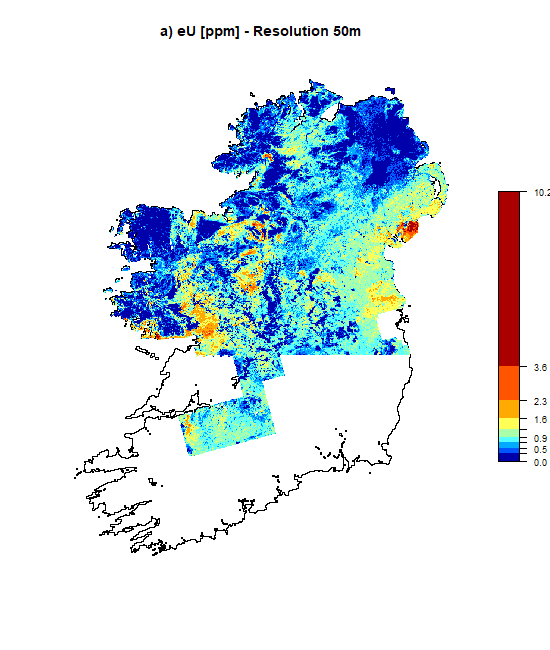
\includegraphics[width=0.5\linewidth]{Rresults/Figure_2a} \end{center}

\begin{center}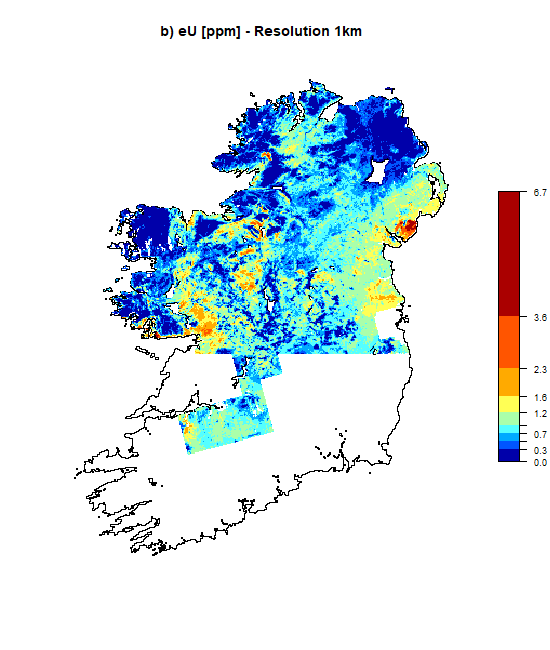
\includegraphics[width=0.5\linewidth]{Rresults/Figure_2b} \end{center}

\hypertarget{figure-3}{%
\subsection{Figure 3}\label{figure-3}}

Subsoil permeability map of the island of Ireland (based on the
All-Ireland Quaternary map)

\begin{Shaded}
\begin{Highlighting}[]
\NormalTok{  Karst \textless{}{-}}\StringTok{ }\NormalTok{Karst }\OperatorTok{\%\textgreater{}\%}\StringTok{ }\KeywordTok{mutate}\NormalTok{(}\DataTypeTok{Bedrock =} \KeywordTok{if\_else}\NormalTok{(Karst }\OperatorTok{==}\StringTok{ }\OtherTok{TRUE}\NormalTok{,}
                                              \StringTok{"Bedrock (Karstified)"}\NormalTok{,}
                                              \StringTok{"Bedrock (No Karstified)"}\NormalTok{))}
  
\NormalTok{  QG\_Colors \textless{}{-}}\StringTok{ }\KeywordTok{c}\NormalTok{(}\StringTok{"Bedrock (Karstified)"}\NormalTok{    =}\StringTok{ "darkgrey"}\NormalTok{,}
                 \StringTok{"Bedrock (No Karstified)"}\NormalTok{ =}\StringTok{ "lightgrey"}\NormalTok{,}
                 \StringTok{"Alluvium"}\NormalTok{ =}\StringTok{ "\#ffff89"}\NormalTok{,}
                 \StringTok{"Glaciofluvial/glaciolacustrine sand and gravel"}\NormalTok{ =}\StringTok{ "\#CCCC33"}\NormalTok{,}
                 \StringTok{"Glaciomarine sediments"}\NormalTok{ =}\StringTok{ "\#CC0000"}\NormalTok{,}
                 \StringTok{"Lacustrine sediments"}\NormalTok{ =}\StringTok{ "yellow"}\NormalTok{,}
                 \StringTok{"Marine and estuarine deposits"}\NormalTok{ =}\StringTok{ "\#f4efe4"}\NormalTok{,}
                 \StringTok{"Peat"}\NormalTok{ =}\StringTok{ "\#ac7f50"}\NormalTok{,}
                 \StringTok{"Slope deposits"}\NormalTok{ =}\StringTok{ "\#996699"}\NormalTok{,}
                 \StringTok{"Till derived from acidic volcanic rocks"}\NormalTok{ =}\StringTok{ "\#FF9999"}\NormalTok{,}
                 \StringTok{"Till derived from basic igneous rocks"}\NormalTok{ =}\StringTok{ "\#ffc1b7"}\NormalTok{,}
                 \StringTok{"Till derived from Devonian sandstones"}\NormalTok{ =}\StringTok{ "\#CD5C5C"}\NormalTok{,}
                 \StringTok{"Till derived from granites"}\NormalTok{ =}\StringTok{ "\#ff3317"}\NormalTok{,}
                 \StringTok{"Till derived from limestones"}\NormalTok{ =}\StringTok{ "\#bddbf1"}\NormalTok{,}
                 \StringTok{"Till derived from metamorphic rocks"}\NormalTok{ =}\StringTok{ "\#a7a7ff"}\NormalTok{,}
                 \StringTok{"Till derived from sandstones"}\NormalTok{ =}\StringTok{ "\#ffcb23"}\NormalTok{,}
                 \StringTok{"Till derived from sandstones and shales"}\NormalTok{ =}\StringTok{ "\#888888"}\NormalTok{,}
                 \StringTok{"Wind blown sand"}\NormalTok{ =}\StringTok{ "\#f1e5df"} 
\NormalTok{  )}
                  
\NormalTok{  p1 \textless{}{-}}\StringTok{ }\KeywordTok{ggplot}\NormalTok{() }\OperatorTok{+}
\StringTok{    }\KeywordTok{geom\_sf}\NormalTok{(}\DataTypeTok{data =}\NormalTok{ Karst, }\KeywordTok{aes}\NormalTok{(}\DataTypeTok{fill =}\NormalTok{ Bedrock), }\DataTypeTok{colour =} \OtherTok{NA}\NormalTok{) }\OperatorTok{+}
\StringTok{    }\KeywordTok{geom\_sf}\NormalTok{(}\DataTypeTok{data =}\NormalTok{ QG, }\KeywordTok{aes}\NormalTok{(}\DataTypeTok{fill =}\NormalTok{ Sediment\_}\DecValTok{5}\NormalTok{), }\DataTypeTok{colour =} \OtherTok{NA}\NormalTok{) }\OperatorTok{+}
\StringTok{    }\KeywordTok{scale\_fill\_manual}\NormalTok{(}\DataTypeTok{name =} \StringTok{"Deposits"}\NormalTok{, }\DataTypeTok{values =}\NormalTok{ QG\_Colors) }\OperatorTok{+}
\StringTok{    }\KeywordTok{ggtitle}\NormalTok{(}\StringTok{"All Ireland Quaternary Map 500k"}\NormalTok{) }

\NormalTok{  p2 \textless{}{-}}\StringTok{ }\KeywordTok{ggplot}\NormalTok{() }\OperatorTok{+}
\StringTok{    }\KeywordTok{geom\_sf}\NormalTok{(}\DataTypeTok{data =}\NormalTok{ SP, }\KeywordTok{aes}\NormalTok{(}\DataTypeTok{fill =}\NormalTok{ Perm), }\DataTypeTok{colour =} \OtherTok{NA}\NormalTok{) }\OperatorTok{+}
\StringTok{    }\KeywordTok{scale\_fill\_manual}\NormalTok{(}\DataTypeTok{name =} \StringTok{"Perm"}\NormalTok{, }
                      \DataTypeTok{labels =} \KeywordTok{c}\NormalTok{(}\StringTok{"High"}\NormalTok{, }\StringTok{"Moderate"}\NormalTok{, }\StringTok{"Low"}\NormalTok{),}
                      \DataTypeTok{values =} \KeywordTok{c}\NormalTok{(}\StringTok{"red"}\NormalTok{, }\StringTok{"yellow3"}\NormalTok{, }\StringTok{"blue"}\NormalTok{)) }\OperatorTok{+}
\StringTok{    }\KeywordTok{ggtitle}\NormalTok{(}\StringTok{"Subsoil permeability based on GW, QG and AT"}\NormalTok{) }

  \KeywordTok{ggsave}\NormalTok{(}\DataTypeTok{file =} \StringTok{"Rresults/Figure\_3.png"}\NormalTok{,}
\NormalTok{         gridExtra}\OperatorTok{::}\KeywordTok{arrangeGrob}\NormalTok{(p1, p2, }\DataTypeTok{nrow =} \DecValTok{1}\NormalTok{),}
       \DataTypeTok{width =} \DecValTok{38}\NormalTok{,}
       \DataTypeTok{height =} \DecValTok{14}\NormalTok{,}
       \DataTypeTok{units =} \StringTok{"cm"}\NormalTok{)}
\end{Highlighting}
\end{Shaded}

\begin{center}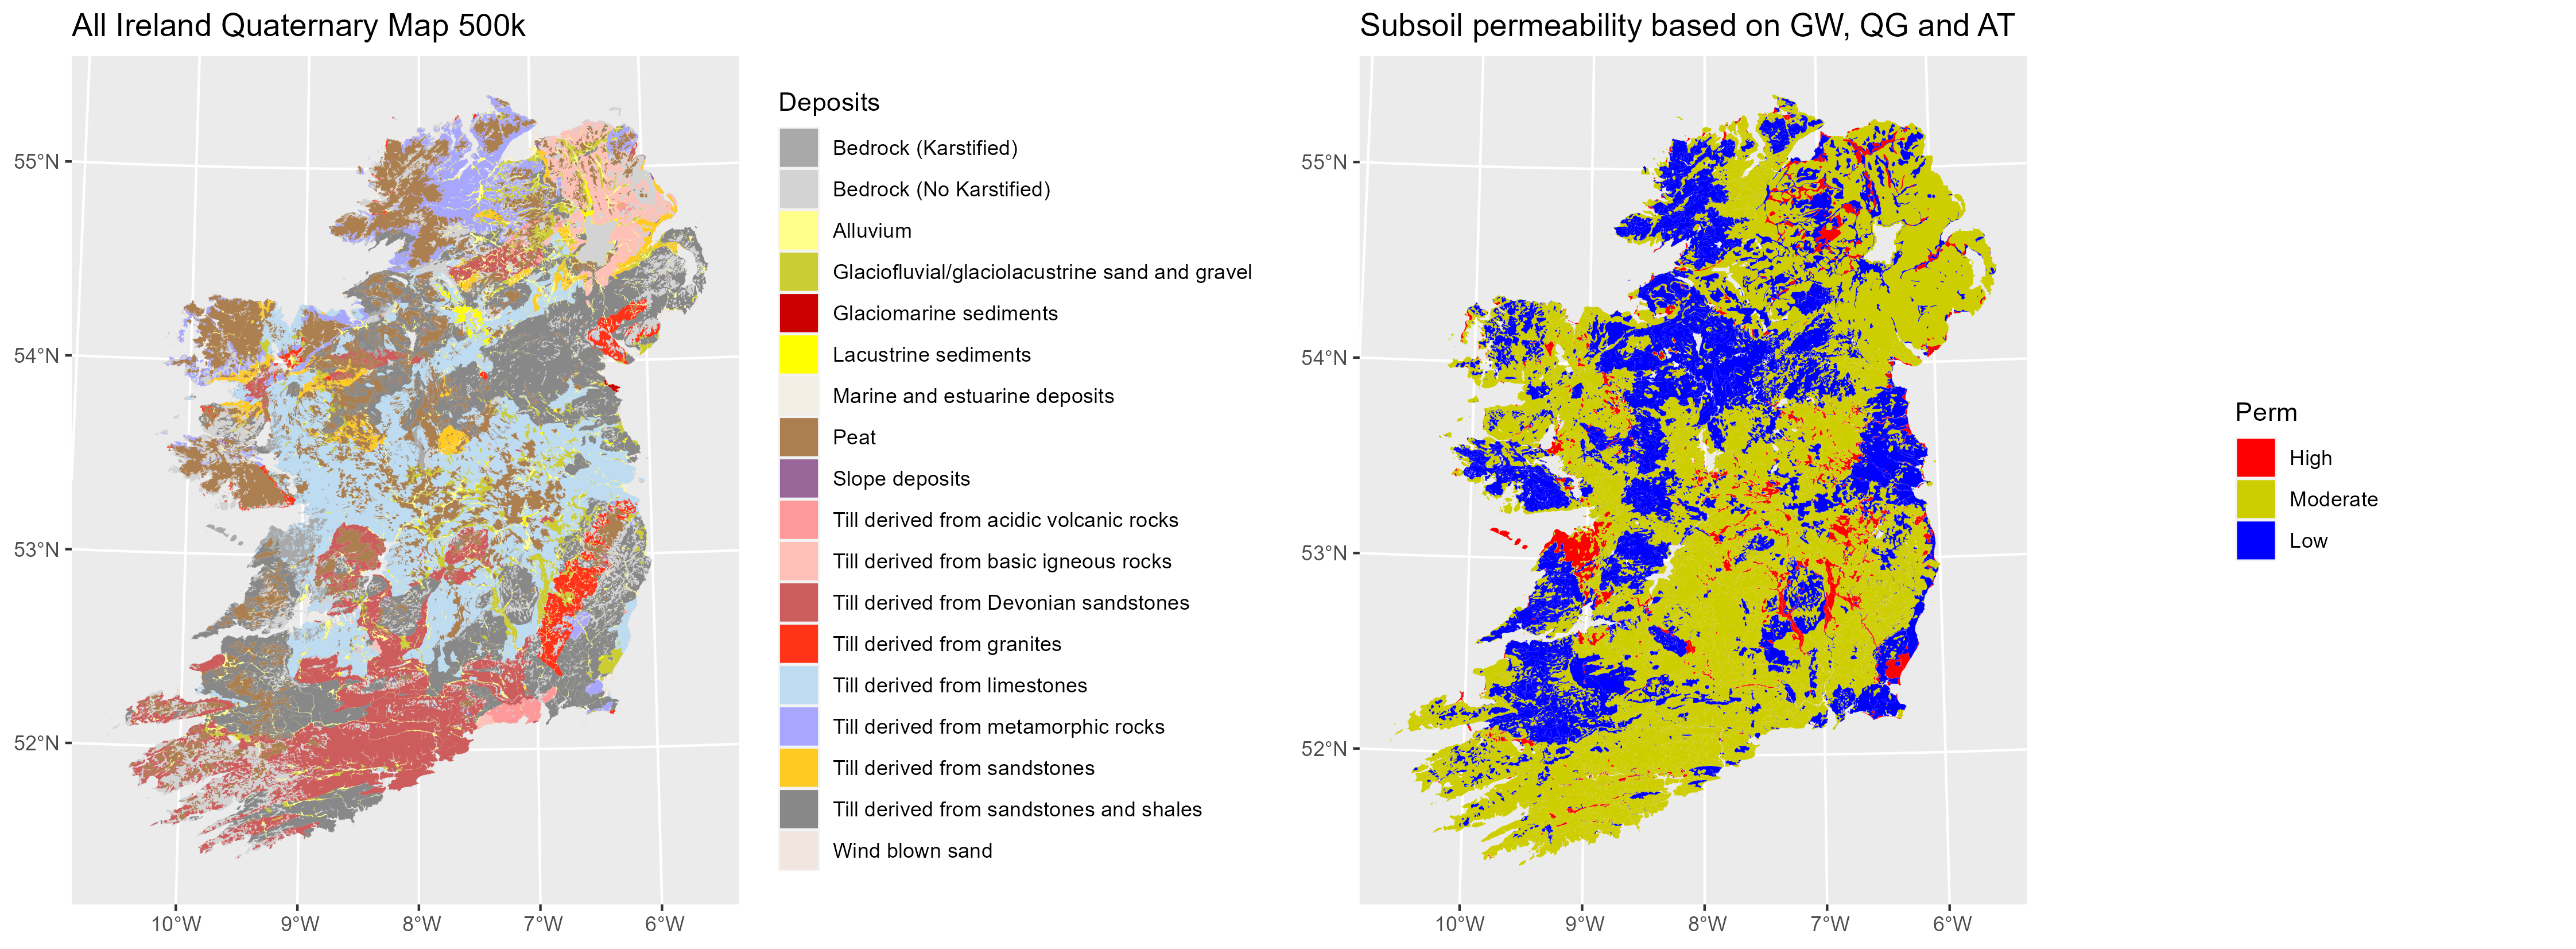
\includegraphics[width=1\linewidth]{Rresults/Figure_3} \end{center}

\hypertarget{figure-4}{%
\subsection{Figure 4:}\label{figure-4}}

Indoor radon measurements from old survey (Jan.~1992 -- Feb.~2013; N =
31,910) and the new survey (Feb.~2013 -- Jul.~2017; N = 6,859). Grey
area: part covered by the Tellus airborne survey illustrated in this
study. Note that no geolocated indoor radon data are available for
Northern Ireland, as these are held by Public Health England and are not
available for this study.

\begin{Shaded}
\begin{Highlighting}[]
\NormalTok{  p1 \textless{}{-}}\StringTok{ }\KeywordTok{ggplot}\NormalTok{() }\OperatorTok{+}
\StringTok{    }\KeywordTok{geom\_sf}\NormalTok{(}\DataTypeTok{data =}\NormalTok{ Ireland) }\OperatorTok{+}
\StringTok{    }\KeywordTok{geom\_sf}\NormalTok{(}\DataTypeTok{data =}\NormalTok{ RP\_Grids, }\DataTypeTok{colour =} \StringTok{"grey"}\NormalTok{) }\OperatorTok{+}
\StringTok{    }\KeywordTok{geom\_sf}\NormalTok{(}\DataTypeTok{data =} \KeywordTok{filter}\NormalTok{(InRn, Survey }\OperatorTok{==}\StringTok{ "Old"}\NormalTok{),}
            \KeywordTok{aes}\NormalTok{(}\DataTypeTok{fill =}\NormalTok{ Case, }\DataTypeTok{color =}\NormalTok{ Case),}
            \DataTypeTok{size =} \FloatTok{0.1}\NormalTok{,}
            \DataTypeTok{alpha =} \FloatTok{0.75}\NormalTok{) }\OperatorTok{+}
\StringTok{    }\KeywordTok{scale\_fill\_manual}\NormalTok{(}\DataTypeTok{name =} \StringTok{"Bq/m3"}\NormalTok{,}
                      \DataTypeTok{labels =} \KeywordTok{c}\NormalTok{(}\StringTok{"\textless{} 200"}\NormalTok{,}
                                 \StringTok{"\textgreater{}= 200"}\NormalTok{),}
                      \DataTypeTok{values =} \KeywordTok{c}\NormalTok{(}\StringTok{"black"}\NormalTok{,}
                                 \StringTok{"red"}\NormalTok{)) }\OperatorTok{+}
\StringTok{    }\KeywordTok{scale\_color\_manual}\NormalTok{(}\DataTypeTok{name =} \StringTok{"Bq/m3"}\NormalTok{,}
                       \DataTypeTok{labels =} \KeywordTok{c}\NormalTok{(}\StringTok{"\textless{} 200"}\NormalTok{,}
                                  \StringTok{"\textgreater{}= 200"}\NormalTok{),}
                       \DataTypeTok{values =} \KeywordTok{c}\NormalTok{(}\StringTok{"black"}\NormalTok{,}
                                  \StringTok{"red"}\NormalTok{)) }\OperatorTok{+}
\StringTok{    }\KeywordTok{guides}\NormalTok{(}\DataTypeTok{colour =} \KeywordTok{guide\_legend}\NormalTok{(}\DataTypeTok{override.aes =} \KeywordTok{list}\NormalTok{(}\DataTypeTok{size =} \DecValTok{2}\NormalTok{))) }\OperatorTok{+}
\StringTok{    }\KeywordTok{labs}\NormalTok{(}\DataTypeTok{title =} \StringTok{"Period Jan. 1992 {-} Feb. 2013"}\NormalTok{) }

\NormalTok{  p2 \textless{}{-}}\StringTok{ }\KeywordTok{ggplot}\NormalTok{() }\OperatorTok{+}
\StringTok{    }\KeywordTok{geom\_sf}\NormalTok{(}\DataTypeTok{data =}\NormalTok{ Ireland) }\OperatorTok{+}
\StringTok{    }\KeywordTok{geom\_sf}\NormalTok{(}\DataTypeTok{data =}\NormalTok{ RP\_Grids, }\DataTypeTok{colour =} \StringTok{"grey"}\NormalTok{) }\OperatorTok{+}
\StringTok{    }\KeywordTok{geom\_sf}\NormalTok{(}\DataTypeTok{data =} \KeywordTok{filter}\NormalTok{(InRn, Survey }\OperatorTok{==}\StringTok{ "New"}\NormalTok{),}
            \KeywordTok{aes}\NormalTok{(}\DataTypeTok{fill =}\NormalTok{ Case, }\DataTypeTok{color =}\NormalTok{ Case),}
            \DataTypeTok{size =} \FloatTok{0.1}\NormalTok{,}
            \DataTypeTok{alpha =} \FloatTok{0.75}\NormalTok{) }\OperatorTok{+}
\StringTok{    }\KeywordTok{scale\_fill\_manual}\NormalTok{(}\DataTypeTok{name =} \StringTok{"Bq/m3"}\NormalTok{,}
                      \DataTypeTok{labels =} \KeywordTok{c}\NormalTok{(}\StringTok{"\textless{} 200"}\NormalTok{,}
                                 \StringTok{"\textgreater{}= 200"}\NormalTok{),}
                      \DataTypeTok{values =} \KeywordTok{c}\NormalTok{(}\StringTok{"black"}\NormalTok{,}
                                 \StringTok{"red"}\NormalTok{)) }\OperatorTok{+}
\StringTok{    }\KeywordTok{scale\_color\_manual}\NormalTok{(}\DataTypeTok{name =} \StringTok{"Bq/m3"}\NormalTok{,}
                       \DataTypeTok{labels =} \KeywordTok{c}\NormalTok{(}\StringTok{"\textless{} 200"}\NormalTok{,}
                                  \StringTok{"\textgreater{}= 200"}\NormalTok{),}
                       \DataTypeTok{values =} \KeywordTok{c}\NormalTok{(}\StringTok{"black"}\NormalTok{,}
                                  \StringTok{"red"}\NormalTok{)) }\OperatorTok{+}
\StringTok{    }\KeywordTok{guides}\NormalTok{(}\DataTypeTok{colour =} \KeywordTok{guide\_legend}\NormalTok{(}\DataTypeTok{override.aes =} \KeywordTok{list}\NormalTok{(}\DataTypeTok{size =} \DecValTok{2}\NormalTok{))) }\OperatorTok{+}
\StringTok{    }\KeywordTok{labs}\NormalTok{(}\DataTypeTok{title =} \StringTok{"Period Feb. 2013 {-} Jul. 2017"}\NormalTok{)  }

  \KeywordTok{ggsave}\NormalTok{(}\DataTypeTok{file =} \StringTok{"Rresults/Figure\_4.png"}\NormalTok{,}
\NormalTok{         gridExtra}\OperatorTok{::}\KeywordTok{arrangeGrob}\NormalTok{(p1, p2, }\DataTypeTok{nrow =} \DecValTok{1}\NormalTok{),}
         \DataTypeTok{width =} \DecValTok{28}\NormalTok{,}
         \DataTypeTok{height =} \DecValTok{14}\NormalTok{,}
         \DataTypeTok{units =} \StringTok{"cm"}\NormalTok{ )}
\end{Highlighting}
\end{Shaded}

\begin{center}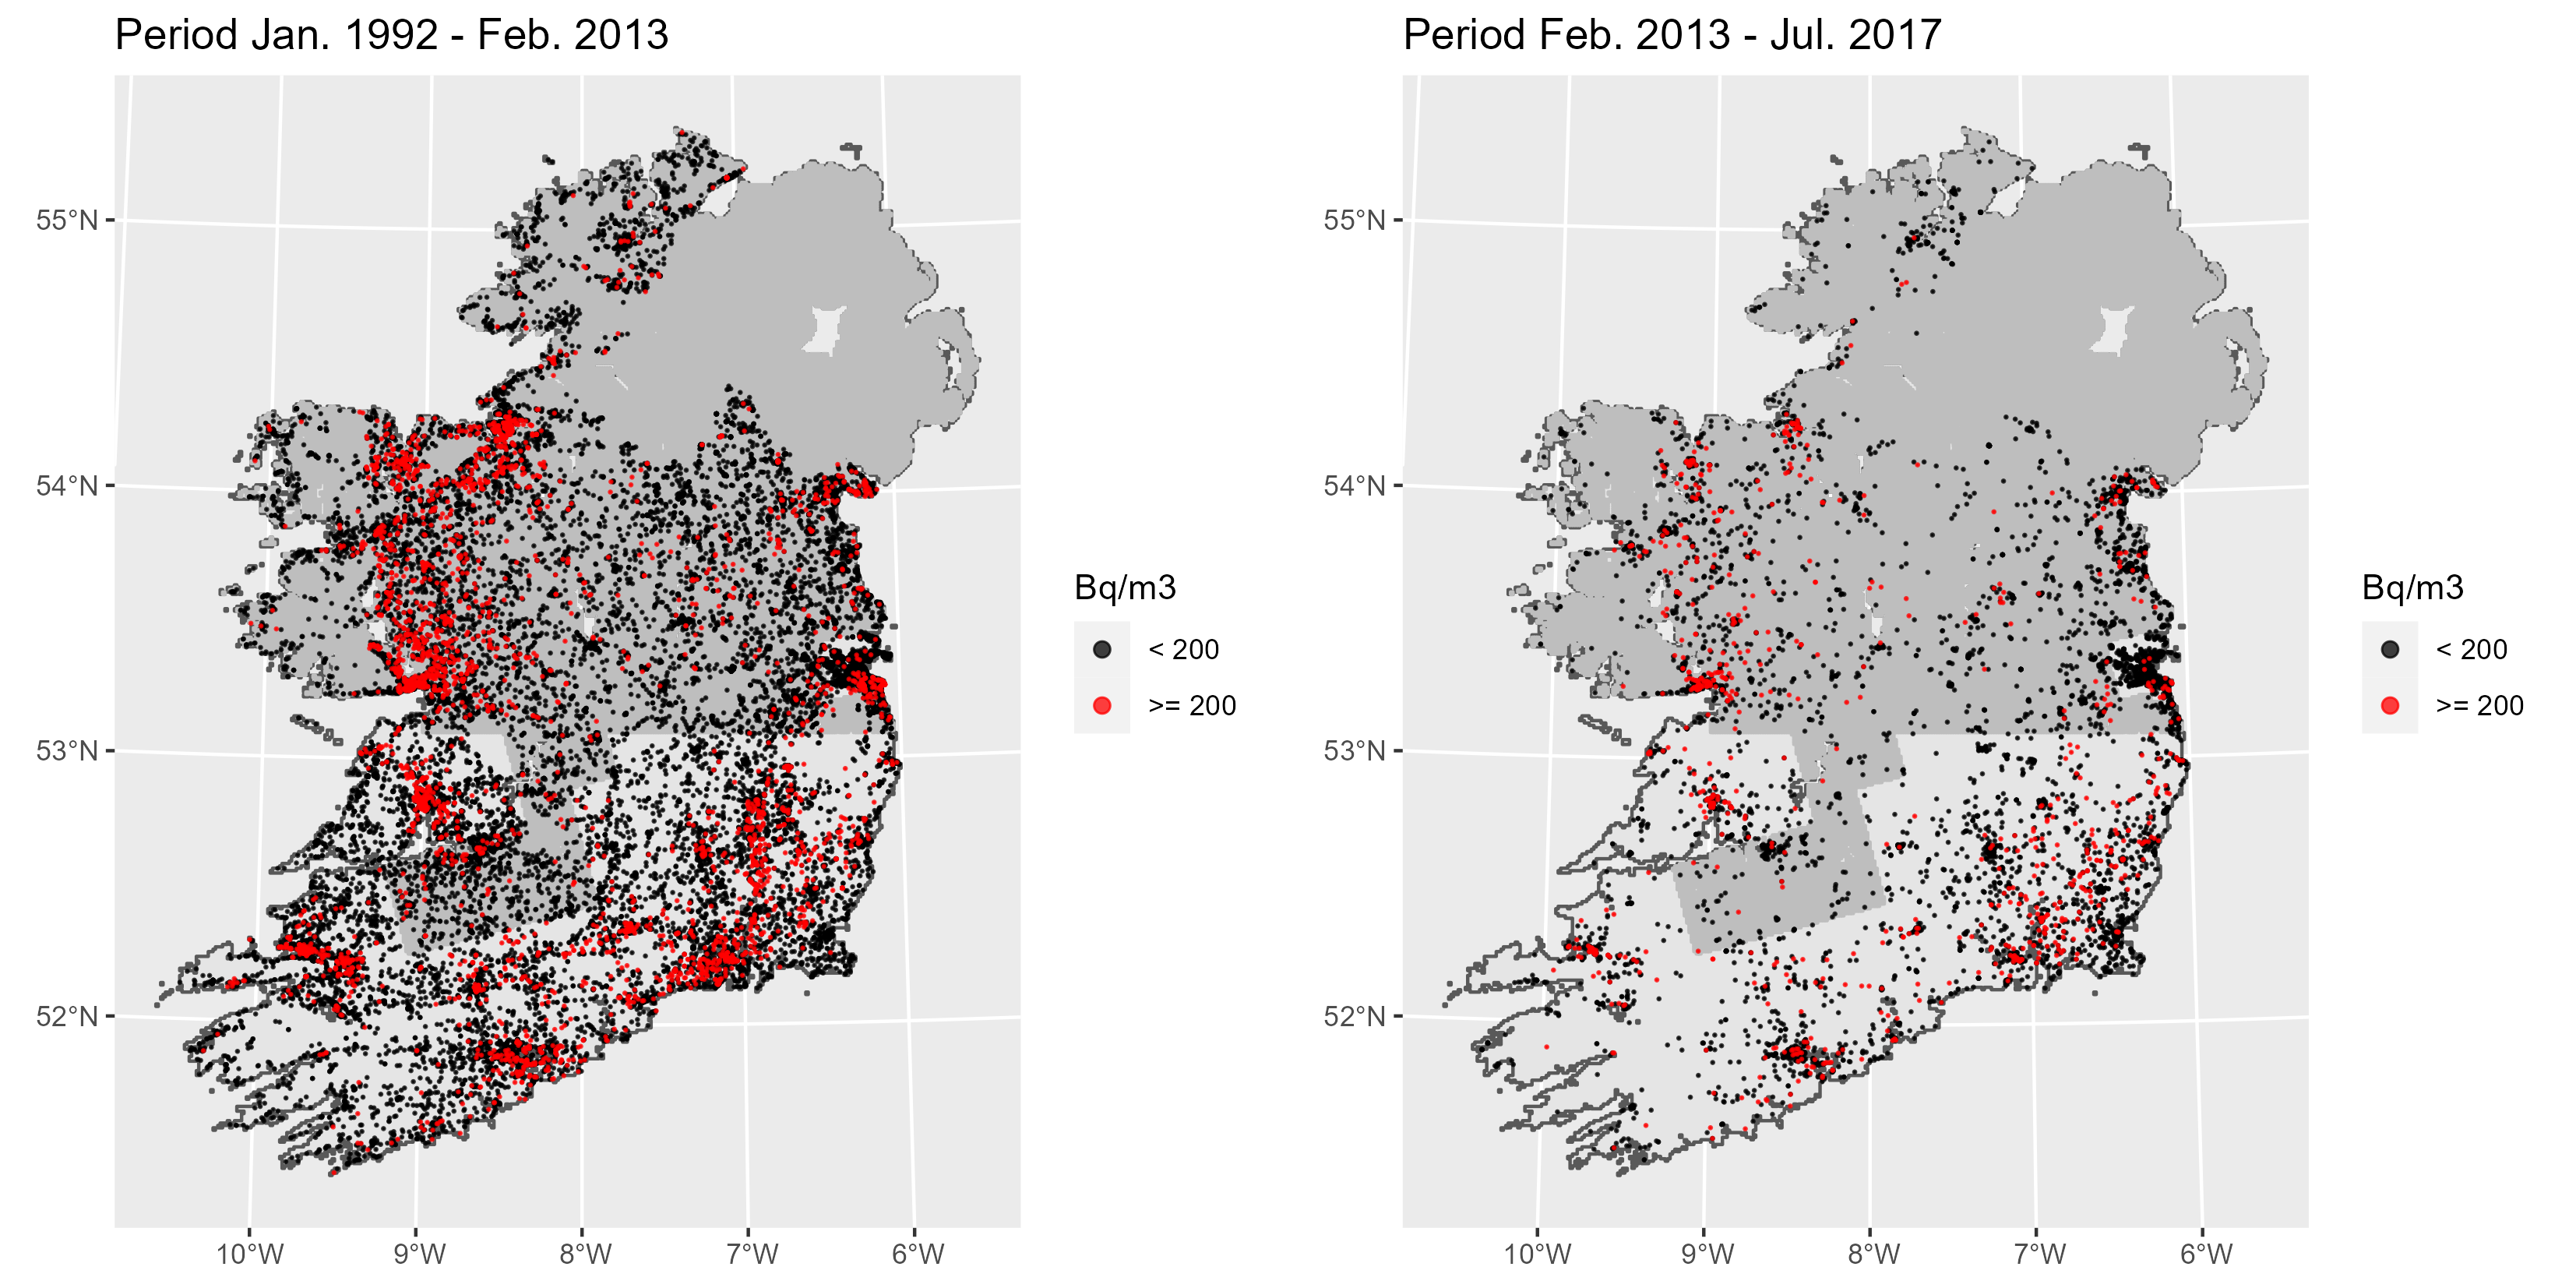
\includegraphics[width=0.85\linewidth]{Rresults/Figure_4} \end{center}

\hypertarget{figure-5}{%
\subsection{Figure 5}\label{figure-5}}

Radon soil-gas classification based on airborne radiometrics

\begin{Shaded}
\begin{Highlighting}[]
\NormalTok{  Col\_Ramp \textless{}{-}}\StringTok{ }\NormalTok{RColorBrewer}\OperatorTok{::}\KeywordTok{brewer.pal}\NormalTok{(}\DecValTok{6}\NormalTok{, }\StringTok{"Spectral"}\NormalTok{)}
\NormalTok{  p1 \textless{}{-}}\StringTok{ }\KeywordTok{ggplot}\NormalTok{() }\OperatorTok{+}\StringTok{ }
\StringTok{    }\KeywordTok{geom\_sf}\NormalTok{(}\DataTypeTok{data =}\NormalTok{ Ireland) }\OperatorTok{+}
\StringTok{    }\KeywordTok{geom\_sf}\NormalTok{(}\DataTypeTok{data =}\NormalTok{ eU\_Grids1km, }\KeywordTok{aes}\NormalTok{(}\DataTypeTok{fill =}\NormalTok{ Rn\_class), }\DataTypeTok{colour =} \OtherTok{NA}\NormalTok{) }\OperatorTok{+}
\StringTok{    }\KeywordTok{scale\_fill\_manual}\NormalTok{(}\DataTypeTok{name =} \StringTok{"Rn Class"}\NormalTok{,}
                      \DataTypeTok{values =}\NormalTok{ Col\_Ramp) }\OperatorTok{+}
\StringTok{    }\KeywordTok{ggtitle}\NormalTok{(}\StringTok{"Radon soil{-}gas classification based on airborne radiometrics"}\NormalTok{) }
 
  \KeywordTok{ggsave}\NormalTok{(p1,}
         \DataTypeTok{file =} \StringTok{"Rresults/Figure\_5.png"}\NormalTok{,}
         \DataTypeTok{width =} \DecValTok{14}\NormalTok{,}
         \DataTypeTok{height =} \DecValTok{14}\NormalTok{,}
         \DataTypeTok{units =} \StringTok{"cm"}\NormalTok{ )}
\end{Highlighting}
\end{Shaded}

\begin{center}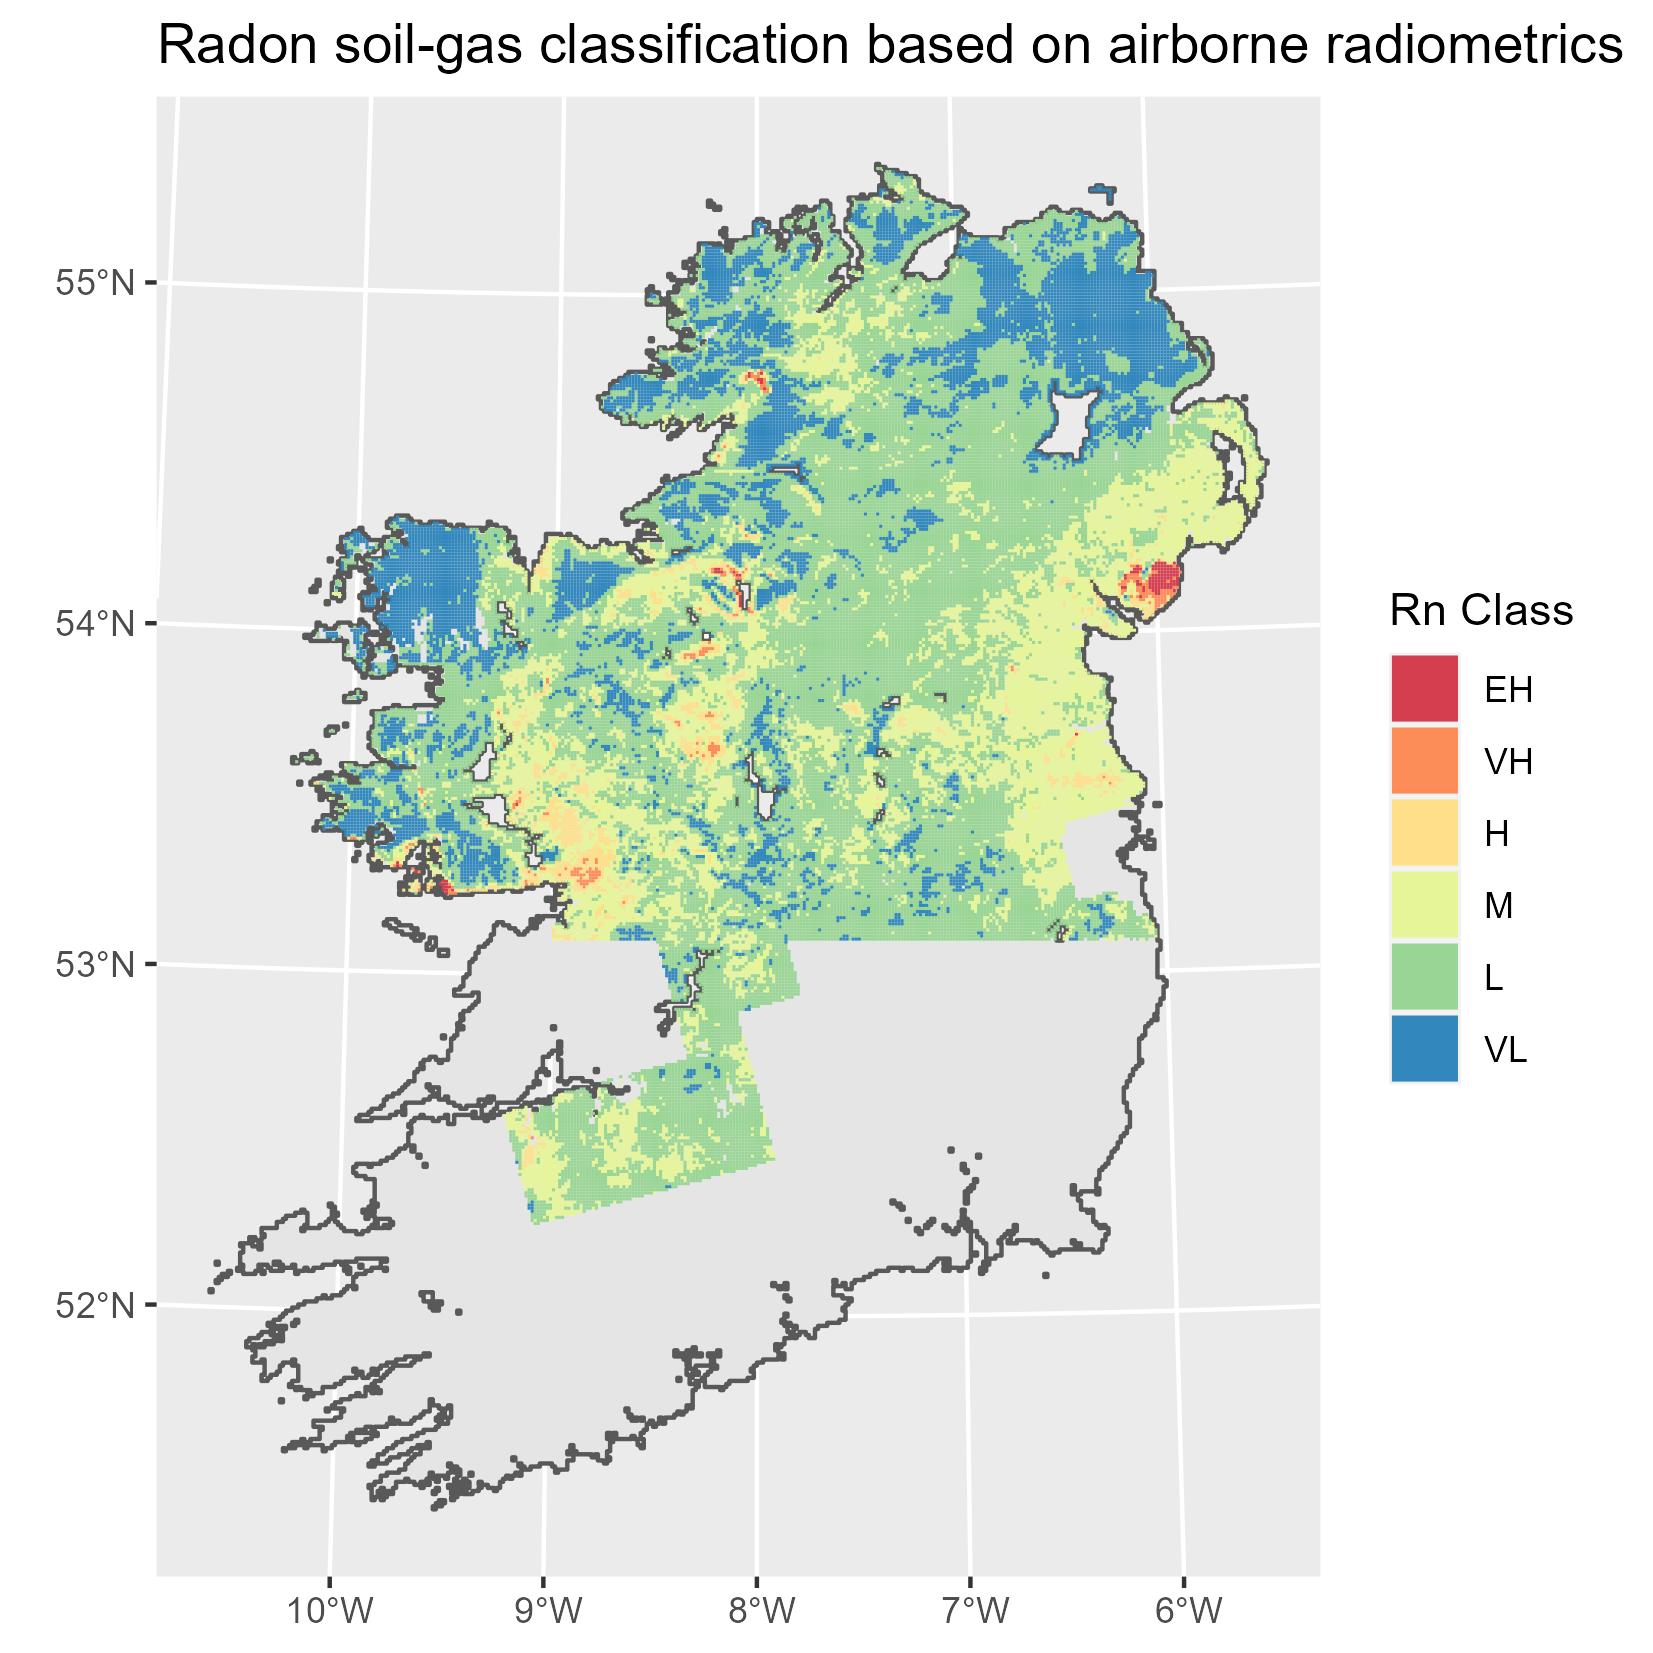
\includegraphics[width=0.5\linewidth]{Rresults/Figure_5} \end{center}

\hypertarget{figure-6}{%
\subsection{Figure 6}\label{figure-6}}

Radon Potential map based on gamma-ray spectrometry airborne
radiometrics and subsoil permeability

\begin{Shaded}
\begin{Highlighting}[]
\NormalTok{  Col\_Ramp \textless{}{-}}\StringTok{ }\NormalTok{RColorBrewer}\OperatorTok{::}\KeywordTok{brewer.pal}\NormalTok{(}\DecValTok{4}\NormalTok{, }\StringTok{"Spectral"}\NormalTok{)}
\NormalTok{  p1 \textless{}{-}}\StringTok{ }\KeywordTok{ggplot}\NormalTok{() }\OperatorTok{+}\StringTok{ }
\StringTok{    }\KeywordTok{geom\_sf}\NormalTok{(}\DataTypeTok{data =}\NormalTok{ Ireland) }\OperatorTok{+}
\StringTok{    }\KeywordTok{geom\_sf}\NormalTok{(}\DataTypeTok{data =}\NormalTok{ RP\_Grids, }\KeywordTok{aes}\NormalTok{(}\DataTypeTok{fill =}\NormalTok{ RP\_class), }\DataTypeTok{colour =} \OtherTok{NA}\NormalTok{) }\OperatorTok{+}
\StringTok{    }\KeywordTok{scale\_fill\_manual}\NormalTok{(}\DataTypeTok{name =} \StringTok{"GRP Class"}\NormalTok{,}
                      \DataTypeTok{values =}\NormalTok{ Col\_Ramp) }\OperatorTok{+}
\StringTok{    }\KeywordTok{ggtitle}\NormalTok{(}\StringTok{"Radon Potential map based on airborne radiometrics"}\NormalTok{) }
  
   \KeywordTok{ggsave}\NormalTok{(p1,}
          \DataTypeTok{file =} \StringTok{"Rresults/Figure\_6.png"}\NormalTok{,}
         \DataTypeTok{width =} \DecValTok{14}\NormalTok{,}
         \DataTypeTok{height =} \DecValTok{14}\NormalTok{,}
         \DataTypeTok{units =} \StringTok{"cm"}\NormalTok{ )}
\end{Highlighting}
\end{Shaded}

\begin{center}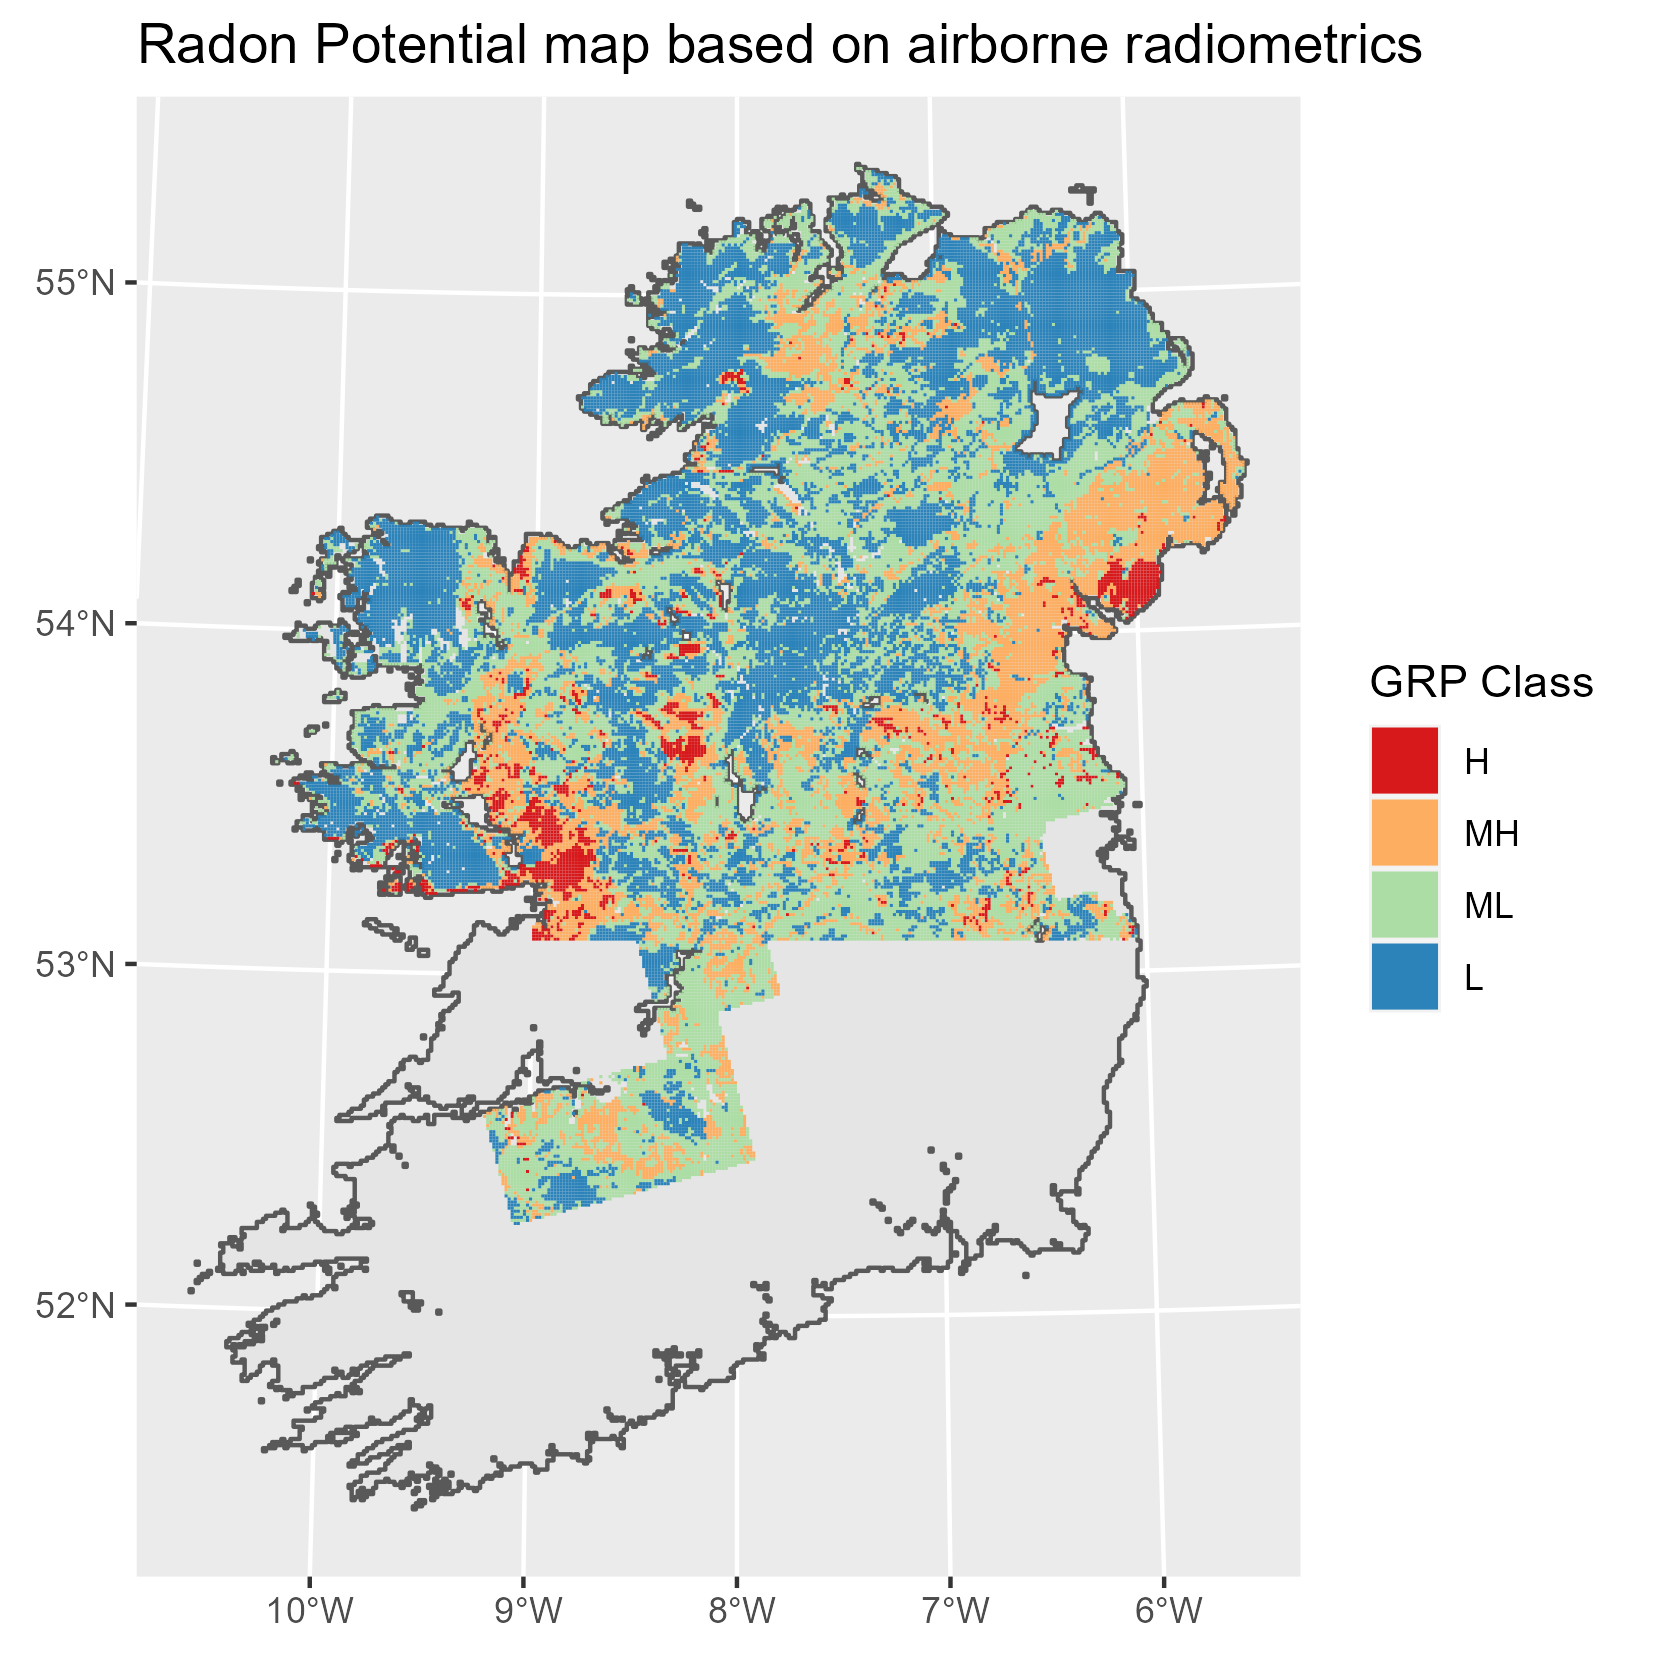
\includegraphics[width=0.5\linewidth]{Rresults/Figure_6} \end{center}

\hypertarget{figure-7}{%
\subsection{Figure 7}\label{figure-7}}

Histogram and probability plot of the new and old indoor radon
measurements

\begin{Shaded}
\begin{Highlighting}[]
\NormalTok{  df\_New \textless{}{-}}\StringTok{ }\KeywordTok{as.data.frame}\NormalTok{(}\KeywordTok{qqnorm}\NormalTok{(}\KeywordTok{log10}\NormalTok{(InRn[InRn}\OperatorTok{$}\NormalTok{Survey}\OperatorTok{==}\StringTok{"New"}\NormalTok{,]}\OperatorTok{$}\NormalTok{InRn),}
                                 \DataTypeTok{plot.it =} \OtherTok{FALSE}\NormalTok{))}
\NormalTok{  df\_Old \textless{}{-}}\StringTok{ }\KeywordTok{as.data.frame}\NormalTok{(}\KeywordTok{qqnorm}\NormalTok{(}\KeywordTok{log10}\NormalTok{(InRn[InRn}\OperatorTok{$}\NormalTok{Survey}\OperatorTok{==}\StringTok{"Old"}\NormalTok{,]}\OperatorTok{$}\NormalTok{InRn),}
                                 \DataTypeTok{plot.it =} \OtherTok{FALSE}\NormalTok{))}
   
\NormalTok{  grDevices}\OperatorTok{::}\KeywordTok{png}\NormalTok{(}\StringTok{"Rresults/Figure\_7.png"}\NormalTok{, }\DataTypeTok{width =} \DecValTok{750}\NormalTok{, }\DataTypeTok{height =} \DecValTok{250}\NormalTok{) }
  
    \KeywordTok{par}\NormalTok{(}\DataTypeTok{mfrow =} \KeywordTok{c}\NormalTok{(}\DecValTok{1}\NormalTok{, }\DecValTok{3}\NormalTok{))}
\NormalTok{    \{}\KeywordTok{hist}\NormalTok{(}\KeywordTok{log10}\NormalTok{(InRn[InRn}\OperatorTok{$}\NormalTok{Survey }\OperatorTok{==}\StringTok{ "New"}\NormalTok{,]}\OperatorTok{$}\NormalTok{InRn),}
           \DataTypeTok{xlim =} \KeywordTok{c}\NormalTok{(}\FloatTok{0.5}\NormalTok{, }\DecValTok{4}\NormalTok{),}
           \DataTypeTok{ylim =} \KeywordTok{c}\NormalTok{(}\DecValTok{0}\NormalTok{,}\DecValTok{1}\NormalTok{),}
           \DataTypeTok{freq =} \OtherTok{FALSE}\NormalTok{,}
           \DataTypeTok{col =} \DecValTok{2}\NormalTok{, }
           \DataTypeTok{main =} \StringTok{"New survey"}\NormalTok{,}
           \DataTypeTok{xlab =} \KeywordTok{expression}\NormalTok{(}\StringTok{"log"}\NormalTok{[}\DecValTok{10}\NormalTok{] }\OperatorTok{*}\StringTok{ " InRn"} \OperatorTok{*}\StringTok{  " [Bq"} \OperatorTok{*}\StringTok{ }\NormalTok{m}\OperatorTok{\^{}{-}}\DecValTok{3} \OperatorTok{*}\StringTok{ " ]"}\NormalTok{))}
     \KeywordTok{hist}\NormalTok{(}\KeywordTok{log10}\NormalTok{(InRn[InRn}\OperatorTok{$}\NormalTok{Survey}\OperatorTok{==}\StringTok{"Old"}\NormalTok{,]}\OperatorTok{$}\NormalTok{InRn),}
           \DataTypeTok{xlim =} \KeywordTok{c}\NormalTok{(}\FloatTok{0.5}\NormalTok{, }\DecValTok{4}\NormalTok{),}
           \DataTypeTok{ylim =} \KeywordTok{c}\NormalTok{(}\DecValTok{0}\NormalTok{, }\DecValTok{1}\NormalTok{),}
           \DataTypeTok{freq =} \OtherTok{FALSE}\NormalTok{,}
           \DataTypeTok{col =} \DecValTok{2}\NormalTok{,}
           \DataTypeTok{main =} \StringTok{"Old survey"}\NormalTok{,}
           \DataTypeTok{xlab =} \KeywordTok{expression}\NormalTok{(}\StringTok{"log"}\NormalTok{[}\DecValTok{10}\NormalTok{] }\OperatorTok{*}\StringTok{ " InRn"} \OperatorTok{*}\StringTok{  " [Bq"} \OperatorTok{*}\StringTok{ }\NormalTok{m}\OperatorTok{\^{}{-}}\DecValTok{3} \OperatorTok{*}\StringTok{ " ]"}\NormalTok{))}
      
     \KeywordTok{plot}\NormalTok{(df\_New}\OperatorTok{$}\NormalTok{y,df\_New}\OperatorTok{$}\NormalTok{x,}
           \DataTypeTok{ylim =} \KeywordTok{c}\NormalTok{(}\OperatorTok{{-}}\DecValTok{4}\NormalTok{, }\DecValTok{4}\NormalTok{),}
           \DataTypeTok{xlim =} \KeywordTok{c}\NormalTok{(}\DecValTok{0}\NormalTok{,}\DecValTok{4}\NormalTok{), }
           \DataTypeTok{axes =} \OtherTok{FALSE}\NormalTok{,}
           \DataTypeTok{frame.plot =} \OtherTok{TRUE}\NormalTok{,}
           \DataTypeTok{main =} \StringTok{"Probability plot"}\NormalTok{,}
           \DataTypeTok{xlab =} \StringTok{""}\NormalTok{,}
           \DataTypeTok{ylab =} \StringTok{""}\NormalTok{,}
           \DataTypeTok{pch =} \DecValTok{19}\NormalTok{,}
           \DataTypeTok{col =} \StringTok{"red"}\NormalTok{,}
           \DataTypeTok{cex =} \FloatTok{0.5}\NormalTok{)}
      
     \KeywordTok{points}\NormalTok{(df\_Old}\OperatorTok{$}\NormalTok{y, df\_Old}\OperatorTok{$}\NormalTok{x, }\DataTypeTok{col =} \StringTok{"black"}\NormalTok{, }\DataTypeTok{pch =} \DecValTok{19}\NormalTok{, }\DataTypeTok{cex =} \FloatTok{0.4}\NormalTok{)}
      
\NormalTok{     ay\textless{}{-}}\KeywordTok{c}\NormalTok{(}\FloatTok{0.01}\NormalTok{,}\FloatTok{0.1}\NormalTok{,}\DecValTok{1}\NormalTok{,}\DecValTok{5}\NormalTok{,}\DecValTok{20}\NormalTok{,}\DecValTok{50}\NormalTok{,}\DecValTok{80}\NormalTok{,}\DecValTok{95}\NormalTok{,}\DecValTok{99}\NormalTok{,}\FloatTok{99.9}\NormalTok{,}\FloatTok{99.999}\NormalTok{)}
\NormalTok{     at\textless{}{-}}\KeywordTok{qnorm}\NormalTok{(ay}\OperatorTok{/}\DecValTok{100}\NormalTok{)}
     \KeywordTok{axis}\NormalTok{(}\DecValTok{2}\NormalTok{,}\DataTypeTok{labels=}\NormalTok{ay,}\DataTypeTok{at=}\NormalTok{at)}
     \KeywordTok{mtext}\NormalTok{(}\StringTok{"Probability (\%)"}\NormalTok{, }\DataTypeTok{side=} \DecValTok{2}\NormalTok{, }\DataTypeTok{line=}\DecValTok{3}\NormalTok{,}\DataTypeTok{cex=}\FloatTok{0.7}\NormalTok{)}
      
\NormalTok{     ax \textless{}{-}}\StringTok{ }\KeywordTok{c}\NormalTok{(}\KeywordTok{seq}\NormalTok{(}\FloatTok{0.1}\NormalTok{,}\DecValTok{1}\NormalTok{,}\FloatTok{0.1}\NormalTok{),}
             \KeywordTok{seq}\NormalTok{(}\DecValTok{2}\NormalTok{,}\DecValTok{10}\NormalTok{,}\DecValTok{1}\NormalTok{),}
             \KeywordTok{seq}\NormalTok{(}\DecValTok{20}\NormalTok{,}\DecValTok{100}\NormalTok{,}\DecValTok{10}\NormalTok{),}
             \KeywordTok{seq}\NormalTok{(}\DecValTok{200}\NormalTok{,}\DecValTok{1000}\NormalTok{,}\DecValTok{100}\NormalTok{),}
             \KeywordTok{seq}\NormalTok{(}\DecValTok{2000}\NormalTok{,}\DecValTok{10000}\NormalTok{,}\DecValTok{1000}\NormalTok{)}
\NormalTok{             )}
     
\NormalTok{     atx \textless{}{-}}\StringTok{ }\KeywordTok{log10}\NormalTok{(ax)}
     \KeywordTok{axis}\NormalTok{(}\DecValTok{1}\NormalTok{,}\DataTypeTok{labels =}\NormalTok{ F, }\DataTypeTok{at =}\NormalTok{ atx)}
     
\NormalTok{     ax \textless{}{-}}\StringTok{ }\DecValTok{10}\OperatorTok{\^{}}\NormalTok{(}\KeywordTok{seq}\NormalTok{(}\OperatorTok{{-}}\DecValTok{4}\NormalTok{, }\DecValTok{4}\NormalTok{, }\DecValTok{1}\NormalTok{))}
\NormalTok{     atx \textless{}{-}}\StringTok{ }\KeywordTok{log10}\NormalTok{(ax)}
     \KeywordTok{axis}\NormalTok{(}\DecValTok{1}\NormalTok{, }\DataTypeTok{labels =}\NormalTok{ ax, }\DataTypeTok{at =}\NormalTok{ atx, }\DataTypeTok{col.ticks =} \DecValTok{2}\NormalTok{)}
      
     \KeywordTok{mtext}\NormalTok{(}\KeywordTok{expression}\NormalTok{(}\StringTok{" InRn"} \OperatorTok{*}\StringTok{  " [Bq"} \OperatorTok{*}\StringTok{ }\NormalTok{m}\OperatorTok{\^{}{-}}\DecValTok{3} \OperatorTok{*}\StringTok{ " ]"}\NormalTok{),}
           \DataTypeTok{side =} \DecValTok{1}\NormalTok{,}
           \DataTypeTok{line =} \DecValTok{3}\NormalTok{,}
           \DataTypeTok{cex =} \FloatTok{0.7}\NormalTok{)}
     \KeywordTok{abline}\NormalTok{(}\DataTypeTok{v =}\NormalTok{ atx, }\DataTypeTok{h =}\NormalTok{ at, }\DataTypeTok{lty =} \DecValTok{2}\NormalTok{, }\DataTypeTok{lwd =} \FloatTok{0.1}\NormalTok{, }\DataTypeTok{col =} \StringTok{"lightgray"}\NormalTok{)}
      
     \KeywordTok{legend}\NormalTok{(}\StringTok{"topleft"}\NormalTok{,}
            \KeywordTok{c}\NormalTok{(}\StringTok{"New survey"}\NormalTok{,}\StringTok{"Old survey"}\NormalTok{),}
            \DataTypeTok{col =} \KeywordTok{c}\NormalTok{(}\StringTok{"red"}\NormalTok{,}\StringTok{"black"}\NormalTok{),}
            \DataTypeTok{pch =} \KeywordTok{c}\NormalTok{(}\DecValTok{19}\NormalTok{,}\DecValTok{19}\NormalTok{),}
            \DataTypeTok{cex =} \DecValTok{1}\NormalTok{,}
            \DataTypeTok{ncol =} \DecValTok{1}\NormalTok{)}
\NormalTok{     \}}
  
  \KeywordTok{dev.off}\NormalTok{()}
\end{Highlighting}
\end{Shaded}

\begin{center}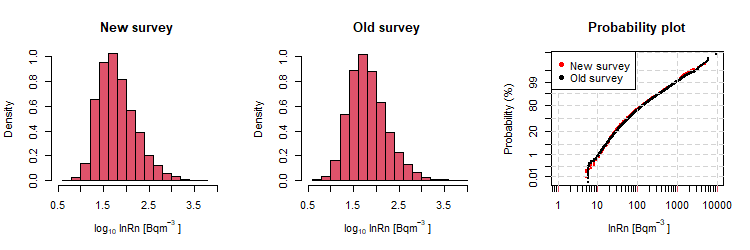
\includegraphics[width=1\linewidth]{Rresults/Figure_7} \end{center}

\hypertarget{figure-8}{%
\subsection{Figure 8}\label{figure-8}}

In-situ vs.~airborne 226Ra concentration in soil (lines represent the
trend lines of the percentiles 2.5th, 50th, 75th and 97.5th obtained in
the simulation; the yellow points are the soil-gas radon samples; and
the black points are the geometric mean of the radon measurements in
each grid).

\begin{Shaded}
\begin{Highlighting}[]
\NormalTok{  p1 \textless{}{-}}\StringTok{ }\KeywordTok{ggplot}\NormalTok{(eU\_Grids1km) }\OperatorTok{+}
\StringTok{  }\KeywordTok{geom\_hline}\NormalTok{(}\DataTypeTok{yintercept =} \KeywordTok{c}\NormalTok{(}\DecValTok{10}\NormalTok{, }\DecValTok{30}\NormalTok{, }\DecValTok{50}\NormalTok{, }\DecValTok{70}\NormalTok{, }\DecValTok{100}\NormalTok{),}
             \DataTypeTok{linetype =} \StringTok{"dashed"}\NormalTok{, }\DataTypeTok{color =} \StringTok{"darkgrey"}\NormalTok{, }\DataTypeTok{size =} \FloatTok{0.5}\NormalTok{) }\OperatorTok{+}
\StringTok{  }\KeywordTok{geom\_point}\NormalTok{(}\KeywordTok{aes}\NormalTok{(}\DataTypeTok{x =}\NormalTok{ AM\_Ra226, }\DataTypeTok{y =}\NormalTok{ Rn\_P025, }\DataTypeTok{colour =} \StringTok{"purple"}\NormalTok{),}
             \DataTypeTok{size =} \FloatTok{0.7}\NormalTok{,}
             \DataTypeTok{alpha =} \FloatTok{0.1}\NormalTok{) }\OperatorTok{+}
\StringTok{  }\KeywordTok{geom\_point}\NormalTok{(}\KeywordTok{aes}\NormalTok{(}\DataTypeTok{x =}\NormalTok{ AM\_Ra226, }\DataTypeTok{y =}\NormalTok{ Rn\_P50, }\DataTypeTok{colour =} \StringTok{"green"}\NormalTok{),}
             \DataTypeTok{size =} \FloatTok{0.7}\NormalTok{,}
             \DataTypeTok{alpha =} \FloatTok{0.1}\NormalTok{) }\OperatorTok{+}
\StringTok{  }\KeywordTok{geom\_point}\NormalTok{(}\KeywordTok{aes}\NormalTok{(}\DataTypeTok{x =}\NormalTok{ AM\_Ra226, }\DataTypeTok{y =}\NormalTok{ Rn\_P75, }\DataTypeTok{colour =} \StringTok{"blue"}\NormalTok{),}
             \DataTypeTok{size =} \FloatTok{0.7}\NormalTok{,}
             \DataTypeTok{alpha =} \FloatTok{0.1}\NormalTok{) }\OperatorTok{+}
\StringTok{  }\KeywordTok{geom\_point}\NormalTok{(}\KeywordTok{aes}\NormalTok{(}\DataTypeTok{x =}\NormalTok{ AM\_Ra226, }\DataTypeTok{y =}\NormalTok{ Rn\_P975, }\DataTypeTok{colour =} \StringTok{"red"}\NormalTok{),}
             \DataTypeTok{size =} \FloatTok{0.7}\NormalTok{,}
             \DataTypeTok{alpha =} \FloatTok{0.1}\NormalTok{) }\OperatorTok{+}
\StringTok{  }\KeywordTok{scale\_colour\_identity}\NormalTok{(}\DataTypeTok{name =} \StringTok{"Percentiles"}\NormalTok{,}
                       \DataTypeTok{breaks =} \KeywordTok{c}\NormalTok{(}\StringTok{"purple"}\NormalTok{, }\StringTok{"green"}\NormalTok{, }\StringTok{"blue"}\NormalTok{, }\StringTok{"red"}\NormalTok{),}
                       \DataTypeTok{labels =} \KeywordTok{c}\NormalTok{(}\StringTok{"2.5th"}\NormalTok{, }\StringTok{"50th"}\NormalTok{, }\StringTok{"75th"}\NormalTok{, }\StringTok{"97.5th"}\NormalTok{),}
                       \DataTypeTok{guide =} \StringTok{"legend"}\NormalTok{) }\OperatorTok{+}
\StringTok{  }\KeywordTok{guides}\NormalTok{(}\DataTypeTok{colour =} \KeywordTok{guide\_legend}\NormalTok{(}\DataTypeTok{override.aes =} \KeywordTok{list}\NormalTok{(}\DataTypeTok{size =} \DecValTok{2}\NormalTok{, }\DataTypeTok{alpha =} \DecValTok{1}\NormalTok{))) }\OperatorTok{+}
\StringTok{  }\KeywordTok{geom\_point}\NormalTok{(}\DataTypeTok{data =}\NormalTok{ Soil\_Rn, }\KeywordTok{aes}\NormalTok{(}\DataTypeTok{x =}\NormalTok{ AM\_Ra226, }\DataTypeTok{y =}\NormalTok{ SoilRn),}
             \DataTypeTok{size =} \FloatTok{0.8}\NormalTok{,}
             \DataTypeTok{colour =} \StringTok{"black"}\NormalTok{) }\OperatorTok{+}
\StringTok{  }\KeywordTok{geom\_point}\NormalTok{(}\DataTypeTok{data =}\NormalTok{ SG\_Sum, }\KeywordTok{aes}\NormalTok{(}\DataTypeTok{x =}\NormalTok{ Ra\_AM, }\DataTypeTok{y =}\NormalTok{ Rn\_GM),}
             \DataTypeTok{colour =} \StringTok{"black"}\NormalTok{,}
             \DataTypeTok{shape =} \DecValTok{18}\NormalTok{,}
             \DataTypeTok{size =} \DecValTok{5}\NormalTok{) }\OperatorTok{+}\StringTok{ }
\StringTok{  }\KeywordTok{xlim}\NormalTok{(}\DecValTok{0}\NormalTok{, }\DecValTok{45}\NormalTok{) }\OperatorTok{+}
\StringTok{  }\KeywordTok{ggtitle}\NormalTok{(}
    \StringTok{"In{-}situ Rn{-}222 soil{-}gas vs. airborne Ra{-}226 (Grids 1km x 1km)"}
\NormalTok{  ) }\OperatorTok{+}\StringTok{ }
\StringTok{  }\KeywordTok{xlab}\NormalTok{(}\KeywordTok{expression}\NormalTok{(}\StringTok{"Mean "}\OperatorTok{*}\StringTok{""}\OperatorTok{\^{}}\DecValTok{226}\OperatorTok{*}\NormalTok{Ra }\OperatorTok{*}\StringTok{ " [ "} \OperatorTok{*}\StringTok{ "Bq "}\OperatorTok{*}\StringTok{ }\NormalTok{kg}\OperatorTok{\^{}{-}}\DecValTok{1} \OperatorTok{*}\StringTok{ " ]"}\NormalTok{)) }\OperatorTok{+}\StringTok{ }
\StringTok{  }\KeywordTok{ylab}\NormalTok{(}\KeywordTok{expression}\NormalTok{(}\StringTok{""}\OperatorTok{\^{}}\DecValTok{222}\OperatorTok{*}\NormalTok{Rn }\OperatorTok{*}\StringTok{ " [ "} \OperatorTok{*}\StringTok{ "kBq "}\OperatorTok{*}\StringTok{ }\NormalTok{m}\OperatorTok{\^{}{-}}\DecValTok{3} \OperatorTok{*}\StringTok{ " ]"}\NormalTok{)) }\OperatorTok{+}
\StringTok{  }\KeywordTok{scale\_y\_log10}\NormalTok{(}\DataTypeTok{breaks =}\NormalTok{ breaks,}
                \DataTypeTok{minor\_breaks =}\NormalTok{ minor\_breaks,}
                \DataTypeTok{limits =} \KeywordTok{c}\NormalTok{(}\DecValTok{1}\NormalTok{, }\DecValTok{1000}\NormalTok{)) }\OperatorTok{+}
\StringTok{  }\KeywordTok{theme\_bw}\NormalTok{()}

  \KeywordTok{ggsave}\NormalTok{(p1,}
         \DataTypeTok{file =} \StringTok{"Rresults/Figure\_8.png"}\NormalTok{,}
         \DataTypeTok{width =} \DecValTok{20}\NormalTok{,}
         \DataTypeTok{height =} \DecValTok{14}\NormalTok{,}
         \DataTypeTok{units =} \StringTok{"cm"}\NormalTok{ )}
\end{Highlighting}
\end{Shaded}

\begin{center}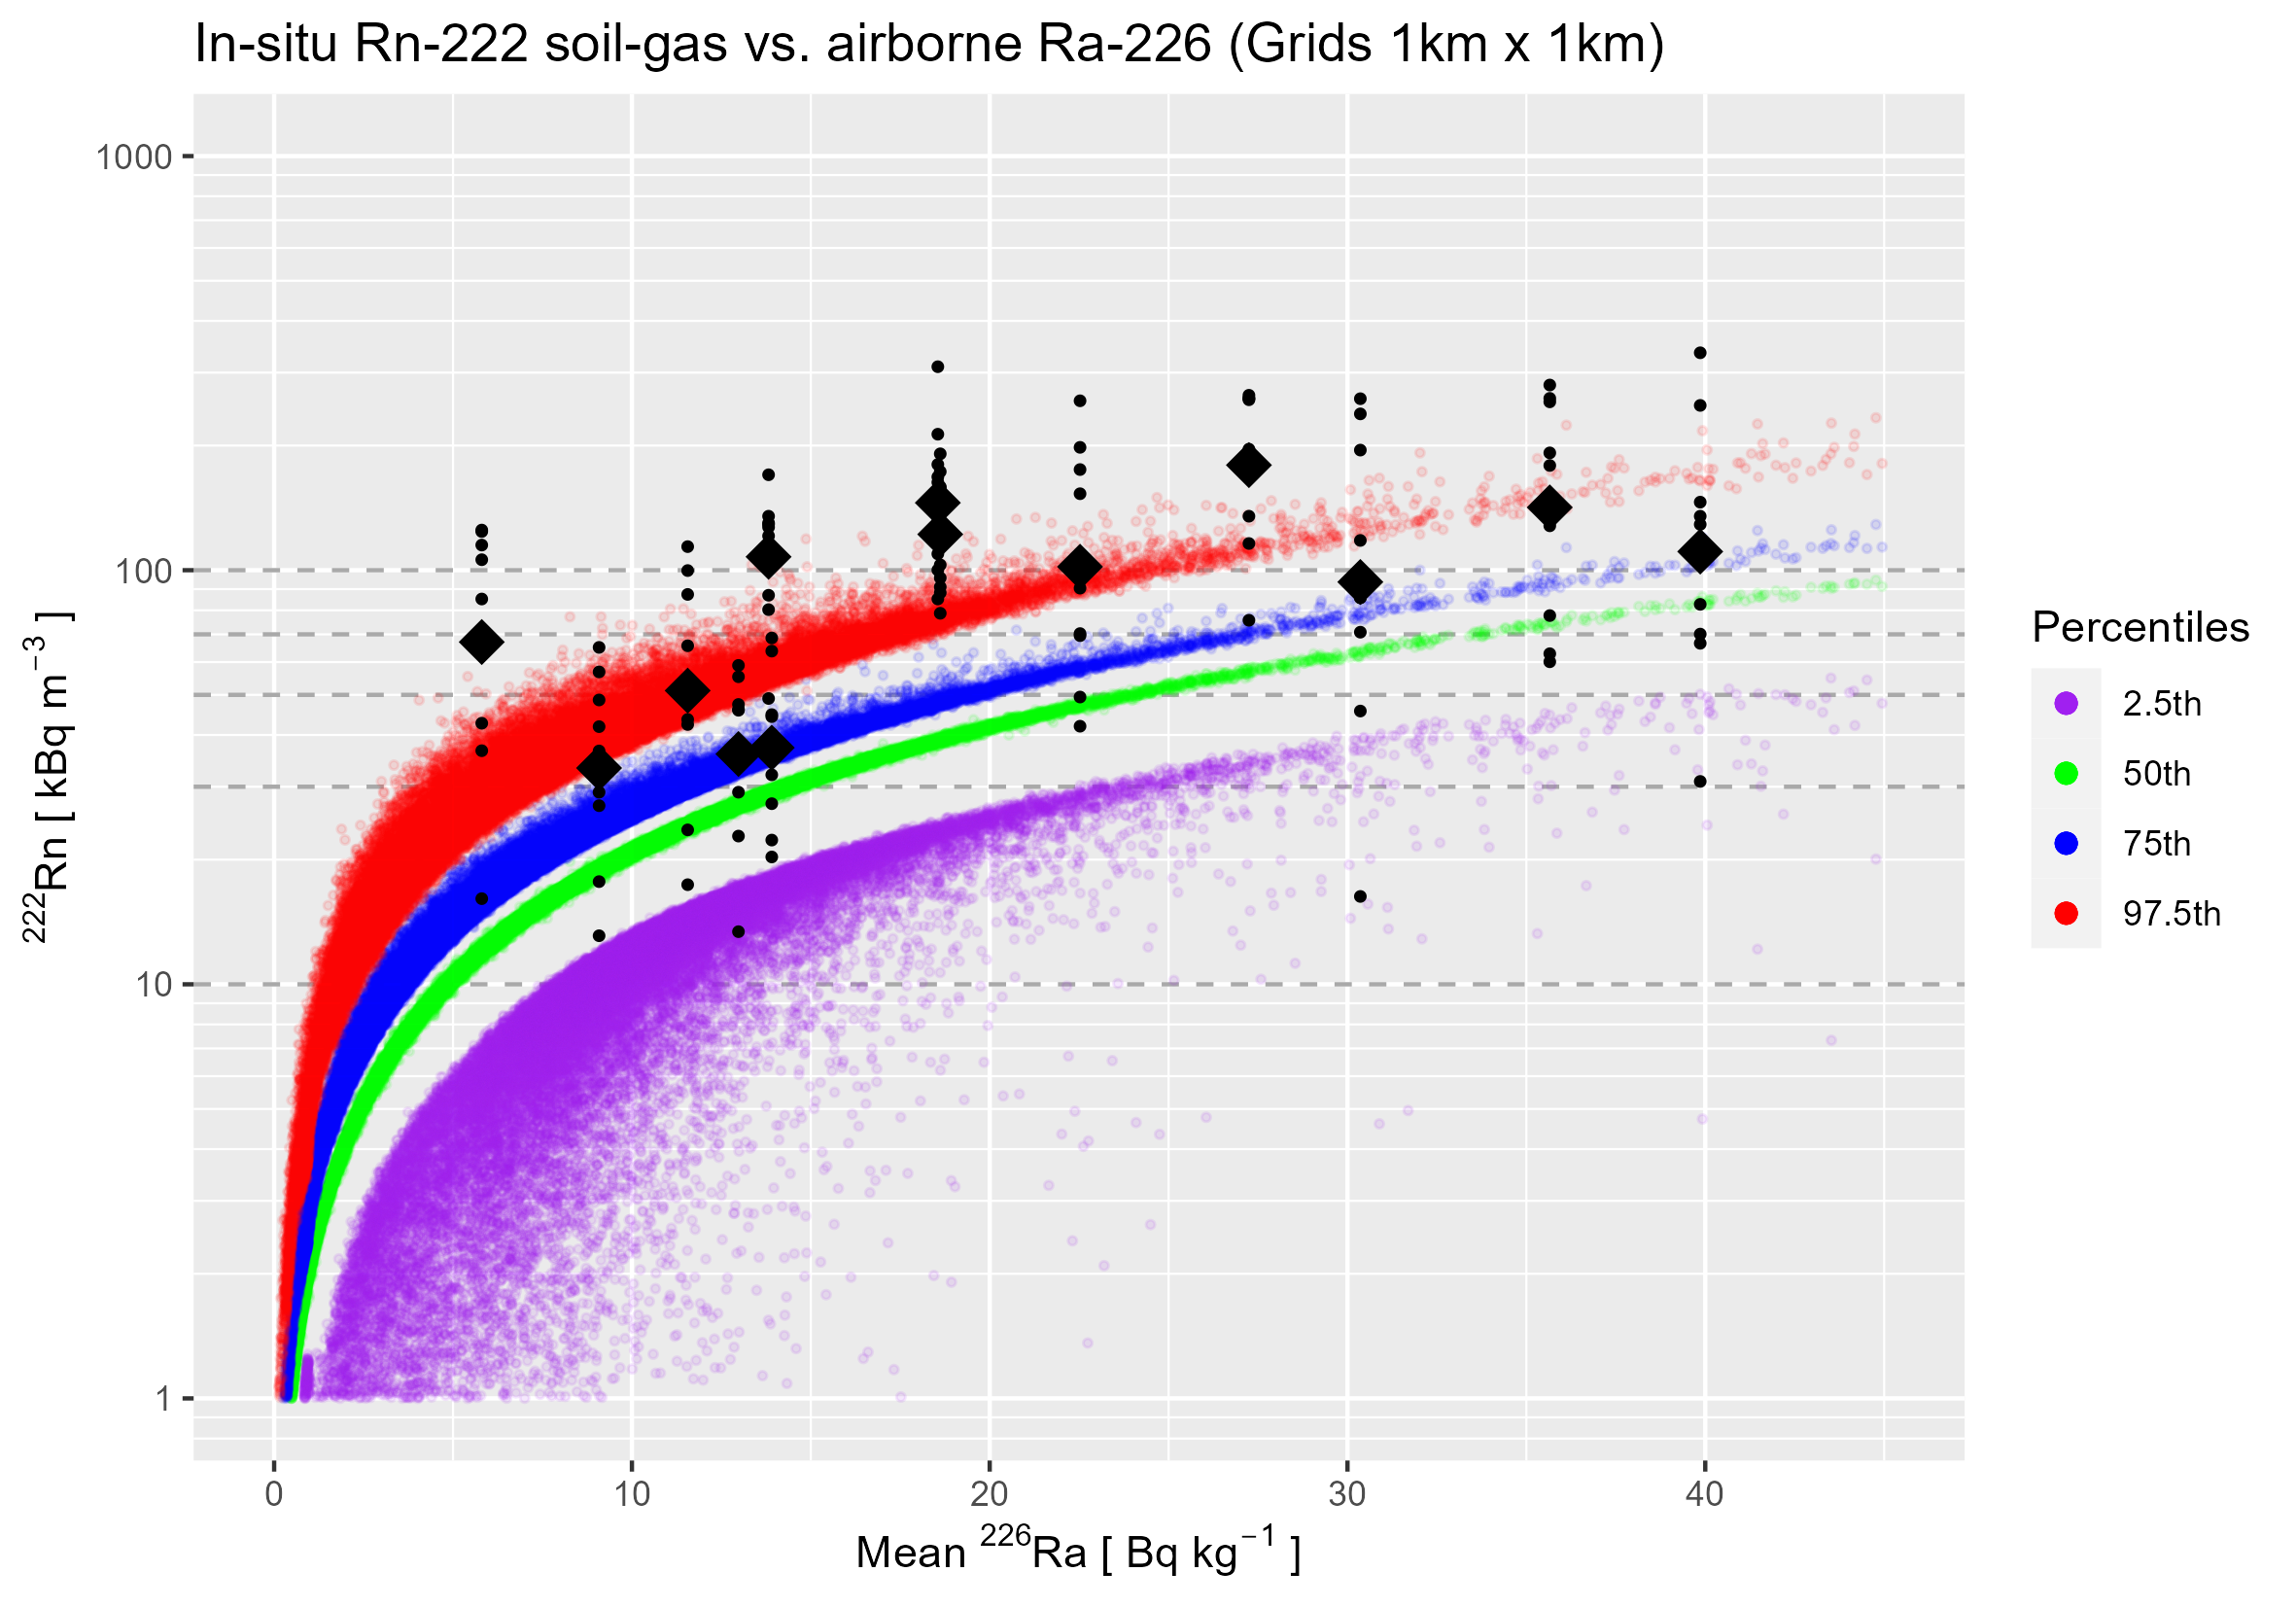
\includegraphics[width=0.5\linewidth]{Rresults/Figure_8} \end{center}

\hypertarget{figure-9}{%
\subsection{Figure 9}\label{figure-9}}

Boxplot of indoor radon measurements (InRn) in each Radon Potential
class (L: Low; ML: Moderate-Low; MH: Moderate-High; and H: High). Boxes
widths are proportional to the square-roots of the number of
observations in each group

\begin{Shaded}
\begin{Highlighting}[]
\NormalTok{  p1 \textless{}{-}}\StringTok{ }\KeywordTok{ggplot}\NormalTok{(InRn\_RP, }\KeywordTok{aes}\NormalTok{(}\DataTypeTok{x =}\NormalTok{ RP\_class, }\DataTypeTok{y =} \KeywordTok{log10}\NormalTok{(InRn))) }\OperatorTok{+}\StringTok{ }
\StringTok{    }\KeywordTok{geom\_boxplot}\NormalTok{(}\DataTypeTok{notch =} \OtherTok{TRUE}\NormalTok{, }\DataTypeTok{fill =} \StringTok{"red"}\NormalTok{) }\OperatorTok{+}
\StringTok{    }\KeywordTok{ylab}\NormalTok{(}\StringTok{"log10(InRn)"}\NormalTok{) }\OperatorTok{+}
\StringTok{    }\KeywordTok{xlab}\NormalTok{(}\StringTok{"GRP"}\NormalTok{)}

  \KeywordTok{ggsave}\NormalTok{(p1,}
         \DataTypeTok{file =} \StringTok{"Rresults/Figure\_9.png"}\NormalTok{,}
         \DataTypeTok{width =} \DecValTok{7}\NormalTok{,}
         \DataTypeTok{height =} \DecValTok{7}\NormalTok{,}
         \DataTypeTok{units =} \StringTok{"cm"}\NormalTok{ )}
\end{Highlighting}
\end{Shaded}

\begin{center}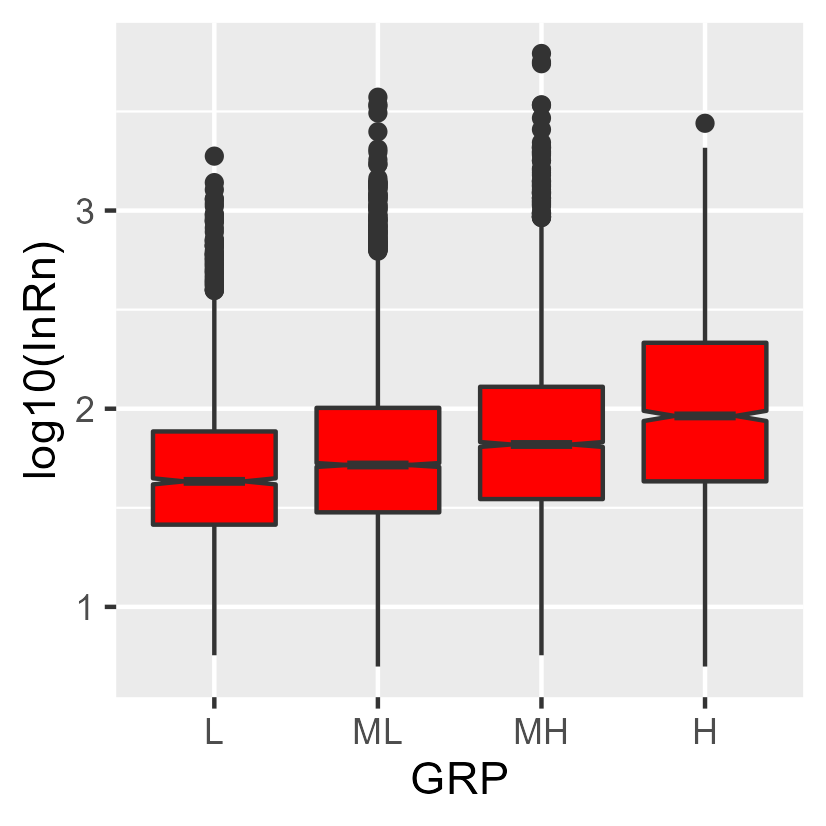
\includegraphics[width=0.5\linewidth]{Rresults/Figure_9} \end{center}

\end{document}
